\PassOptionsToPackage{unicode=true}{hyperref} % options for packages loaded elsewhere
\PassOptionsToPackage{hyphens}{url}
%
\documentclass[]{book}
\usepackage{lmodern}
\usepackage{amssymb,amsmath}
\usepackage{ifxetex,ifluatex}
\usepackage{fixltx2e} % provides \textsubscript
\ifnum 0\ifxetex 1\fi\ifluatex 1\fi=0 % if pdftex
  \usepackage[T1]{fontenc}
  \usepackage[utf8]{inputenc}
  \usepackage{textcomp} % provides euro and other symbols
\else % if luatex or xelatex
  \usepackage{unicode-math}
  \defaultfontfeatures{Ligatures=TeX,Scale=MatchLowercase}
\fi
% use upquote if available, for straight quotes in verbatim environments
\IfFileExists{upquote.sty}{\usepackage{upquote}}{}
% use microtype if available
\IfFileExists{microtype.sty}{%
\usepackage[]{microtype}
\UseMicrotypeSet[protrusion]{basicmath} % disable protrusion for tt fonts
}{}
\IfFileExists{parskip.sty}{%
\usepackage{parskip}
}{% else
\setlength{\parindent}{0pt}
\setlength{\parskip}{6pt plus 2pt minus 1pt}
}
\usepackage{hyperref}
\hypersetup{
            pdftitle={MA 5124 Financial Time Series Analysis \& Forecasting},
            pdfauthor={Dr.~Priyanga D. Talagala},
            pdfborder={0 0 0},
            breaklinks=true}
\urlstyle{same}  % don't use monospace font for urls
\usepackage{color}
\usepackage{fancyvrb}
\newcommand{\VerbBar}{|}
\newcommand{\VERB}{\Verb[commandchars=\\\{\}]}
\DefineVerbatimEnvironment{Highlighting}{Verbatim}{commandchars=\\\{\}}
% Add ',fontsize=\small' for more characters per line
\usepackage{framed}
\definecolor{shadecolor}{RGB}{248,248,248}
\newenvironment{Shaded}{\begin{snugshade}}{\end{snugshade}}
\newcommand{\AlertTok}[1]{\textcolor[rgb]{0.94,0.16,0.16}{#1}}
\newcommand{\AnnotationTok}[1]{\textcolor[rgb]{0.56,0.35,0.01}{\textbf{\textit{#1}}}}
\newcommand{\AttributeTok}[1]{\textcolor[rgb]{0.77,0.63,0.00}{#1}}
\newcommand{\BaseNTok}[1]{\textcolor[rgb]{0.00,0.00,0.81}{#1}}
\newcommand{\BuiltInTok}[1]{#1}
\newcommand{\CharTok}[1]{\textcolor[rgb]{0.31,0.60,0.02}{#1}}
\newcommand{\CommentTok}[1]{\textcolor[rgb]{0.56,0.35,0.01}{\textit{#1}}}
\newcommand{\CommentVarTok}[1]{\textcolor[rgb]{0.56,0.35,0.01}{\textbf{\textit{#1}}}}
\newcommand{\ConstantTok}[1]{\textcolor[rgb]{0.00,0.00,0.00}{#1}}
\newcommand{\ControlFlowTok}[1]{\textcolor[rgb]{0.13,0.29,0.53}{\textbf{#1}}}
\newcommand{\DataTypeTok}[1]{\textcolor[rgb]{0.13,0.29,0.53}{#1}}
\newcommand{\DecValTok}[1]{\textcolor[rgb]{0.00,0.00,0.81}{#1}}
\newcommand{\DocumentationTok}[1]{\textcolor[rgb]{0.56,0.35,0.01}{\textbf{\textit{#1}}}}
\newcommand{\ErrorTok}[1]{\textcolor[rgb]{0.64,0.00,0.00}{\textbf{#1}}}
\newcommand{\ExtensionTok}[1]{#1}
\newcommand{\FloatTok}[1]{\textcolor[rgb]{0.00,0.00,0.81}{#1}}
\newcommand{\FunctionTok}[1]{\textcolor[rgb]{0.00,0.00,0.00}{#1}}
\newcommand{\ImportTok}[1]{#1}
\newcommand{\InformationTok}[1]{\textcolor[rgb]{0.56,0.35,0.01}{\textbf{\textit{#1}}}}
\newcommand{\KeywordTok}[1]{\textcolor[rgb]{0.13,0.29,0.53}{\textbf{#1}}}
\newcommand{\NormalTok}[1]{#1}
\newcommand{\OperatorTok}[1]{\textcolor[rgb]{0.81,0.36,0.00}{\textbf{#1}}}
\newcommand{\OtherTok}[1]{\textcolor[rgb]{0.56,0.35,0.01}{#1}}
\newcommand{\PreprocessorTok}[1]{\textcolor[rgb]{0.56,0.35,0.01}{\textit{#1}}}
\newcommand{\RegionMarkerTok}[1]{#1}
\newcommand{\SpecialCharTok}[1]{\textcolor[rgb]{0.00,0.00,0.00}{#1}}
\newcommand{\SpecialStringTok}[1]{\textcolor[rgb]{0.31,0.60,0.02}{#1}}
\newcommand{\StringTok}[1]{\textcolor[rgb]{0.31,0.60,0.02}{#1}}
\newcommand{\VariableTok}[1]{\textcolor[rgb]{0.00,0.00,0.00}{#1}}
\newcommand{\VerbatimStringTok}[1]{\textcolor[rgb]{0.31,0.60,0.02}{#1}}
\newcommand{\WarningTok}[1]{\textcolor[rgb]{0.56,0.35,0.01}{\textbf{\textit{#1}}}}
\usepackage{longtable,booktabs}
% Fix footnotes in tables (requires footnote package)
\IfFileExists{footnote.sty}{\usepackage{footnote}\makesavenoteenv{longtable}}{}
\usepackage{graphicx,grffile}
\makeatletter
\def\maxwidth{\ifdim\Gin@nat@width>\linewidth\linewidth\else\Gin@nat@width\fi}
\def\maxheight{\ifdim\Gin@nat@height>\textheight\textheight\else\Gin@nat@height\fi}
\makeatother
% Scale images if necessary, so that they will not overflow the page
% margins by default, and it is still possible to overwrite the defaults
% using explicit options in \includegraphics[width, height, ...]{}
\setkeys{Gin}{width=\maxwidth,height=\maxheight,keepaspectratio}
\setlength{\emergencystretch}{3em}  % prevent overfull lines
\providecommand{\tightlist}{%
  \setlength{\itemsep}{0pt}\setlength{\parskip}{0pt}}
\setcounter{secnumdepth}{5}
% Redefines (sub)paragraphs to behave more like sections
\ifx\paragraph\undefined\else
\let\oldparagraph\paragraph
\renewcommand{\paragraph}[1]{\oldparagraph{#1}\mbox{}}
\fi
\ifx\subparagraph\undefined\else
\let\oldsubparagraph\subparagraph
\renewcommand{\subparagraph}[1]{\oldsubparagraph{#1}\mbox{}}
\fi

% set default figure placement to htbp
\makeatletter
\def\fps@figure{htbp}
\makeatother

\usepackage{booktabs}
\usepackage{amsthm}
\makeatletter
\def\thm@space@setup{%
  \thm@preskip=8pt plus 2pt minus 4pt
  \thm@postskip=\thm@preskip
}
\makeatother
\usepackage{fancyhdr}
\pagestyle{fancy}
\fancyfoot[CO,CE]{Prepared by Dr. Priyanga D. Talagala  (Copyright 2021 Priyanga D. Talagala)}
\fancyfoot[LE,RO]{\thepage}
\usepackage{float}
\usepackage[]{natbib}
\bibliographystyle{apalike}

\title{MA 5124 Financial Time Series Analysis \& Forecasting}
\author{Dr.~Priyanga D. Talagala}
\date{2021-02-26}

\begin{document}
\maketitle

{
\setcounter{tocdepth}{1}
\tableofcontents
}
\hypertarget{course-syllabus}{%
\chapter*{Course Syllabus}\label{course-syllabus}}
\addcontentsline{toc}{chapter}{Course Syllabus}

\pagenumbering{arabic}

\textbf{Module Code:} MA 5124

\textbf{Title:} Financial Time Series Analysis \& Forecasting

\textbf{Credits:} 4

\hypertarget{pre-requiites}{%
\section*{Pre-requiites}\label{pre-requiites}}
\addcontentsline{toc}{section}{Pre-requiites}

None

\hypertarget{learning-objectives}{%
\section*{Learning Objectives}\label{learning-objectives}}
\addcontentsline{toc}{section}{Learning Objectives}

\begin{itemize}
\tightlist
\item
  The purpose of this course is to provide students with introductory tools for the time series analysis of financial time series.
\item
  Analyze of data series based on stochastic and non stochastic models
\end{itemize}

\hypertarget{learning-outcomes}{%
\section*{Learning Outcomes}\label{learning-outcomes}}
\addcontentsline{toc}{section}{Learning Outcomes}

\begin{itemize}
\tightlist
\item
  On successful completion of this course, students will be able to provide more than an introductory treatment of the topics.
\item
  Students are encouraged to pursue further study in this area if they find that the topics covered in this course.
\end{itemize}

\hypertarget{outline-syllabus}{%
\section*{Outline Syllabus}\label{outline-syllabus}}
\addcontentsline{toc}{section}{Outline Syllabus}

\begin{itemize}
\tightlist
\item
  Definition and examples of time series
\item
  back-shift and differencing-operators, - strong and weak stationarity, definition of ACF, PACF.
\item
  Definitions and properties of the \(MA(q), MA(\infty), AR(p), AR(\infty)\)
  and \(ARMA(p,q)\),in particualr their acf's
\item
  causal stationarity of AR
\item
  invertibility of MA models and causal stationarity and invertibility of ARMA; - concept of spectral density function and its applications
\item
  definition and properties of integrated \(ARIMA(p,d,q)\) processes
\item
  definition and properties of random walks with or without drift.
\item
  Model selection following the AIC and BIC
\item
  brief introduction to linear prediction and calculation of forecasting intervals for normal ARMA models
\item
  point and interval forecasts for normal random walks with or without drift.
\item
  Definition and properties of the VAR (vector autoregressive) model, arrange a univariate time series as a multivariate Markov model.
\item
  Nonlinear properties of financial time series
\item
  definition and properties of the well known ARCH, GARCH etc.
\item
  Cointegration in Single Equations, Modeling and Forecasting Financial Time Series.
\end{itemize}

\hypertarget{method-of-assessment}{%
\section*{Method of Assessment}\label{method-of-assessment}}
\addcontentsline{toc}{section}{Method of Assessment}

\begin{itemize}
\tightlist
\item
  Assignment 30\%
\item
  End-semester examination 70\%
\end{itemize}

\hypertarget{lecturer}{%
\section*{Lecturer}\label{lecturer}}
\addcontentsline{toc}{section}{Lecturer}

Dr.~Priyanga D. Talagala

\hypertarget{schedule}{%
\section*{Schedule}\label{schedule}}
\addcontentsline{toc}{section}{Schedule}

Lectures:

\begin{itemize}
\tightlist
\item
  Sunday {[}9.00am -12.00 noon{]}
\end{itemize}

\hypertarget{copyright-notice}{%
\section*{Copyright Notice}\label{copyright-notice}}
\addcontentsline{toc}{section}{Copyright Notice}

My lectures and course materials, including presentations, tests, exams, outlines, and similar materials, are protected by copyright. I am the exclusive owner of copyright in those materials I create. I encourage you to take notes and make copies of course materials for your own educational use. However, you may not, nor may you knowingly allow others to reproduce or distribute lecture notes and course materials publicly without my express written consent.

\hypertarget{intro}{%
\chapter{Intordution to Time Series Forecasting}\label{intro}}

\hypertarget{arima-models}{%
\chapter{ARIMA models}\label{arima-models}}

\pagenumbering{arabic}

\begin{itemize}
\tightlist
\item
  \textbf{AR}: autoregressive (lagged observations as inputs)
\item
  \textbf{I}: integrated (differencing to make series stationary)
\item
  \textbf{MA}: moving average (lagged errors as inputs)
\end{itemize}

An ARIMA model is rarely interpretable in terms of visible data structures like trend and seasonality. But it can capture a huge range of time series patterns.

\hypertarget{stationarity-and-differencing}{%
\section{Stationarity and differencing}\label{stationarity-and-differencing}}

\hypertarget{stationarity}{%
\subsection{Stationarity}\label{stationarity}}

\textbf{Definition}

If \(\{y_t\}\) is a stationary time series, then for all \(s\), the distribution of \((y_t,\dots,y_{t+s})\) does not depend on \(t\).

A \textbf{stationary series} is:

\begin{itemize}
\item
  roughly horizontal
\item
  constant variance
\item
  no patterns predictable in the long-term
\item
  Transformations help to stabilize the variance.
\item
  For ARIMA modelling, we also need to stabilize the mean.
\end{itemize}

\newpage

\textbf{Identifying non-stationary series}

\begin{itemize}
\tightlist
\item
  time plot.
\item
  The ACF of stationary data drops to zero relatively quickly
\item
  The ACF of non-stationary data decreases slowly.
\item
  For non-stationary data, the value of r1 is often large and positive.
\end{itemize}

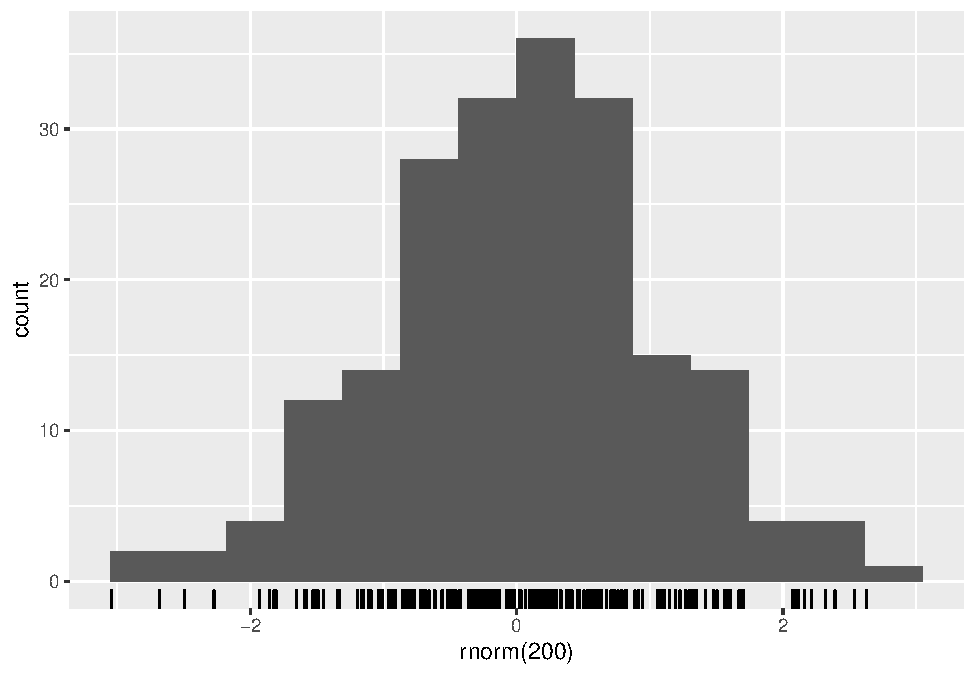
\includegraphics{bookdown-demo_files/figure-latex/unnamed-chunk-1-1.pdf}

\begin{itemize}
\tightlist
\item
  A time series, \(\{Y_t, t=0, \pm1,\dots\}\) is said to be \textbf{strict stationary}, if \((Y_1, \dots, Y_n)\) and \((Y_{1+h}, \dots, Y_{n+h})\) have the same joint distribution for all integers \(h\) and \(n>0.\)
\end{itemize}

\hypertarget{weak-stationarity}{%
\subsubsection{Weak Stationarity}\label{weak-stationarity}}

\textbf{Definition: Covariance function} (in \citep{brockwell2016introduction}, p.~15; the notations have been changed for consistency within this note)

Let \(\{Y_t\}\) be a time series with \(E(Y_t^2)<\infty.\) The \textbf{mean function} of \(\{Y_t\}\) is

\[\mu_Y(t)= E(Y_t)\]

The \textbf{covariance function} of \(\{Y_t\}\) is

\[\gamma_Y(r,s)=Cov(Y_r, Y_s)=E[(Y_r-\mu_Y(r))(Y_s-\mu_Y(s))]\]

for all integers \(r\) and \(s\).

\textbf{Definition: Weakly stationary} (in \citep{brockwell2016introduction}, p.~15; the notations have been changed for consistency within this note)

\(\{Y_t\}\) is \textbf{weakly stationary} if

\begin{enumerate}
\def\labelenumi{\arabic{enumi}.}
\tightlist
\item
  \(\mu_Y(t)\) is independent of \(t\),
\end{enumerate}

and

\begin{enumerate}
\def\labelenumi{\arabic{enumi}.}
\setcounter{enumi}{1}
\tightlist
\item
  \(\gamma_Y(t+h,t)\) is independent of \(t\) for each \(h\).
\end{enumerate}

\begin{itemize}
\tightlist
\item
  Unless specifically indicate otherwise, whenever we use the term \emph{stationary} we shall mean \emph{weakly stationary}.
\end{itemize}

\hypertarget{differencing}{%
\subsection{Differencing}\label{differencing}}

\begin{itemize}
\tightlist
\item
  Differencing helps to \textbf{stabilize the mean}.
\item
  The differenced series is the \emph{change} between each observation in the original series: \(y'_t = y_t - y_{t-1}\).
\item
  The differenced series will have only \(T-1\) values since it is not possible to calculate a difference \(y_1'\) for the first observation.
\end{itemize}

\hypertarget{second-order-differencing}{%
\subsubsection{Second-order differencing}\label{second-order-differencing}}

Occasionally the differenced data will not appear stationary and it may be necessary to difference the data a second time:

\[y''_{t} = y'_{t} - y'_{t - 1}\]
\[= (y_t - y_{t-1}) - (y_{t-1}-y_{t-2})\]
\[= y_t - 2y_{t-1} +y_{t-2}.\]

\begin{itemize}
\tightlist
\item
  \(y_t''\) will have \(T-2\) values.
\item
  In practice, it is almost never necessary to go beyond second-order differences.
\end{itemize}

\hypertarget{seasonal-differencing}{%
\subsubsection{Seasonal differencing}\label{seasonal-differencing}}

A seasonal difference is the difference between an observation and the corresponding observation from the previous year.

\[y'_t = y_t - y_{t-m}\]

where \(m=\) number of seasons.

\begin{itemize}
\tightlist
\item
  For monthly data \(m=12\).
\item
  For quarterly data \(m=4\).
\end{itemize}

\newpage

\textbf{Example : Electricity production}

\begin{Shaded}
\begin{Highlighting}[]
\NormalTok{usmelec }\OperatorTok\StringTok{ }\KeywordTok{autoplot}\NormalTok{(Generation)}
\end{Highlighting}
\end{Shaded}

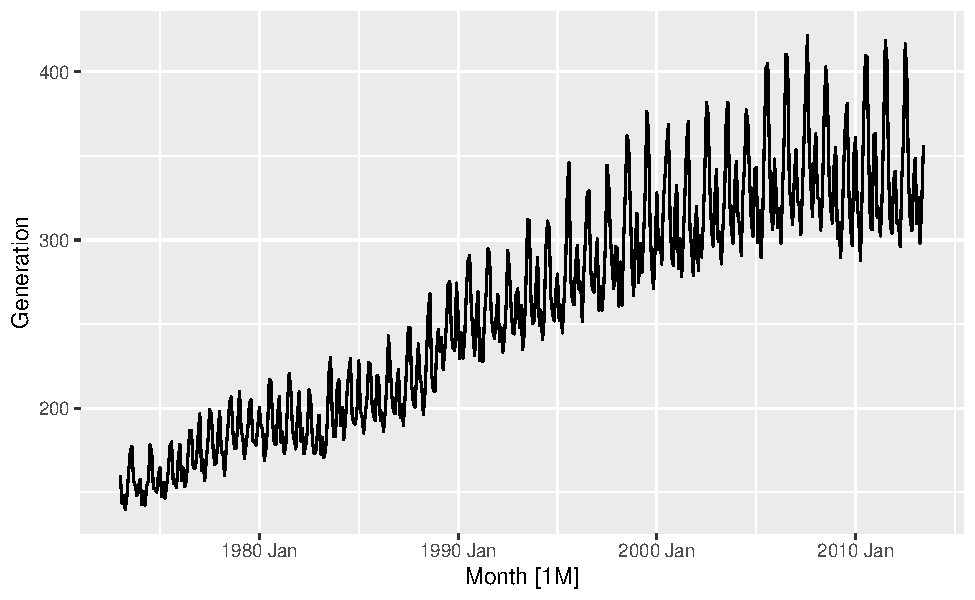
\includegraphics{bookdown-demo_files/figure-latex/unnamed-chunk-3-1.pdf}

\begin{Shaded}
\begin{Highlighting}[]
\NormalTok{usmelec }\OperatorTok\StringTok{ }\KeywordTok{autoplot}\NormalTok{(}\KeywordTok{log}\NormalTok{(Generation))}
\end{Highlighting}
\end{Shaded}

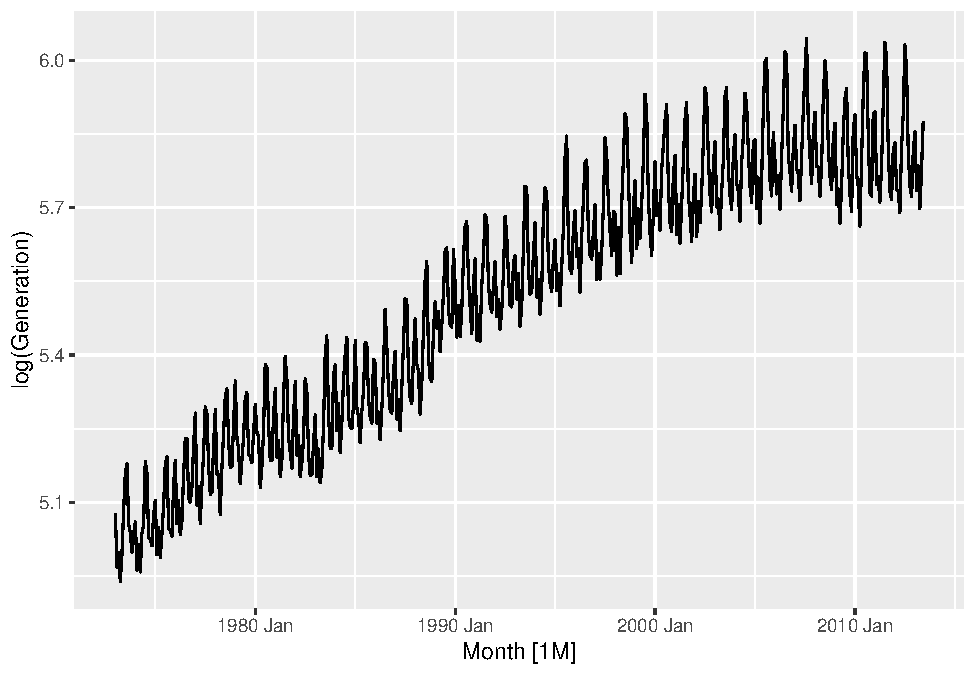
\includegraphics{bookdown-demo_files/figure-latex/unnamed-chunk-4-1.pdf}

\begin{Shaded}
\begin{Highlighting}[]
\NormalTok{usmelec }\OperatorTok\StringTok{ }\KeywordTok{autoplot}\NormalTok{(}\KeywordTok{log}\NormalTok{(Generation) }\OperatorTok\StringTok{ }\KeywordTok{difference}\NormalTok{(}\DecValTok{12}\NormalTok{)) }
\end{Highlighting}
\end{Shaded}

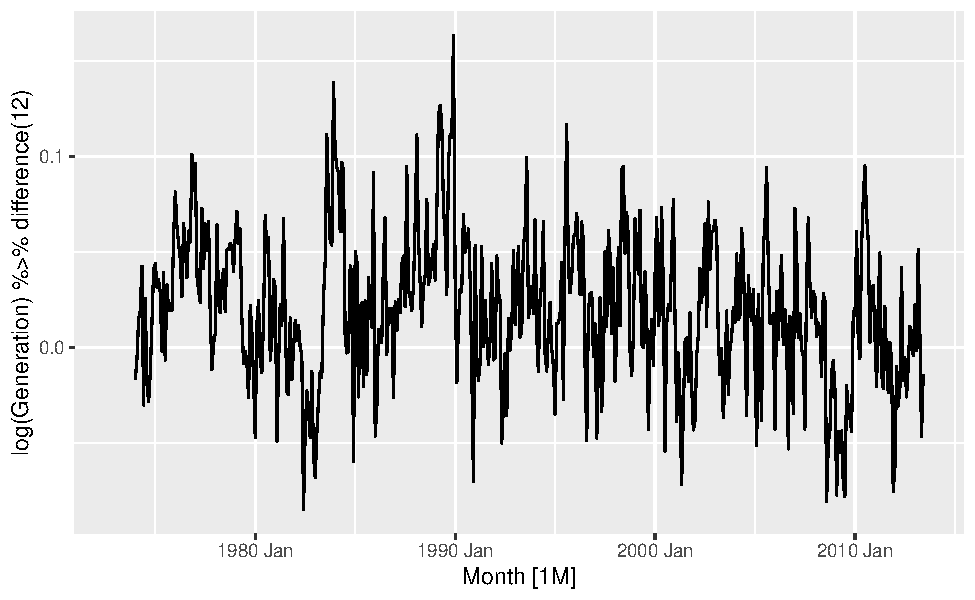
\includegraphics{bookdown-demo_files/figure-latex/unnamed-chunk-5-1.pdf}

\begin{Shaded}
\begin{Highlighting}[]
\NormalTok{ usmelec }\OperatorTok\StringTok{ }\KeywordTok{autoplot}\NormalTok{(}\KeywordTok{log}\NormalTok{(Generation) }\OperatorTok\StringTok{ }\KeywordTok{difference}\NormalTok{(}\DecValTok{12}\NormalTok{) }\OperatorTok\StringTok{ }\KeywordTok{difference}\NormalTok{())}
\end{Highlighting}
\end{Shaded}

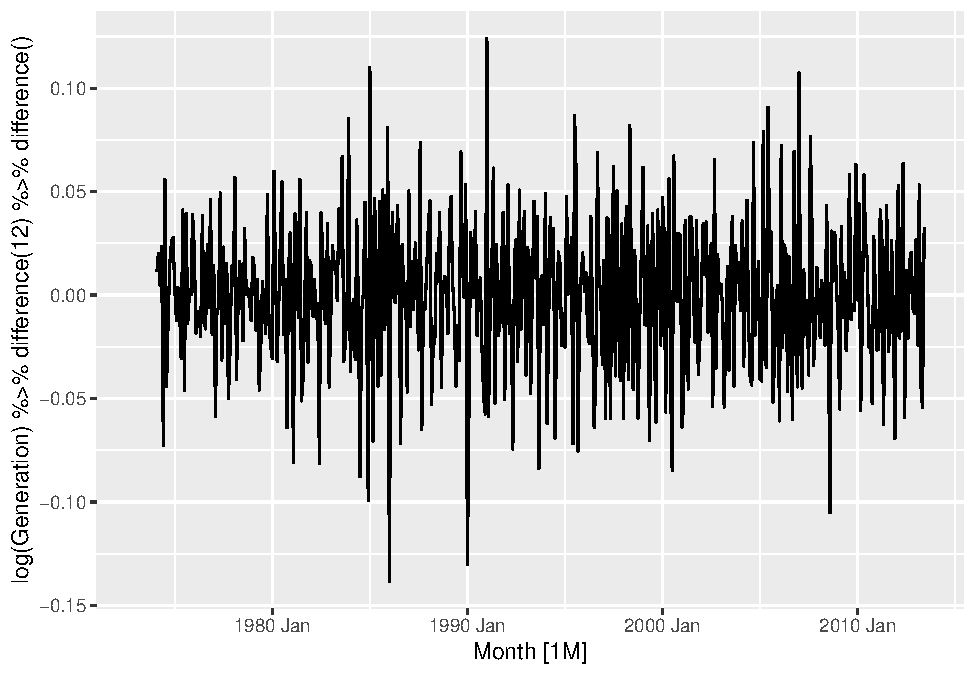
\includegraphics{bookdown-demo_files/figure-latex/unnamed-chunk-6-1.pdf}

\begin{itemize}
\tightlist
\item
  Seasonally differenced series is closer to being stationary.
\item
  Remaining non-stationarity can be removed with further first difference.
\end{itemize}

If \(y'_t = y_t - y_{t-12}\) denotes seasonally differenced series, then twice-differenced series is

\[y^*_t = y'_t - y'_{t-1}\]
\[= (y_t - y_{t-12}) - (y_{t-1} - y_{t-13})\]
\[= y_t - y_{t-1} - y_{t-12} + y_{t-13}.\]

When both seasonal and first differences are applied \(\dots\)

\begin{itemize}
\tightlist
\item
  it makes no difference which is done first---the result will be the same.
\item
  If seasonality is strong, we recommend that seasonal differencing be done first because sometimes the resulting series will be stationary and there will be no need for further first difference.
\end{itemize}

It is important that if differencing is used, the differences are interpretable.

\hypertarget{interpretation-of-differencing}{%
\subsubsection{Interpretation of differencing}\label{interpretation-of-differencing}}

\begin{itemize}
\tightlist
\item
  first differences are the change between one observation and the next;
\item
  seasonal differences are the change between one year to the next.
\end{itemize}

But taking lag 3 differences for yearly data, for example, results in a model which cannot be sensibly interpreted.

\hypertarget{backshift-notation}{%
\subsection{Backshift notation}\label{backshift-notation}}

A very useful notational device is the backward shift operator, \(B\), which is used as follows:
\[B y_{t} = y_{t - 1}\]

In other words,

\begin{itemize}
\item
  \(B\), operating on \(y_{t}\), has the effect of \textbf{shifting the data back one period}.
\item
  Two applications of \(B\) to \(y_{t}\) \textbf{shifts the data back two periods}:
  \[B(By_{t}) = B^{2}y_{t} = y_{t-2}\]
\item
  For monthly data, if we wish to shift attention to ``the same month last year'', then \(B^{12}\) is used, and the notation is \[B^{12}y_{t} = y_{t-12}\].
\item
  The backward shift operator is convenient for describing the process of \emph{differencing}.
\item
  A first difference can be written as
  \[y^{\prime}_{t}= y_{t} - y_{t-1}= y_t - By_{t} = (1 - B)y_{t}\]
\item
  Note that a first difference is represented by \((1 - B)\).
\item
  Similarly, if second-order differences (i.e., first differences of first differences) have to be computed, then:
  \[y''_{t} = y_{t} - 2y_{t - 1} + y_{t - 2} = (1 - B)^{2} y_{t}\]
\item
  Second-order difference is denoted \((1- B)^{2}\).
\item
  \emph{Second-order difference} is not the same as a \emph{second difference}, which would be denoted \(1- B^{2}\);
\item
  In general, a \(d\)th-order difference can be written as
\end{itemize}

\[(1 - B)^{d} y_{t}\]
* A seasonal difference followed by a first difference can be written as

\[(1-B)(1-B^m)y_t\]
- The ``backshift'' notation is convenient because the terms can be multiplied together to see the combined effect.

\[(1-B)(1-B^m)y_t = (1 - B - B^m + B^{m+1})y_t\]
\[= y_t-y_{t-1}-y_{t-m}+y_{t-m-1}.\]
- For monthly data, \(m=12\) and we obtain the same result as earlier.

\hypertarget{non-seasonal-arima-models}{%
\section{Non-seasonal ARIMA models}\label{non-seasonal-arima-models}}

\hypertarget{autoregressive-models}{%
\subsection{Autoregressive models}\label{autoregressive-models}}

\textbf{Autoregressive (AR) models:}
\[y_{t} = c + \phi_{1}y_{t - 1} + \phi_{2}y_{t - 2} + \cdots + \phi_{p}y_{t - p} + \varepsilon_{t},\]
where \(\varepsilon_t\) is white noise. This is a multiple regression with \textbf{lagged values} of \(y_t\) as predictors.

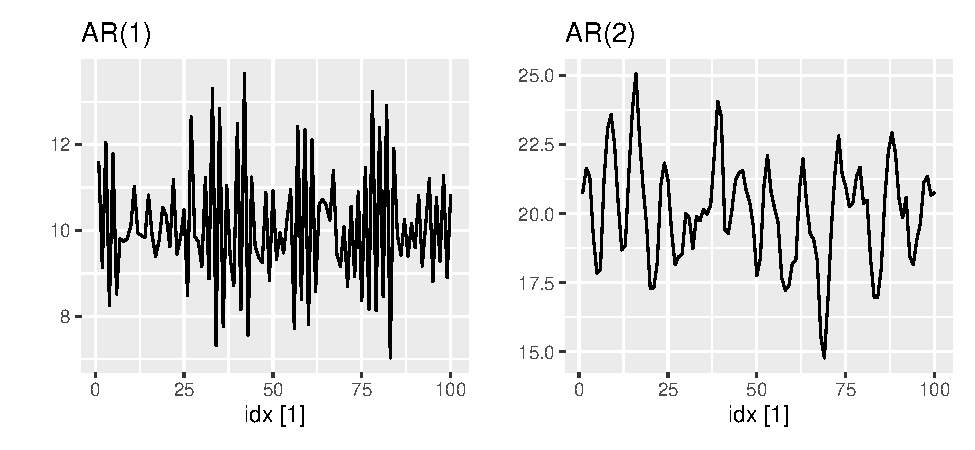
\includegraphics{bookdown-demo_files/figure-latex/arp-1.pdf}

\hypertarget{ar1-model}{%
\subsubsection{AR(1) model}\label{ar1-model}}

\[y_{t} = 18 -0.8 y_{t - 1} + \varepsilon_{t}\]
\[\varepsilon_t\sim N(0,1),\quad T=100.\]

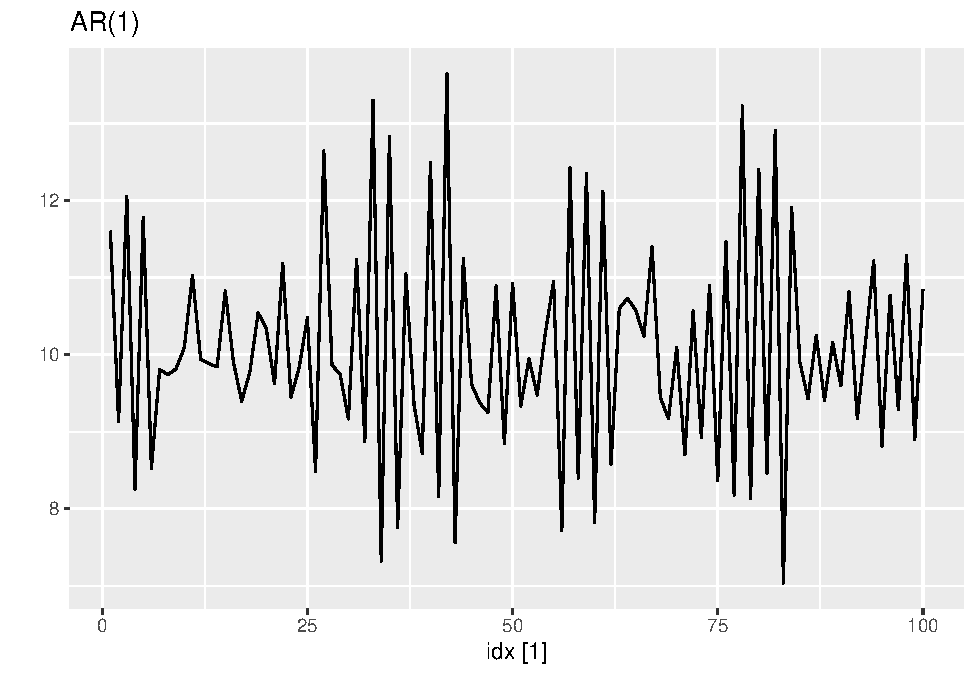
\includegraphics{bookdown-demo_files/figure-latex/unnamed-chunk-7-1.pdf}

\[y_{t} = c + \phi_1 y_{t - 1} + \varepsilon_{t}\]

\begin{itemize}
\tightlist
\item
  When \(\phi_1=0\), \(y_t\) is \textbf{equivalent to WN}
\item
  When \(\phi_1=1\) and \(c=0\), \(y_t\) is \textbf{equivalent to a RW}
\item
  When \(\phi_1=1\) and \(c\ne0\), \(y_t\) is \textbf{equivalent to a RW with drift}
\item
  When \(\phi_1<0\), \(y_t\) tends to \textbf{oscillate between positive and negative values}.
\end{itemize}

\hypertarget{ar2-model}{%
\subsubsection{AR(2) model}\label{ar2-model}}

\[y_t = 8 + 1.3y_{t-1} - 0.7 y_{t-2} + \varepsilon_t\]
\[\varepsilon_t\sim N(0,1), \qquad T=100.\]

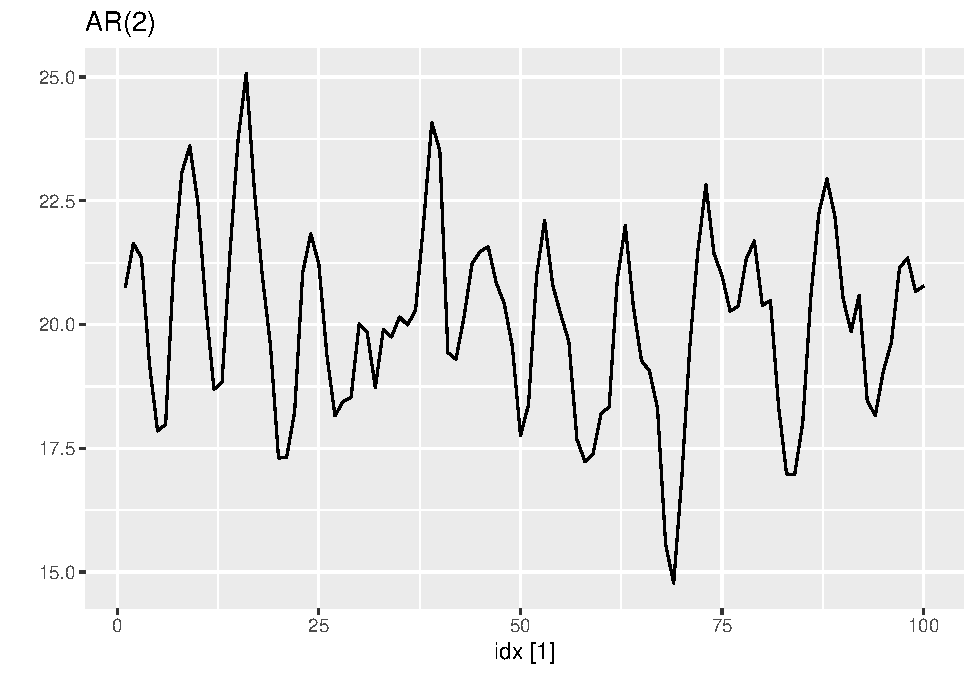
\includegraphics{bookdown-demo_files/figure-latex/unnamed-chunk-8-1.pdf}

\hypertarget{stationarity-conditions}{%
\subsubsection{Stationarity conditions}\label{stationarity-conditions}}

\begin{itemize}
\tightlist
\item
  We normally restrict autoregressive models to stationary data, and then some constraints on the values of the parameters are required.
\end{itemize}

\textbf{General condition for stationarity}

Complex roots of \(1-\phi_1 z - \phi_2 z^2 - \dots - \phi_pz^p\) lie outside the unit circle on the complex plane.

\begin{itemize}
\tightlist
\item
  For \(p=1\): \(-1<\phi_1<1\).
\item
  For \(p=2\):\newline \(-1<\phi_2<1\qquad \phi_2+\phi_1 < 1 \qquad \phi_2 -\phi_1 < 1\).
\item
  More complicated conditions hold for \(p\ge3\).
\item
  Estimation software takes care of this.
\end{itemize}

\hypertarget{moving-average-ma-models}{%
\subsection{Moving Average (MA) models}\label{moving-average-ma-models}}

\textbf{Moving Average (MA) models:}
\[y_{t} = c + \varepsilon_t + \theta_{1}\varepsilon_{t - 1} + \theta_{2}\varepsilon_{t - 2} + \cdots + \theta_{q}\varepsilon_{t - q},\]
where \(\varepsilon_t\) is white noise.
This is a multiple regression with \textbf{past errors} as predictors.

\begin{itemize}
\tightlist
\item
  Don't confuse this with moving average smoothing!
\end{itemize}

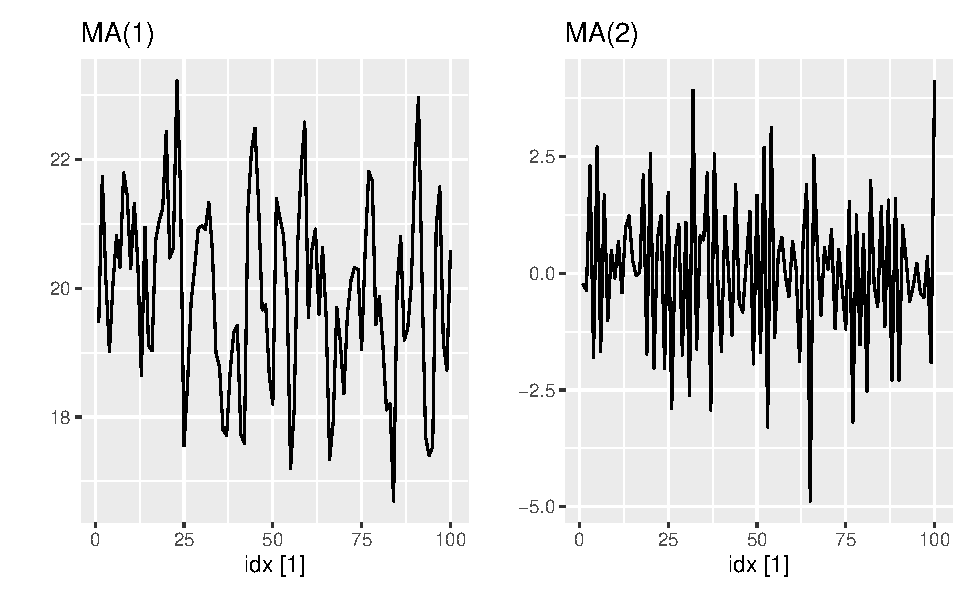
\includegraphics{bookdown-demo_files/figure-latex/maq-1.pdf}

\hypertarget{ma1-model}{%
\subsubsection{MA(1) model}\label{ma1-model}}

\[y_t = 20 + \varepsilon_t + 0.8 \varepsilon_{t-1}\]
\[\varepsilon_t\sim N(0,1),\quad T=100.\]

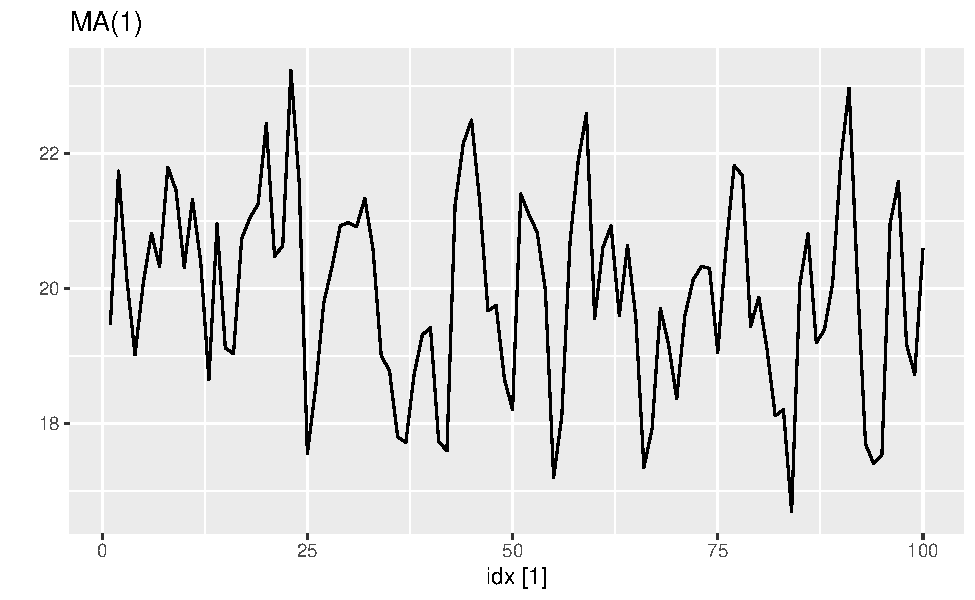
\includegraphics{bookdown-demo_files/figure-latex/unnamed-chunk-9-1.pdf}

\hypertarget{ma2-model}{%
\subsubsection{MA(2) model}\label{ma2-model}}

\[y_t = \varepsilon_t -\varepsilon_{t-1} + 0.8 \varepsilon_{t-2}\]
\[\varepsilon_t\sim N(0,1),\quad T=100.\]

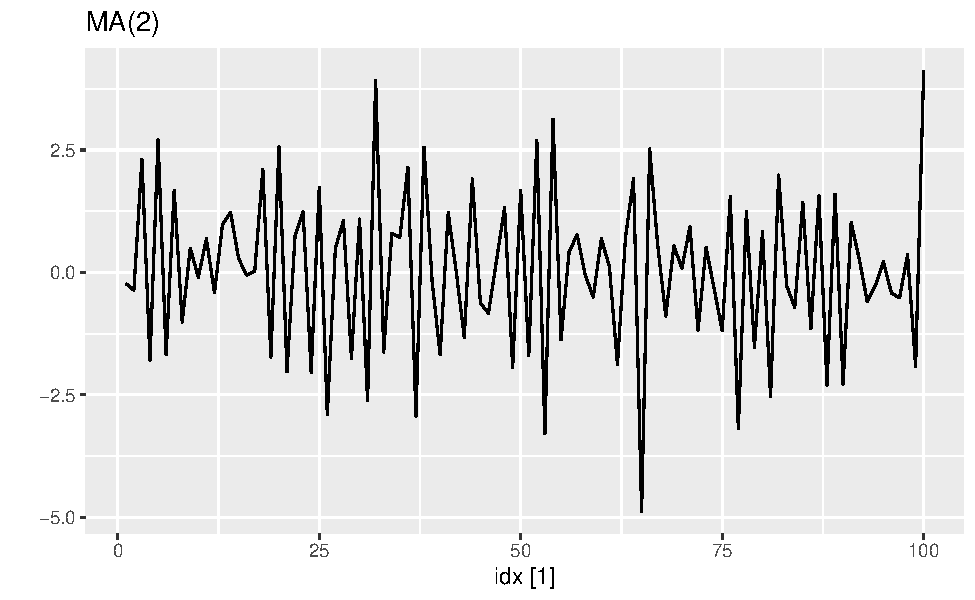
\includegraphics{bookdown-demo_files/figure-latex/unnamed-chunk-10-1.pdf}

\hypertarget{mainfty-models}{%
\subsubsection{\texorpdfstring{MA(\(\infty\)) models}{MA(\textbackslash{}infty) models}}\label{mainfty-models}}

It is possible to write any stationary AR(\(p\)) process as an MA(\(\infty\)) process.

\textbf{Example: AR(1)}
\[y_t = \phi_1y_{t-1} + \varepsilon_t\]
\[= \phi_1(\phi_1y_{t-2} + \varepsilon_{t-1}) + \varepsilon_t\]
\[= \phi_1^2y_{t-2} + \phi_1 \varepsilon_{t-1} + \varepsilon_t\]
\[= \phi_1^3y_{t-3} + \phi_1^2\varepsilon_{t-2} + \phi_1 \varepsilon_{t-1} + \varepsilon_t\]
\[\dots\]

Provided \(-1 < \phi_1 < 1\):
\[y_t = \varepsilon_t + \phi_1 \varepsilon_{t-1} + \phi_1^2 \varepsilon_{t-2} + \phi_1^3 \varepsilon_{t-3} + \cdots\]

\hypertarget{invertibility}{%
\subsection{Invertibility}\label{invertibility}}

\begin{itemize}
\tightlist
\item
  Any MA(\(q\)) process can be written as an AR(\(\infty\)) process if we impose some constraints on the MA parameters.
\item
  Then the MA model is called ``invertible''.
\item
  Invertible models have some mathematical properties that make them easier to use in practice.
\item
  Invertibility of an ARIMA model is equivalent to forecastability of an ETS model.
\end{itemize}

\textbf{General condition for invertibility}

Complex roots of \(1+\theta_1 z + \theta_2 z^2 + \dots + \theta_qz^q\) lie outside the unit circle on the complex plane.

\begin{itemize}
\tightlist
\item
  For \(q=1\): \(-1<\theta_1<1\).
\item
  For \(q=2\):\newline \(-1<\theta_2<1\qquad \theta_2+\theta_1 >-1 \qquad \theta_1 -\theta_2 < 1\).
\item
  More complicated conditions hold for \(q\ge3\).
\item
  Estimation software takes care of this.
\end{itemize}

\hypertarget{arima-models-1}{%
\subsection{ARIMA models}\label{arima-models-1}}

\textbf{Autoregressive Moving Average models:}

\[y_{t} = c + \phi_{1}y_{t - 1} + \cdots + \phi_{p}y_{t - p}\]
\[+ \theta_{1}\varepsilon_{t - 1} + \cdots + \theta_{q}\varepsilon_{t - q} + \varepsilon_{t}\]

\begin{itemize}
\tightlist
\item
  Predictors include both \textbf{lagged values of \(y_t\) and lagged errors.}
\item
  Conditions on coefficients ensure stationarity.
\item
  Conditions on coefficients ensure invertibility.
\end{itemize}

\textbf{Autoregressive Integrated Moving Average models}

\begin{itemize}
\tightlist
\item
  Combine ARMA model with \textbf{differencing}.
\item
  \((1-B)^d y_t\) follows an ARMA model.
\end{itemize}

\textbf{Autoregressive Integrated Moving Average models}

\emph{ARIMA(\(p, d, q\)) model}

\begin{itemize}
\item
  \textbf{AR:} \(p =\) order of the autoregressive part
\item
  \textbf{I:} \(d =\) degree of first differencing involved
\item
  \textbf{MA:} \(q =\) order of the moving average part.

  \begin{itemize}
  \tightlist
  \item
    White noise model: ARIMA(0,0,0)
  \item
    Random walk: ARIMA(0,1,0) with no constant
  \item
    Random walk with drift: ARIMA(0,1,0) with const.
  \item
    AR(\(p\)): ARIMA(\(p\),0,0)
  \item
    MA(\(q\)): ARIMA(0,0,\(q\))
  \end{itemize}
\end{itemize}

\hypertarget{backshift-notation-for-arima}{%
\subsection{Backshift notation for ARIMA}\label{backshift-notation-for-arima}}

\begin{itemize}
\tightlist
\item
  \textbf{ARMA model:}
\end{itemize}

\[y_{t} = c + \phi_{1}By_{t} + \cdots + \phi_pB^py_{t}
           + \varepsilon_{t} + \theta_{1}B\varepsilon_{t} + \cdots + \theta_qB^q\varepsilon_{t}\]

\[\text{or}\quad
      (1-\phi_1B - \cdots - \phi_p B^p) y_t = c + (1 + \theta_1 B + \cdots + \theta_q B^q)\varepsilon_t\]

\textbf{ARIMA(1,1,1) model:}

\[(1 - \phi_{1} B) (1 - B) y_{t} =  c + (1 + \theta_{1} B) \varepsilon_{t}\]

\textbf{NOTE:}

Written out:
\[y_t = c + y_{t-1} + \phi_1 y_{t-1}- \phi_1 y_{t-2} + \theta_1\varepsilon_{t-1} + \varepsilon_t\]

\hypertarget{estimation-and-order-selection}{%
\section{Estimation and order selection}\label{estimation-and-order-selection}}

\hypertarget{maximum-likelihood-estimation}{%
\subsection{Maximum likelihood estimation}\label{maximum-likelihood-estimation}}

Having identified the model order, we need to estimate the parameters \(c\), \(\phi_1,\dots,\phi_p\), \(\theta_1,\dots,\theta_q\).

\begin{itemize}
\tightlist
\item
  MLE is very similar to least squares estimation obtained by minimizing
  \[\sum_{t-1}^T e_t^2\]
\item
  The \texttt{ARIMA()} function allows CLS or MLE estimation.
\item
  Non-linear optimization must be used in either case.
\item
  Different software will give different estimates.
\end{itemize}

\hypertarget{partial-autocorrelations}{%
\subsection{Partial autocorrelations}\label{partial-autocorrelations}}

\textbf{Partial autocorrelations} measure relationship between \(y_{t}\) and \(y_{t - k}\), when the effects of other time lags --- \(1, 2, 3, \dots, k - 1\) --- are removed.

\[\alpha_k = k \text{th partial autocorrelation coefficient}\]

\[= \text{equal to the estimate of } \phi_k \text{ in regression:}\]

\[y_t = c + \phi_1 y_{t-1} + \phi_2 y_{t-2} + \dots + \phi_k y_{t-k}.\]

\begin{itemize}
\tightlist
\item
  Varying number of terms on RHS gives \(\alpha_k\) for different values of \(k\).
\item
  \(\alpha_1=\rho_1\)
\item
  same critical values of \(\pm 1.96/\sqrt{T}\) as for ACF.
\item
  Last significant \(\alpha_k\) indicates the order of an AR model.
\end{itemize}

\hypertarget{example-mink-trapping}{%
\subsubsection{Example: Mink trapping}\label{example-mink-trapping}}

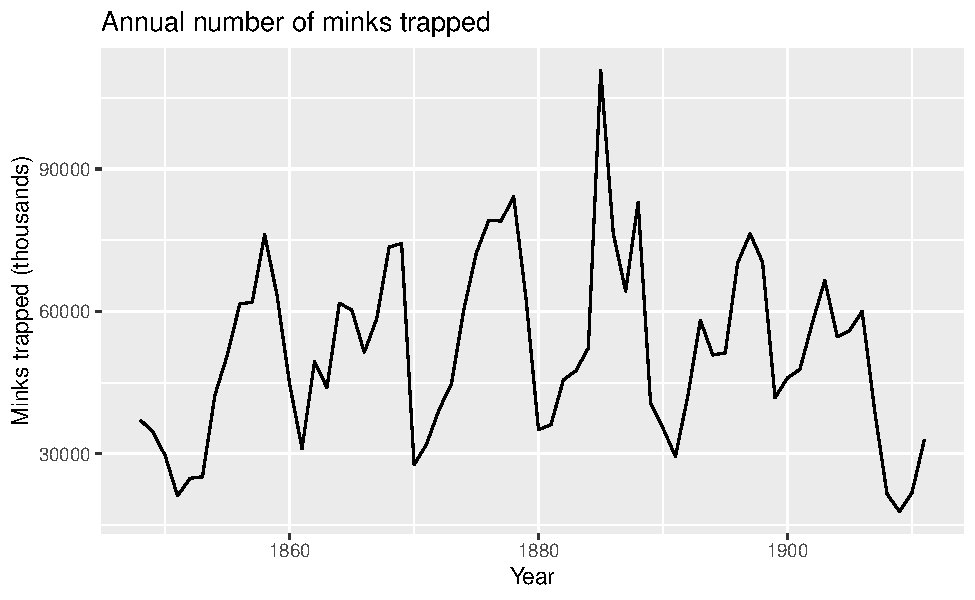
\includegraphics{bookdown-demo_files/figure-latex/unnamed-chunk-11-1.pdf}

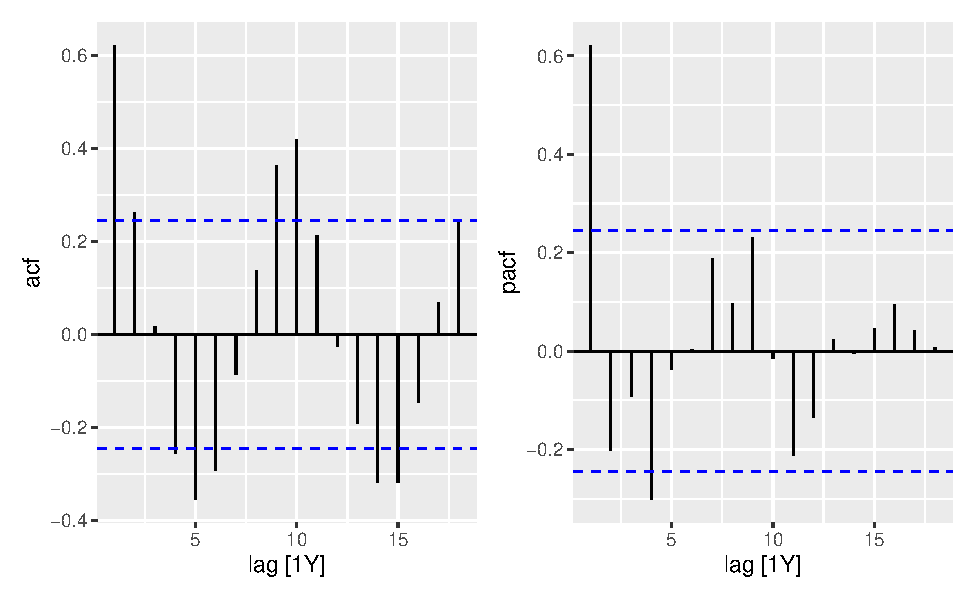
\includegraphics{bookdown-demo_files/figure-latex/unnamed-chunk-12-1.pdf}

\begin{Shaded}
\begin{Highlighting}[]
\NormalTok{mink }\OperatorTok\StringTok{ }\KeywordTok{gg_tsdisplay}\NormalTok{(value, }\DataTypeTok{plot_type=}\StringTok{'partial'}\NormalTok{)}
\end{Highlighting}
\end{Shaded}

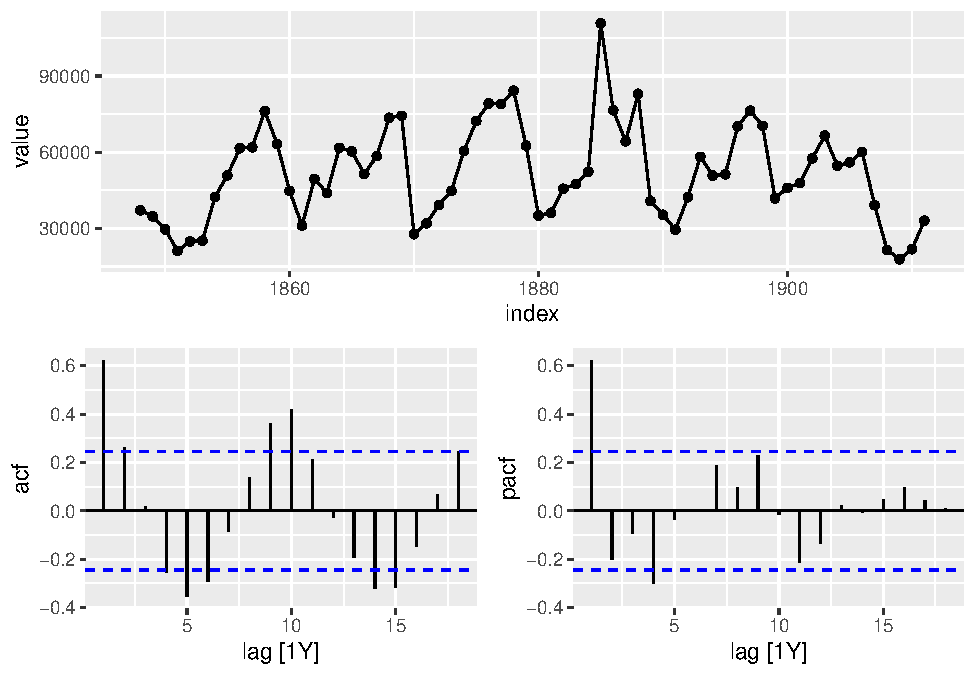
\includegraphics{bookdown-demo_files/figure-latex/unnamed-chunk-13-1.pdf}

\hypertarget{acf-and-pacf-interpretation}{%
\subsection{ACF and PACF interpretation}\label{acf-and-pacf-interpretation}}

\textbf{AR(1)}

\[\rho_k = \phi_1^k\qquad\text{for } k=1,2,\dots;\]

\[\alpha_1 = \phi_1 \qquad\alpha_k = 0\qquad\text{for } k=2,3,\dots.\]

So we have an AR(1) model when

\begin{itemize}
\tightlist
\item
  autocorrelations exponentially decay
\item
  there is a single significant partial autocorrelation.
\end{itemize}

\textbf{AR(\(p\))}

\begin{itemize}
\tightlist
\item
  ACF dies out in an exponential or damped sine-wave manner
\item
  PACF has all zero spikes beyond the \(p\)th spike
\end{itemize}

So we have an AR(\(p\)) model when

\begin{itemize}
\tightlist
\item
  the ACF is exponentially decaying or sinusoidal
\item
  there is a significant spike at lag \(p\) in PACF, but none beyond \(p\)
\end{itemize}

\textbf{MA(1)}

\[\rho_1 = \theta_1\qquad \rho_k = 0\qquad\text{for  }k=2,3,\dots;\]

\[\alpha_k = -(-\theta_1)^k\]

So we have an MA(1) model when

\begin{itemize}
\tightlist
\item
  the PACF is exponentially decaying and
\item
  there is a single significant spike in ACF
\end{itemize}

\textbf{MA(\(q\))}

\begin{itemize}
\tightlist
\item
  PACF dies out in an exponential or damped sine-wave manner
\item
  ACF has all zero spikes beyond the \(q\)th spike
\end{itemize}

So we have an MA(\(q\)) model when

\begin{itemize}
\tightlist
\item
  the PACF is exponentially decaying or sinusoidal
\item
  there is a significant spike at lag \(q\) in ACF, but none beyond \(q\)
\end{itemize}

\hypertarget{information-criteria}{%
\subsection{Information criteria}\label{information-criteria}}

\textbf{Akaike's Information Criterion (AIC)}

\[\text{AIC} = -2 \log(L) + 2(p+q+k+1),\]
where \(L\) is the likelihood of the data, \(k=1\) if \(c\ne0\) and \(k=0\) if \(c=0\).

\textbf{Corrected AIC:}

\[\text{AICc} = \text{AIC} + \displaystyle\frac{2(p+q+k+1)(p+q+k+2)}{T-p-q-k-2}.\]

\textbf{Bayesian Information Criterion:}
\[\text{BIC} = \text{AIC} + [\log(T)-2](p+q+k+1).\]

\begin{itemize}
\tightlist
\item
  Good models are obtained by minimizing either the AIC, AICc or BIC.
\item
  Our preference is to use the AICc.
\end{itemize}

\newpage

\hypertarget{seasonal-arima-models}{%
\section{Seasonal ARIMA models}\label{seasonal-arima-models}}

\begin{longtable}[]{@{}rcc@{}}
\toprule
ARIMA & \(~\underbrace{(p, d, q)}\) & \(\underbrace{(P, D, Q)_{m}}\)\tabularnewline
\midrule
\endhead
& \({\uparrow}\) & \({\uparrow}\)\tabularnewline
& Non-seasonal part & Seasonal part of\tabularnewline
& of the model & of the model\tabularnewline
\bottomrule
\end{longtable}

where \(m =\) number of observations per year.

\textbf{Example:}
ARIMA\((1, 1, 1)(1, 1, 1)_{4}\) model (without constant)

\[(1 - \phi_{1}B)(1 - \Phi_{1}B^{4}) (1 - B) (1 - B^{4})y_{t} ~= ~
(1 + \theta_{1}B) (1 + \Theta_{1}B^{4})\varepsilon_{t}.
\]

\begin{center}
\includegraphics[width=1\linewidth]{bookdown-demo_files/figure-latex/NSbox1-1} \end{center}

All the factors can be multiplied out and the general model
written as follows:

\[y_{t} = (1 + \phi_{1})y_{t - 1} - \phi_1y_{t-2} + (1 + \Phi_{1})y_{t - 4}- (1 + \phi_{1} + \Phi_{1} + \phi_{1}\Phi_{1})y_{t - 5}
 + (\phi_{1} + \phi_{1} \Phi_{1}) y_{t - 6}\]
\[- \Phi_{1} y_{t - 8} + (\Phi_{1} + \phi_{1} \Phi_{1}) y_{t - 9}
  - \phi_{1} \Phi_{1} y_{t - 10} + \varepsilon_{t} + \theta_{1}\varepsilon_{t - 1} + \Theta_{1}\varepsilon_{t - 4} + \theta_{1}\Theta_{1}\varepsilon_{t - 5}.\]

\hypertarget{common-arima-models}{%
\subsection{Common ARIMA models}\label{common-arima-models}}

The US Census Bureau uses the following models most often:\vspace*{0.5cm}

\begin{tabular}{|ll|}
\hline
ARIMA(0,1,1)(0,1,1)$_m$& with log transformation\\
ARIMA(0,1,2)(0,1,1)$_m$& with log transformation\\
ARIMA(2,1,0)(0,1,1)$_m$& with log transformation\\
ARIMA(0,2,2)(0,1,1)$_m$& with log transformation\\
ARIMA(2,1,2)(0,1,1)$_m$& with no transformation\\
\hline
\end{tabular}

\hypertarget{seasonal-arima-models-1}{%
\subsection{Seasonal ARIMA models}\label{seasonal-arima-models-1}}

The seasonal part of an AR or MA model will be seen in the seasonal lags of the PACF and ACF.

\textbf{ARIMA(0,0,0)(0,0,1)\(_{12}\) will show:}

\begin{itemize}
\tightlist
\item
  a spike at lag 12 in the ACF but no other significant spikes.
\item
  The PACF will show exponential decay in the seasonal lags; that is, at lags 12, 24, 36, \dots.
\end{itemize}

\textbf{ARIMA(0,0,0)(1,0,0)\(_{12}\) will show:}

\begin{itemize}
\tightlist
\item
  exponential decay in the seasonal lags of the ACF
\item
  a single significant spike at lag 12 in the PACF.
\end{itemize}

\hypertarget{theoretical-properties-of-the-models}{%
\section{Theoretical properties of the models}\label{theoretical-properties-of-the-models}}

\hypertarget{autoregressive-ar-models}{%
\subsection{Autoregressive (AR) models}\label{autoregressive-ar-models}}

\hypertarget{properties-of-ar1-model}{%
\subsubsection{Properties of AR(1) model}\label{properties-of-ar1-model}}

Consider the following \(AR(1)\) model.

\begin{equation}
  \label{eq:ar}
Y_t=\phi_0+\phi_1Y_{t-1}+\epsilon_{t}
\end{equation}

where \(\varepsilon_t\) is white noise.

\hypertarget{mean}{%
\paragraph{Mean}\label{mean}}

Assuming that the series is weak stationary, we have \(E(Y_t)=\mu\), \(Var(Y_t)=\gamma_0\), and \(Cov(Y_t, Y_{t-k})=\gamma_k\), where \(\mu\) and \(\gamma_0\) are constants. Given that \({\epsilon_t}\) is a white noise, we have \(E(\epsilon_t)=0\). The mean of \(AR(1)\) process can be computed as follows:

\[
\begin{aligned}
  E(Y_t) &= E(\phi_0+\phi_1 Y_{t-1}) \\
         &= E(\phi_0) +E(\phi_1 Y_{t-1}) \\
         &= \phi_0 +\phi_1 E(Y_{t-1}). \\
\end{aligned}
\]
Under the stationarity condition, \(E(Y_t)=E(Y_{t-1})=\mu\). Thus we get

\[\mu = \phi_0+\phi_1\mu.\]

Solving for \(\mu\) yields

\begin{equation}
  \label{eq:2}
E(Y_t)=\mu=\frac{\phi_0}{1-\phi_1}.
\end{equation}

The results has two constraints for \(Y_t\). First, the mean of \(Y_t\) exists if \(\phi_1 \neq 1 .\) The mean of \(Y_t\) is zero if and only if \(\phi_0=0\).

\hypertarget{variance-and-the-stationary-condition-of-ar-1-process}{%
\paragraph{Variance and the stationary condition of AR (1) process}\label{variance-and-the-stationary-condition-of-ar-1-process}}

First take variance of both sides of Equation \eqref{eq:ar}

\[Var(Y_t)=Var(\phi_0+\phi_1 Y_{t-1}+\epsilon_t)\]

The \(Y_{t-1}\) occurred before time \(t\). The \(\epsilon_t\) does not depend on any past observation. Hence, \(cov(Y_{t-1}, \epsilon_t)= 0\). Furthermore, \({\epsilon_t}\) is a white noise. This gives

\[Var(Y_t)=\phi_1^2 Var(Y_{t-1})+\sigma^2.\]

Under the stationarity condition, \(Var(Y_t)=Var(Y_{t-1})\). Hence,

\[Var(Y_t)=\frac{\sigma^2}{1-\phi_1^2}.\]

provided that \(\phi_1^2 < 1\) or \(|\phi_1| < 1\) (The variance of a random variable is bounded and non-negative). The necessary and sufficient condition for the \(AR(1)\) model in Equation \eqref{eq:ar} to be weakly stationary is \(|\phi_1| < 1\). This condition is equivalent to saying that the root of \(1-\phi_1B = 0\) must lie outside the unit circle. This can be explained as below

Using the backshift notation we can write \(AR(1)\) process as

\[Y_t = \phi_0 + \phi_1BY_{t} + \epsilon_t.\]

Then we get

\[(1-\phi_1B)Y_t=\phi_0 + \epsilon_t.\] The \(AR(1)\) process is said to be stationary if the roots of \((1-\phi_1B)=0\) lie outside the unit circle.

\hypertarget{covariance}{%
\paragraph{Covariance}\label{covariance}}

The covariance \(\gamma_k=Cov(Y_t, Y_{t-k})\) is called the lag-\(k\) autocovariance of \(Y_t\). The two main properties of \(\gamma_k\): (a) \(\gamma_0=Var(Y_t)\) and (b) \(\gamma_{-k}=\gamma_{k}\).

The lag-\(k\) autocovariance of \(Y_t\) is

\begin{equation}
  \label{eq:3}
\begin{aligned}
  \gamma_k &= Cov(Y_t, Y_{t-k}) \\
         &= E[(Y_t-\mu)(Y_{t-k}-\mu)] \\
         &= E[Y_tY_{t-k}-Y_t\mu-\mu Y_{t-k} +\mu^2] \\
         &= E(Y_t Y_{t-k}) - \mu^2. \\
\end{aligned}
\end{equation}

Now we have

\begin{equation}
  \label{eq:3}
  E(Y_t Y_{t-k}) = \gamma_k + \mu^2
\end{equation}

\hypertarget{autocorrelation-function-of-an-ar1-process}{%
\paragraph{Autocorrelation function of an AR(1) process}\label{autocorrelation-function-of-an-ar1-process}}

To derive autocorrelation function of an AR(1) process we first multiply both sides of Equation \eqref{eq:ar} by \(Y_{t-k}\) and take expected values:

\[E(Y_tY_{t-k})=\phi_0E(Y_{t-k})+\phi_1 E(Y_{t-1}Y_{t-k})+E(\epsilon_tY_{t-k})\]
Since \(\epsilon_t\) and \(Y_{t-k}\) are independent and using the results in Equation \eqref{eq:3}

\[\gamma_k + \mu^2 = \phi_0 \mu+\phi_1(\gamma_{k-1}+\mu^2)\]

Substituting the results in Equation \eqref{eq:2} to Equation \eqref{eq:3} we get

\begin{equation}
\label{eq:5}
\gamma_k = \phi_1 \gamma_{k-1}.
\end{equation}

The autocorrelation function, \(\rho_k\), is defined as

\[\rho_k = \frac{\gamma_k}{\gamma_0}\].

Setting \(k=1\), we get \(\gamma_1 = \phi_1\gamma_0.\) Hence,

\[\rho_1=\phi_1.\]

Similarly with \(k=2\), \(\gamma_2 = \phi_1 \gamma_1\). Dividing both sides by \(\gamma_0\) and substituting with \(\rho_1=\phi_1\) we get

\[\rho_2=\phi_1^2.\]

Now it is easy to see that in general

\begin{equation}
\label{eq:acfar1}
\rho_k = \frac{\gamma_k}{\gamma_0}=\phi_1^k 
\end{equation}

for \(k=0, 1, 2, 3, ...\).

Since \(|\phi_1| < 1,\) the autocorrelation function is an exponentially decreasing as the number of lags \(k\) increases. There are two features in the ACF of AR(1) process depending on the sign of \(\phi_1\). They are,

\begin{enumerate}
\def\labelenumi{\arabic{enumi}.}
\item
  If \(0 < \phi_1 < 1,\) all correlations are positive.
\item
  if \(-1 < \phi_1 < 0,\) the lag 1 autocorrelation is negative (\(\rho_1=\phi_1\)) and the signs of successive autocorrelations alternate from positive to negative with their magnitudes decreasing exponentially.
\end{enumerate}

\hypertarget{properties-of-ar2-model}{%
\subsubsection{Properties of AR(2) model}\label{properties-of-ar2-model}}

Now consider a second-order autoregressive process (AR(2))

\begin{equation}
  \label{eq:ar2}
Y_t=\phi_0+\phi_1Y_{t-1}+\phi_2Y_{t-2}+\epsilon_t.
\end{equation}

\hypertarget{mean-1}{%
\paragraph{Mean}\label{mean-1}}

\textbf{Question 1:} Using the same technique as that of the AR(1), show that

\[E(Y_t) = \mu = \frac{\phi_0}{1-\phi_1 - \phi_2}\] and the mean of \(Y_t\) exists if \(\phi_1 + \phi_2 \neq 1\).

\hypertarget{variance}{%
\paragraph{Variance}\label{variance}}

\textbf{Question 2:} Show that \[Var(Y_t) = \frac{(1-\phi_2)\sigma^2}{(1+\phi_2)((1+\phi_2)^2-\phi_1^2)}.\]

Here is a guide to the solution

Start with

\[Var(Y_t)=Var(\phi_0+\phi_1Y_{t-1}+\phi_2Y_{t-2}+\epsilon_t)\]

Solve it until you obtain the Eq. (a) as shown below.

\begin{equation}
\tag{a}
\gamma_0 (1-\phi_1^2 - \phi_2^2) = 2\phi_1\phi_2\gamma_1+\sigma^2.
\end{equation}

Next multiply both sides of Equation \eqref{eq:ar2} by \(Y_{t-1}\) and obtain an expression for \(\gamma_1\). Let's call this Eq. (b).

Solve Eq. (a) and (b) for \(\gamma_0.\)

\hypertarget{stationarity-of-ar2-process}{%
\paragraph{Stationarity of AR(2) process}\label{stationarity-of-ar2-process}}

To discuss the stationarity condition of the \(AR(2)\) process we use the roots of the characteristic polynomial. Here is the illustration.

Using the backshift notation we can write \(AR(2)\) process as

\[Y_t = \phi_0 + \phi_1 BY_{t} + \phi_2 B^2 Y_{t} + \epsilon_t.\]

Furthermore, we get

\[(1-\phi_1 B - \phi_2 B^2) Y_t = \phi_0 + \epsilon_t.\]

The \textbf{characteristic polynomial} of \(AR(2)\) process is

\[\Phi(B)=1-\phi_1 B - \phi_2 B^2.\]

and the corresponding \textbf{AR characteristic equation}

\[1-\phi_1 B - \phi_2 B^2=0.\]

For stationarity, the roots of AR characteristic equation must lie outside the unit circle. The two roots of the AR characteristic equation are

\[\frac{\phi_1 \pm \sqrt{\phi_1^2 + 4\phi_2}}{-2\phi_2}\]

Using algebraic manipulation, we can show that these roots will exceed 1 in modulus if and only if simultaneously \(\phi_1 + \phi_2 < 1,\) \(\phi_2-\phi_1 < 1,\) and \(|\phi_2| < 1.\) This is called the stationarity condition of \(AR(2)\) process.

\hypertarget{autocorrelation-function-of-an-ar2-process}{%
\paragraph{Autocorrelation function of an AR(2) process}\label{autocorrelation-function-of-an-ar2-process}}

To derive autocorrelation function of an AR(2) process we first multiply both sides of Equation \eqref{eq:ar2} by \(Y_{t-k}\) and take expected values:

\begin{align}
E(Y_tY_{t-k}) &= E(\phi_0Y_{t-k}+\theta_1Y_{t-1}Y_{t-k}+\theta_2Y_{t-2}Y_{t-k}+\epsilon_tY_{t-k} )\\
&= \phi_0 E(Y_{t-k})+\phi_{1}E(Y_{t-1}Y_{t-k}) + \phi_2 E(Y_{t-2} Y_{t-k}) + E(\epsilon_tY_{t-k}).
\end{align}

Using the independence between \(\epsilon_t\) and \(Y_{t-1}\), \(E(\epsilon_t Y_{t-k})=0\) and the results in Equation \eqref{eq:3} (This is valid for AR(2)) we have

\[\gamma_k + \mu^2 = \phi_0 \mu + \theta_1 (\gamma_{k-1}+\mu^2)+\phi_2 (\gamma_{k-2}+\mu^2).\]

(Note that \(E(X_{t-1}X_{t-k})=E(X_{t-1}X_{(t-1)-(k-1)}=\gamma_{k-1})\))

Solving for \(\gamma_k\) we get

\begin{align}
\label{eq:eq9}
 \gamma_k=\phi_1\gamma_{k-1}+\phi_2\gamma_{k-2}.
\end{align}

By dividing both sides of Equation \eqref{eq:eq9} by \(\gamma_0\), we have

\begin{align}
\label{eq:yule2}
 \rho_k=\phi_1\rho_{k-1}+\phi_2\rho_{k-2}.
\end{align}

for \(k>0\).

Setting \(k=1\) and using \(\rho_0=1\) and \(\rho_{-1}=\rho_1\), we get \textbf{the Yule-Walker equation for \(AR(2)\) process.}

\[\rho_1=\phi_1+\phi_2 \rho_1\] or

\[\rho_1 = \frac{\phi_1}{1-\phi_2}.\]

Similarly, we can show that

\[\rho_2 = \frac{\phi_2(1-\phi_2)+\phi_1^2}{(1-\phi_2)}.\]

\hypertarget{properties-of-arp-model}{%
\subsubsection{Properties of AR(p) model}\label{properties-of-arp-model}}

The \(p\)th order autoregressive model can be written as

\begin{align}
Y_t = \phi_0 + \phi_1Y_{t-1}+\phi_2 Y_{t-2}+ ... + \phi_p Y_{t-p}+\epsilon_t.
\end{align}

The AR characteristic equation is

\[1-\phi_1B-\phi_2B^2-...-\phi_pB^p=0.\]

For stationarity of \(AR(p)\) process, the \(p\) roots of the AR characteristic must lie outside the unit circle.

\hypertarget{mean-2}{%
\paragraph{Mean}\label{mean-2}}

\textbf{Question 3: } Find \(E(Y_t)\) of \(AR(p)\) process.

\hypertarget{variance-1}{%
\paragraph{Variance}\label{variance-1}}

\textbf{Question 4: } Find \(Var(Y_t)\) of \(AR(p)\) process.

\hypertarget{autocorrelation-function-acf-of-an-arp-process}{%
\paragraph{Autocorrelation function (ACF) of an AR(p) process}\label{autocorrelation-function-acf-of-an-arp-process}}

\textbf{Question 5: } Similar to the results in Equation \eqref{eq:yule2} for \(AR(2)\) process, obtain the following recursive relationship for \(AR(p)\).

\begin{align}
\label{eq:yulep}
\rho_k = \phi_1\rho_{k-1}+\phi_2 \rho_{k-2} + ... + \phi_p \rho_{k-p}.
\end{align}

Setting \(k=1, 2, ..., p\) into Equation \eqref{eq:yulep} and using \(\rho_0=1\) and \(\rho_{-k}=\rho_k\), we get the Yule-Walker equations for \(AR(p)\) process

\begin{equation}
  \label{eq:13}
\begin{aligned}
  \rho_1 &= \phi_1+\phi_2 \rho_{1} + ... + \phi_p \rho_{p-1}\\
  \rho_2 &= \phi_1 \rho_1+\phi_2  + ... + \phi_p \rho_{p-2}\\
  ... \\
  \rho_p &= \phi_1 \rho_{p-1} +\phi_2 \rho_{p-2}  + ... + \phi_p \\
\end{aligned}
\end{equation}

The Yule-Walker equations in \eqref{eq:13} can be written in matrix form as below.

\[\left[\begin{array}
{r}
\rho_1  \\
\rho_2  \\
.\\
.\\
.\\
\rho_p
\end{array}\right] = \left[\begin{array}
{rrrrrrr}
1 & \rho_1 & \rho_2 & .&.&.& \rho_{p-1} \\
\rho_1 & 1 & \rho_1 & .&.&.& \rho_{p-2} \\
. & . & . & .&.&.& . \\
. & . & . & .&.&.& . \\
. & . & . & .&.&.& . \\
\rho_{p-1} & \rho_{p-2} & \rho_{p-3} & .&.&.& 1 \\
\end{array}\right] \left[\begin{array}
{r}
\phi_1  \\
\phi_2  \\
.\\
.\\
.\\
\phi_p
\end{array}\right]
\]

or

\[\symbf{{\rho_{p}}}  = \symbf{{P_{p}\phi}}.\]

where,

\[\symbf{\rho_p} = \left[\begin{array}
{r}
\rho_1  \\
\rho_2  \\
.\\
.\\
.\\
\rho_p
\end{array}\right], \mathbf{P_p} = \left[\begin{array}
{rrrrrrr}
1 & \rho_1 & \rho_2 & .&.&.& \rho_{p-1} \\
\rho_1 & 1 & \rho_1 & .&.&.& \rho_{p-2} \\
. & . & . & .&.&.& . \\
. & . & . & .&.&.& . \\
. & . & . & .&.&.& . \\
\rho_{p-1} & \rho_{p-2} & \rho_{p-3} & .&.&.& 1 \\
\end{array}\right], \symbf{{\phi}} = \left[\begin{array}
{r}
\phi_1  \\
\phi_2  \\
.\\
.\\
.\\
\phi_p
\end{array}\right]\]

The parameters can be estimated using

\[\symbf{\phi}=\symbf{P_p^{-1}\rho_p}.\]

\textbf{Question 6:} Obtain the parameters of an \(AR(3)\) process whose first autocorrelations are \(\rho_1=0.9\); \(\rho_2=0.9\); \(\rho_3=0.5\). Is the process stationary?

\hypertarget{the-partial-autocorrelation-function-pacf}{%
\paragraph{The partial autocorrelation function (PACF)}\label{the-partial-autocorrelation-function-pacf}}

Let \(\phi_{kj}\), the \(j\)th coefficient in an \(AR(k)\) model. Then, \(\phi_{kk}\) is the last coefficient. From Equation \eqref{eq:yulep}, the \(\phi_{kj}\) satisfy the set of equations

\begin{equation}
\label{eq:pacf}
\rho_j=\phi_{k1}\rho_{j-1}+...+\phi_{k(k-1)}\rho_{j-k+1}+\phi_{kk}\rho_{j-k},
\end{equation}

for \(j=1, 2, ...k\), leading to the Yule-Walker equations which may be written

\begin{equation}
\label{eq:pacf}
\left[\begin{array}
{r}
\rho_1  \\
\rho_2  \\
.\\
.\\
.\\
\rho_k
\end{array}\right] = \left[\begin{array}
{rrrrrrr}
1 & \rho_1 & \rho_2 & .&.&.& \rho_{k-1} \\
\rho_1 & 1 & \rho_1 & .&.&.& \rho_{k-2} \\
. & . & . & .&.&.& . \\
. & . & . & .&.&.& . \\
. & . & . & .&.&.& . \\
\rho_{k-1} & \rho_{k-2} & \rho_{k-3} & .&.&.& 1 \\
\end{array}\right] \left[\begin{array}
{r}
\phi_{k1}  \\
\phi_{k2}  \\
.\\
.\\
.\\
\phi_{kk}
\end{array}\right]
\end{equation}

or

\[\symbf{\rho_k}=\symbf{P_k\phi_k}.\]

where

\[\symbf{\rho_k} = \left[\begin{array}
{r}
\rho_1  \\
\rho_2  \\
.\\
.\\
.\\
\rho_k
\end{array}\right], \mathbf{P_k} =\left[\begin{array}
{rrrrrrr}
1 & \rho_1 & \rho_2 & .&.&.& \rho_{k-1} \\
\rho_1 & 1 & \rho_1 & .&.&.& \rho_{k-2} \\
. & . & . & .&.&.& . \\
. & . & . & .&.&.& . \\
. & . & . & .&.&.& . \\
\rho_{k-1} & \rho_{k-2} & \rho_{k-3} & .&.&.& 1 \\
\end{array}\right], \symbf{\phi_k} = \left[\begin{array}
{r}
\phi_{k1}  \\
\phi_{k2}  \\
.\\
.\\
.\\
\phi_{kk}
\end{array}\right]\]

For each \(k\), we compute the coefficients \(\phi_{kk}\). Solving the equations for \(k=1, 2, 3...\) successively, we obtain

For \(k=1\),

\begin{equation}
\label{eq:p1}
\phi_{11}=\rho_1.
\end{equation}

For \(k=2\),

\begin{equation}
\label{eq:p2}
\phi_{22}=\frac{\left[\begin{array}
{rr}
1 & \rho_1  \\
\rho_1 & \rho_2  \\
\end{array}\right]}{\left[\begin{array}
{rr}
1 & \rho_1  \\
\rho_1 & 1  \\
\end{array}\right]} = \frac{\rho_2-\rho_1^2}{1-\rho_1^2}
\end{equation}

For \(k=3\),

\begin{equation}
\label{eq:p3}
\phi_{33}=\frac{\left[\begin{array}
{rrr}
1 & \rho_1 & \rho_1  \\
\rho_1 & 1 & \rho_2  \\
\rho_2 & \rho_1 & \rho_3  \\
\end{array}\right]}{\left[\begin{array}
{rrr}
1 & \rho_1 & \rho_2  \\
\rho_1 & 1 & \rho_1  \\
\rho_2 & \rho_1 & 1  \\
\end{array}\right]}
\end{equation}

The quantity \(\phi_{kk}\) is called the partial autocorrelation at lag \(k\) and can be defined as
\[\phi_{kk}=Corr(Y_tY_{t-k}|Y_{t-1}, Y_{t-2},..., Y_{t-k+1}).\]
The partial autocorrelation between \(Y_t\) and \(Y_{t-k}\) is the correlation between \(Y_t\) and \(Y_{t-k}\) after removing the effect of the intermediate variables \(Y_{t-1}, Y_{t-2}, ..., Y_{t-k+1}\).

In general the determinant in the numerator of Equations \eqref{eq:p1}, \eqref{eq:p2} and \eqref{eq:p3} has the same elements as that in the denominator, but replacing the last column with \(\symbf{\rho_k}= (\rho_1, \rho_2,...\rho_k).\)

\hypertarget{pacf-for-ar1-models}{%
\paragraph{PACF for AR(1) models}\label{pacf-for-ar1-models}}

From Equation \eqref{eq:acfar1} we have

\(\rho_k=\phi_1^k\) for \(k=0, 1, 2, 3,...\)

Hence, for \(k=1\), the first partial autocorrelation coefficient is

\[\phi_{11}=\rho_1=\phi_1.\]
From \eqref{eq:p2} for \(k=2\), the second partial autocorrelation coefficient is

\[\phi_{22}=\frac{\rho_2-\rho_1^2}{1-\rho_1^2}=\frac{\phi_1^2-\phi_1^2}{1-\phi_1^2} = 0\].

Similarly, for \(AR(1)\) we can show that \(\phi_{kk}=0\) for all \(k > 1\). Hence, for \(AR(1)\) process the partial autocorrelation is non-zero for lag \(1\) which is the order of the process, but is zero for lags beyond the order 1.

\hypertarget{pacf-for-ar2-model}{%
\paragraph{PACF for AR(2) model}\label{pacf-for-ar2-model}}

\textbf{Question 7:} For \(AR(2)\) process show that \(\phi_{kk}=0\) for all \(k>2\). Sketch the PACF of \(AR(2)\) process.

\hypertarget{pacf-for-arp-model}{%
\paragraph{PACF for AR(P) model}\label{pacf-for-arp-model}}

In general for \(AR(p)\) process, the partial autocorrelation function \(\phi_{kk}\) is non-zero for \(k\) less than or equal to \(p\) (the order of the process) and zero for all \(k\) greater than \(p\). In other words, the partial autocorrelation function of a \(AR(p)\) process has a cut-off after lag \(p\).

\hypertarget{moving-average-ma-models-1}{%
\subsection{Moving average (MA) models}\label{moving-average-ma-models-1}}

We first derive the properties of \(MA(1)\) and \(MA(2)\) models and then give the results for the general \(MA(q)\) model.

\hypertarget{properties-of-ma1-model}{%
\subsubsection{Properties of MA(1) model}\label{properties-of-ma1-model}}

The general form for \(MA(1)\) model is

\begin{equation}
  \label{eq:ma1}
Y_t = \theta_0 + \theta_1 \epsilon_{t-1} + \epsilon_t
\end{equation}

where \(\theta_0\) is a constant and \({\epsilon_t}\) is a white noise series.

\hypertarget{mean-3}{%
\paragraph{Mean}\label{mean-3}}

\textbf{Question 8:} Show that \(E(Y_t) = \theta_0\).

\hypertarget{variance-2}{%
\paragraph{Variance}\label{variance-2}}

\textbf{Question 9:} Show that \(Var(Y_t) = (1+\theta_1^2)\sigma^2\).

We can see both mean and variance are time-invariant. \(MA\) models are finite linear combinations of a white noise sequence. Hence, \(MA\) processes are always weakly stationary.

\hypertarget{autocorrelation-function-of-an-ma1-process}{%
\paragraph{Autocorrelation function of an MA(1) process}\label{autocorrelation-function-of-an-ma1-process}}

\textbf{Method 1}

To obtain the autocorrelation function of \(MA(1)\), we first multiply both sides of Equation \eqref{eq:ma1} by \(Y_{t-k}\) and take the expectation.

\begin{equation}
\label{eq: ma1acfs1}
\begin{aligned}
E[Y_tY_{t-k}] &= E[\theta_0 Y_{t-k} + \theta_1 \epsilon_{t-1} Y_{t-k} + \epsilon_t Y_{t-k}]\\
&= \theta_0 E(Y_{t-k}) + \theta_1 E(\epsilon_{t-1}Y_{t-k}) + E(\epsilon_t Y_{t-k})\\
\end{aligned}
\end{equation}

Using the independence between \(\epsilon_t\) and \(Y_{t-k}\) (future error and past observation) \(E(\epsilon_t Y_{t-k}) = 0\). Now we have

\begin{equation}
\label{eq:ma1acfs2}
E[Y_tY_{t-k}] = \theta_0^2  + \theta_1 E(\epsilon_{t-1}Y_{t-k}) 
\end{equation}

Now let's obtain an expression for \(E[Y_t Y_{t-k}]\).

\begin{equation}
  \label{eq:covma1}
\begin{aligned}
  \gamma_k &= Cov(Y_t, Y_{t-k}) \\
         &= E[(Y_t-\theta_0)(Y_{t-k}-\theta_0)] \\
         &= E[Y_tY_{t-k}-Y_t\theta_0-\theta_0 Y_{t-k} +\theta_0^2] \\
         &= E(Y_t Y_{t-k}) - \theta_0^2. \\
\end{aligned}
\end{equation}

Now we have

\begin{equation}
  \label{eq:covma1}
  E(Y_t Y_{t-k}) = \gamma_k + \theta_0^2.
\end{equation}

Using the Equations \eqref{eq:ma1acfs2} and \eqref{eq:covma1} we have

\begin{equation}
  \label{eq:covma2}
  \gamma_k = \theta_0^2 - \theta_0^2 + \theta_1E(\epsilon_{t-1}Y_{t-k}).
\end{equation}

Now let's consider the case \(k=1\).

\begin{equation}
  \label{eq:covma3}
  \gamma_1 = \theta_0^2 - \theta_0^2 + \theta_1E(\epsilon_{t-1}Y_{t-1})
\end{equation}

Today's error and today's value are dependent. Hence, \(E(\epsilon_{t-1}Y_{t-1}) \neq 0.\) We first need to identify \(E(\epsilon_{t-1}Y_{t-1})\).

\begin{equation}
  \label{eq:covma4}
\begin{aligned}
E(\epsilon_{t-1}Y_{t-1}) &= E(\theta_0 \epsilon_{t-1} + \theta_1 \epsilon_{t-2} \epsilon_{t-1}+ \epsilon_{t-1}^2)\\
\end{aligned}
\end{equation}

Since, \{\(\epsilon_t\)\} is a white noise process \(E(\epsilon_{t-1}) = 0\) and \(E(\epsilon_{t-2} \epsilon_{t-1}) = 0\). Hence, we have

\begin{equation}
  \label{eq:covma5}
\begin{aligned}
E(\epsilon_{t-1}Y_{t-1}) &= E(\epsilon_{t-1}^2)=\sigma^2\\
\end{aligned}
\end{equation}

Substituting \eqref{eq:covma5} in \eqref{eq:covma3} we get

\[\gamma_1=\theta_1\sigma^2\].

Furthermore, \(\gamma_0 = Var(Y_t)= (1+\theta_1^2)\sigma^2\). Hence

\[\rho_1=\frac{\gamma_1}{\gamma_0}=\frac{\theta_1}{1+\theta_1^2}.\]

When \(k=2\), from Equation \eqref{eq:covma3} and \(E(\epsilon_{t-1}Y_{t-2}) = 0\) (future error and past observation) we get \(\gamma_2=0\). Hence \(\rho_2=0\). Similarly, we can show that

\[\gamma_k = \rho_k=0\] for all \(k \geq 2\).

We can see that the ACF of \(MA(1)\) process is zero, beyond the order of 1 of the process.

\textbf{Method 2: By using the definition of covariance}

\begin{equation}
  \label{eq:mtd21}
\begin{aligned}
\gamma_1 = Cov(Y_t, Y_{t-1}) &= Cov(\epsilon_t + \theta_1 \epsilon_{t-1}+ \theta_0, \epsilon_{t-1}+\theta_1 \epsilon_{t-2} + \theta_0)\\
&=Cov(\theta_1 \epsilon_{t-1}, \epsilon_{t-1})\\
&=\theta_1 \sigma^2.
\end{aligned}
\end{equation}

\begin{equation}
  \label{eq:mtd21}
\begin{aligned}
\gamma_2=Cov(Y_t, Y_{t-2}) &= Cov(\epsilon_t + \theta_1 \epsilon_{t-1}+ \theta_0, \epsilon_{t-2}+\theta_1 \epsilon_{t-3} + \theta_0)\\
&=0.
\end{aligned}
\end{equation}

We have \(\gamma_0=\sigma^2(1+\theta_1^2)\), (Using the variance).

Hence

\[\rho_1=\frac{\gamma_1}{\gamma_0}=\frac{\theta_1}{1+\theta_1^2}.\]

Similarly we can show \(\gamma_k=\rho_k=0\) for all \(k \geq 2\).

\hypertarget{properties-of-ma2-model}{%
\subsubsection{Properties of MA(2) model}\label{properties-of-ma2-model}}

An \(MA(2)\) model is in the form

\begin{equation}
  \label{eq:ma2}
Y_t = \theta_0 + \theta_1 \epsilon_{t-1} + \theta_2 \epsilon_{t-2} + \epsilon_t
\end{equation}

where \(\theta_0\) is a constant and \({\epsilon_t}\) is a white noise series.

\hypertarget{mean-4}{%
\paragraph{Mean}\label{mean-4}}

\textbf{Question 10:} Show that \(E(Y_t) = \theta_0.\)

\hypertarget{variance-3}{%
\paragraph{Variance}\label{variance-3}}

\textbf{Question 11: } Show that \(Var(Y_t) = \sigma^2 (1+\theta_1^2 + \theta_2^2).\)

\hypertarget{autocorrelation-function-of-an-ma2-process}{%
\paragraph{Autocorrelation function of an MA(2) process}\label{autocorrelation-function-of-an-ma2-process}}

\textbf{Question 12: }For \(MA(2)\) process show that,

\[\rho_1=\frac{\theta_1(1+\theta_2)}{1+\theta_1^2+\theta_2^2},\]
\[\rho_2 = \frac{\theta_2}{1+\theta_1^2 + \theta_2^2},\]

and \(\rho_k=0\) for all \(k \geq 3.\)

\hypertarget{properties-of-maq-model}{%
\subsubsection{Properties of MA(q) model}\label{properties-of-maq-model}}

\begin{equation}
  \label{eq:ma2}
Y_t = \theta_0 + \theta_1 \epsilon_{t-1} + \theta_2 \epsilon_{t-2} +...+ \theta_q \epsilon_{t-q} +\epsilon_t
\end{equation}

where \(\theta_0\) is a constant and \({\epsilon_t}\) is a white noise series.

\hypertarget{mean-5}{%
\paragraph{Mean}\label{mean-5}}

\textbf{Question 13:} Show that the constant term of an \(MA\) model is the mean of the series (i.e.~\(E(Y_t)=\theta_0\)).

\hypertarget{variance-4}{%
\paragraph{Variance}\label{variance-4}}

\textbf{Question 14:} Show that the variance of an \(MA\) model is
\[Var(Y_t)=(1+\theta_1^2+\theta_2^2+...+\theta_q^2)\sigma^2.\]

\hypertarget{autocorrelation-function-of-an-maq-process}{%
\paragraph{Autocorrelation function of an MA(q) process}\label{autocorrelation-function-of-an-maq-process}}

\textbf{Question 15:} Show that the autocorrelation function of a \(MA(q)\) process is zero, beyond the order of \(q\) of the process. In other words, the autocorrelation function of a moving average process has a cutoff after lag \(q\).

\hypertarget{partial-autocorrelation-function-of-an-maq-process}{%
\paragraph{Partial autocorrelation function of an MA(q) process}\label{partial-autocorrelation-function-of-an-maq-process}}

The partial autocorrelation functions for \(MA(q)\) models behave very much like the autocorrelation functions of \(AR(p)\) models. The PACF of \(MA\) models decays exponentially to zero, rather like ACF for \(AR\) model.

\hypertarget{dual-relation-between-ar-and-ma-process}{%
\subsection{Dual relation between AR and MA process}\label{dual-relation-between-ar-and-ma-process}}

\textbf{Dual relation 1}

\textbf{First we consider the relation AR(p) \textless{}--\textgreater{} MA(}\(\infty\)\textbf{)}

Let \(AR(p)\) be a \textbf{stationary} \(AR\) model with order \(p\). Then,

\[Y_t = \phi_1Y_{t-1}+ \phi_2Y_{t-2}+...+ \phi_pY_{t-p}+\epsilon_t,\]

where \(\epsilon_t \sim WN(0, \sigma^2).\)

Using the backshift operator we can write the \(AR(p)\) model as

\[(1-\phi_1B-\phi_2B^2-...-\phi_pB^P)Y_t=\epsilon_t.\]

Then

\[\phi(B)Y_t=\epsilon_t,\]

where \(\phi(B)=1-\phi_1B-\phi_2B^2-...-\phi_pB^p.\) Furthermore, \(Y_t\) can be written as infinite sum of previous \(\epsilon\)'s as below

\[Y_t = \phi^{-1}(B)\epsilon_t,\]

where \(\phi(B)\psi(B)=1\) and \(\psi(B)=1+\Psi_1B+\psi_2B^2+...\) Then \[Y_t=\psi(B)\epsilon_t.\]
This is a representation of \(MA(\infty)\) process.

\textbf{Next, we consider the relation MA(q) \textless{}--\textgreater{} AR(}\(\infty\)\textbf{)}

Let \(MA(q)\) be \textbf{invertible} moving average process

\[Y_t = \epsilon_t + \theta_t\epsilon_{t-1}+\theta_2\epsilon_{t-2}+...+\theta_p\epsilon_{t-q}.\]

Using the backshift operator we can write the \(MA(q)\) process as

\[Y_t = (1+\theta_1B+\theta_2B^2-...+\theta_qB^q)\epsilon_t.\]

Then,

\[Y_t = \theta(B)\epsilon_t,\]

where \(\theta(B)=1+\theta_1B+\theta_2B^2+...+\theta_1B^q.\) Hence, for an \textbf{invertible} moving average process, \(Y_t\) can be represented as a finite weighted sum of previous error terms, \(\epsilon\). Furthermore, since the process is invertible \(\epsilon_t\) can be represented as an infinite weighted sum of previous \(Y\)'s as below

\[\epsilon_t=\theta^{-1}(B)Y_t,\]
where \(\pi(B)\theta(B)=1\), and \(\pi(B) = 1+\pi_1B+\pi B^2+...\). Hence,

\[\epsilon_t = \pi(B)Y_t.\] This is an representation of a \(AR(\infty)\) process.

\textbf{Dual relation 2}

An \(MA(q)\) process has an ACF function that is zero beyond lag \(q\) and its PACF is decays exponentially to 0. Consequently, an \(AR(p)\) process has an PACF that is zero beyond lag-\(p\), but its ACF decays exponentially to 0.

\textbf{Dual relation 3}

For an \(AR(p)\) process the roots of \(\phi(B)=0\) must lie outside the unit circle to satisfy the condition of stationarity. However, the parameters of the \(AR(p)\) are not required to satisfy any conditions to ensure invertibility. Conversely, the parameters of the \(MA\) process are not required to satisfy any condition to ensure stationarity. However, to ensure the condition of invertibility, the roots of \(\theta(B)=0\) must lie outside the unit circle.

\hypertarget{autoregressive-and-moving-average-arma-models}{%
\subsection{Autoregressive and Moving-average (ARMA) models}\label{autoregressive-and-moving-average-arma-models}}

current value = linear combination of past values + linear combination of past error + current error

The \(ARMA(p, q)\) can be written as

\[Y_t=c+\phi_1 Y_{t-1}+\phi_2 Y_{t-2}+...+\phi_p Y_{t-p}+\theta_1\epsilon_{t-1}+\theta_2\epsilon_{t-2}+...+\theta_q\epsilon_{t-q}+\epsilon_t,\]
where \(\{\epsilon_t\}\) is a white noise process.

Using the back shift operator

\[\phi(B)Y_t=\theta(B)\epsilon_t,\]
where \(\phi(.)\) and \(\theta(.)\) are the \(p\)th and \(q\)th degree polynomials,

\[\phi(B)=1-\phi_1 \epsilon -...-\phi_p \epsilon^p,\]

and
\[\theta(B)=1+\theta_1\epsilon+...+\theta_q\epsilon^q.\]

\hypertarget{stationary-condition}{%
\subsubsection{Stationary condition}\label{stationary-condition}}

Roots of \[\phi(B)=0\] lie outside the unit circle.

\hypertarget{invertible-condition}{%
\subsubsection{Invertible condition}\label{invertible-condition}}

Roots of \[\theta(B)=0\] lie outside the unit circle.

\hypertarget{autocorrelation-function-and-partial-autocorrelation-function}{%
\subsubsection{Autocorrelation function and Partial autocorrelation function}\label{autocorrelation-function-and-partial-autocorrelation-function}}

The ACF of an ARMA model exhibits a pattern similar to that of an AR model. The PACF of ARMA process behaves like the PACF of a MA process. Hence, the ACF and PACF are not informative in determining the order of an ARMA model.

\newpage

\hypertarget{unit-root-tests}{%
\section{Unit root tests}\label{unit-root-tests}}

\begin{itemize}
\tightlist
\item
  Many financial time series are with trending behavior or nonstationarity in the mean.
\item
  Two common trend removal or de-trending procedures

  \begin{itemize}
  \tightlist
  \item
    First differencing (appropriate for \(I(1)\) time series).
  \item
    time-trend regression (appropriate for trend stationary
    \(I(0)\) time series).
  \end{itemize}
\item
  Unit root tests are statistical tests to determine the required order of differencing or whether it should be regressed on deterministic functions of time to render the data stationary.
\end{itemize}

\hypertarget{dickey-fuller-test}{%
\subsection{Dickey-Fuller test}\label{dickey-fuller-test}}

\begin{itemize}
\item
  Consider the model
  \[\Delta y_t = c+ \beta y_{t-1}+\epsilon_{t}\]
\item
  Hypothesis to be tested
  \(H_0: \beta = 0\) and \(H_1: \beta<0\)
\item
  Test statistics = \(\frac{\hat{\beta}}{SE(\hat{\beta})}\)
\end{itemize}

\hypertarget{augmented-dickey-fuller-test}{%
\subsection{Augmented Dickey-Fuller test}\label{augmented-dickey-fuller-test}}

\begin{itemize}
\item
  The Dickey-Fuller Unit Root Test is valid if the time series \(y_t\) is well characterized by an AR(1) model with white noise errors.
\item
  Many financial time series have a more complicated dynamic structures
\item
  The Augmented Dickey-Fuller (ADF) test allows for higher-order autoregressive processes by including \(\Delta y_{t−p}\) in the model.
\item
  The number of lags included in the model should be just sufficient to remove any autocorrelation in errors.
\item
  Consider the model:
  \[\Delta y_t = c+ \beta y_{t-1}+ \alpha_1 \Delta y_{t-1}+\dots + \alpha_p \Delta y_{t-p} +\epsilon_{t}\]
\end{itemize}

\begin{itemize}
\item
  Hypothesis to be tested
  \(H_0: \beta = 0\) and \(H_1: \beta<0\)
\item
  ADF test: null hypothesis is that the data are non-stationary and non-seasonal.
\item
  DF and ADF tests are not suitable when there is a deterministic trend
\item
  Alternative tests:

  \begin{itemize}
  \tightlist
  \item
    Phillips-Perron Unit Root Tests
  \end{itemize}
\item
  The main difference between Phillips-Perron (PP) unit root tests and the ADF tests is in the way they deal with serial correlation and heteroskedasticity in the errors.
\end{itemize}

\hypertarget{stationarity-tests}{%
\subsection{Stationarity Tests}\label{stationarity-tests}}

\begin{itemize}
\tightlist
\item
  The ADF unit root test tests the null hypothesis that a time series \(y_t\) is \(I(1)\).
\item
  In contrast, Stationarity tests are for the null that \(y_t\) is \(I(0)\).
\item
  Kwiatkowski-Phillips-Schmidt-Shin (KPSS) test is the most commonly used stationarity test that tests the null hypothesis that the data are stationary and non-seasonal.
\item
  Other tests available for seasonal data
\end{itemize}

\hypertarget{kwiatkowski-phillips-schmidt-shin-kpss-test}{%
\subsubsection{Kwiatkowski-Phillips-Schmidt-Shin (KPSS) test}\label{kwiatkowski-phillips-schmidt-shin-kpss-test}}

\begin{Shaded}
\begin{Highlighting}[]
\NormalTok{google_}\DecValTok{2018} \OperatorTok
\StringTok{  }\KeywordTok{features}\NormalTok{(Close, unitroot_kpss)}
\end{Highlighting}
\end{Shaded}

\begin{verbatim}
## # A tibble: 1 x 3
##   Symbol kpss_stat kpss_pvalue
##   <chr>      <dbl>       <dbl>
## 1 GOOG       0.573      0.0252
\end{verbatim}

\begin{Shaded}
\begin{Highlighting}[]
\NormalTok{google_}\DecValTok{2018} \OperatorTok
\StringTok{  }\KeywordTok{mutate}\NormalTok{(}\DataTypeTok{diff_close =} \KeywordTok{difference}\NormalTok{(Close)) }\OperatorTok
\StringTok{  }\KeywordTok{features}\NormalTok{(diff_close, unitroot_kpss)}
\end{Highlighting}
\end{Shaded}

\begin{verbatim}
## # A tibble: 1 x 3
##   Symbol kpss_stat kpss_pvalue
##   <chr>      <dbl>       <dbl>
## 1 GOOG      0.0955         0.1
\end{verbatim}

\begin{Shaded}
\begin{Highlighting}[]
\NormalTok{google_}\DecValTok{2018} \OperatorTok
\StringTok{  }\KeywordTok{features}\NormalTok{(Close, unitroot_ndiffs)}
\end{Highlighting}
\end{Shaded}

\begin{verbatim}
## # A tibble: 1 x 2
##   Symbol ndiffs
##   <chr>   <int>
## 1 GOOG        1
\end{verbatim}

\hypertarget{automatically-selecting-differences}{%
\subsubsection{Automatically selecting differences}\label{automatically-selecting-differences}}

STL decomposition: \(y_t = T_t+S_t+R_t\)

Seasonal strength \(F_s = \max\big(0, 1-\frac{\text{Var}(R_t)}{\text{Var}(S_t+R_t)}\big)\)

If \(F_s > 0.64\), do one seasonal difference.

\begin{Shaded}
\begin{Highlighting}[]
\NormalTok{usmelec }\OperatorTok\StringTok{ }\KeywordTok{mutate}\NormalTok{(}\DataTypeTok{log_gen =} \KeywordTok{log}\NormalTok{(Generation)) }\OperatorTok
\StringTok{  }\KeywordTok{features}\NormalTok{(log_gen, }\KeywordTok{list}\NormalTok{(unitroot_nsdiffs, feat_stl))}
\end{Highlighting}
\end{Shaded}

\begin{verbatim}
## # A tibble: 1 x 10
##   nsdiffs trend_strength seasonal_streng~ seasonal_peak_y~
##     <int>          <dbl>            <dbl>            <dbl>
## 1       1          0.994            0.941                7
## # ... with 6 more variables: seasonal_trough_year <dbl>,
## #   spikiness <dbl>, linearity <dbl>, curvature <dbl>,
## #   stl_e_acf1 <dbl>, stl_e_acf10 <dbl>
\end{verbatim}

\begin{Shaded}
\begin{Highlighting}[]
\NormalTok{usmelec }\OperatorTok\StringTok{ }\KeywordTok{mutate}\NormalTok{(}\DataTypeTok{log_gen =} \KeywordTok{log}\NormalTok{(Generation)) }\OperatorTok
\StringTok{  }\KeywordTok{features}\NormalTok{(log_gen, unitroot_nsdiffs)}
\end{Highlighting}
\end{Shaded}

\begin{verbatim}
## # A tibble: 1 x 1
##   nsdiffs
##     <int>
## 1       1
\end{verbatim}

\begin{Shaded}
\begin{Highlighting}[]
\NormalTok{usmelec }\OperatorTok\StringTok{ }\KeywordTok{mutate}\NormalTok{(}\DataTypeTok{d_log_gen =} \KeywordTok{difference}\NormalTok{(}\KeywordTok{log}\NormalTok{(Generation), }\DecValTok{12}\NormalTok{)) }\OperatorTok
\StringTok{  }\KeywordTok{features}\NormalTok{(d_log_gen, unitroot_ndiffs)}
\end{Highlighting}
\end{Shaded}

\begin{verbatim}
## # A tibble: 1 x 1
##   ndiffs
##    <int>
## 1      1
\end{verbatim}

\hypertarget{arima-modelling-in-r}{%
\section{ARIMA modelling in R}\label{arima-modelling-in-r}}

\hypertarget{how-does-arima-work}{%
\subsection{How does ARIMA() work?}\label{how-does-arima-work}}

\textbf{A non-seasonal ARIMA process}

\[\phi(B)(1-B)^dy_{t} = c + \theta(B)\varepsilon_t\]
Need to select appropriate orders: \(p,q, d\)

\textbf{Hyndman and Khandakar (JSS, 2008) algorithm:}

\begin{itemize}
\tightlist
\item
  Select no. differences \(d\) and \(D\) via KPSS test and seasonal strength measure.
\item
  Select \(p,q\) by minimising AICc.
\item
  Use step-wise search to traverse model space.
\end{itemize}

\[\text{AICc} = -2 \log(L) + 2(p+q+k+1)\left[1 +
\frac{(p+q+k+2)}{T-p-q-k-2}\right].\]

where \(L\) is the maximised likelihood fitted to the \emph{differenced} data, \(k=1\) if \(c\neq 0\) and \(k=0\) otherwise.

\textbf{Step1:} Select current model (with smallest AICc) from:\newline
ARIMA\((2,d,2)\)\newline
ARIMA\((0,d,0)\)\newline
ARIMA\((1,d,0)\)\newline
ARIMA\((0,d,1)\)

\textbf{Step 2: Consider variations of current model:}

\begin{itemize}
\tightlist
\item
  vary one of \(p,q,\) from current model by \(\pm1\);
\item
  \(p,q\) both vary from current model by \(\pm1\);
\item
  Include/exclude \(c\) from current model.
\end{itemize}

Model with lowest AICc becomes current model.

\textbf{Repeat Step 2 until no lower AICc can be found.}

\hypertarget{choosing-your-own-model}{%
\subsection{Choosing your own model}\label{choosing-your-own-model}}

\begin{Shaded}
\begin{Highlighting}[]
\NormalTok{web_usage <-}\StringTok{ }\KeywordTok{as_tsibble}\NormalTok{(WWWusage)}
\NormalTok{web_usage }\OperatorTok\StringTok{ }\KeywordTok{gg_tsdisplay}\NormalTok{(value, }\DataTypeTok{plot_type =} \StringTok{'partial'}\NormalTok{)}
\end{Highlighting}
\end{Shaded}

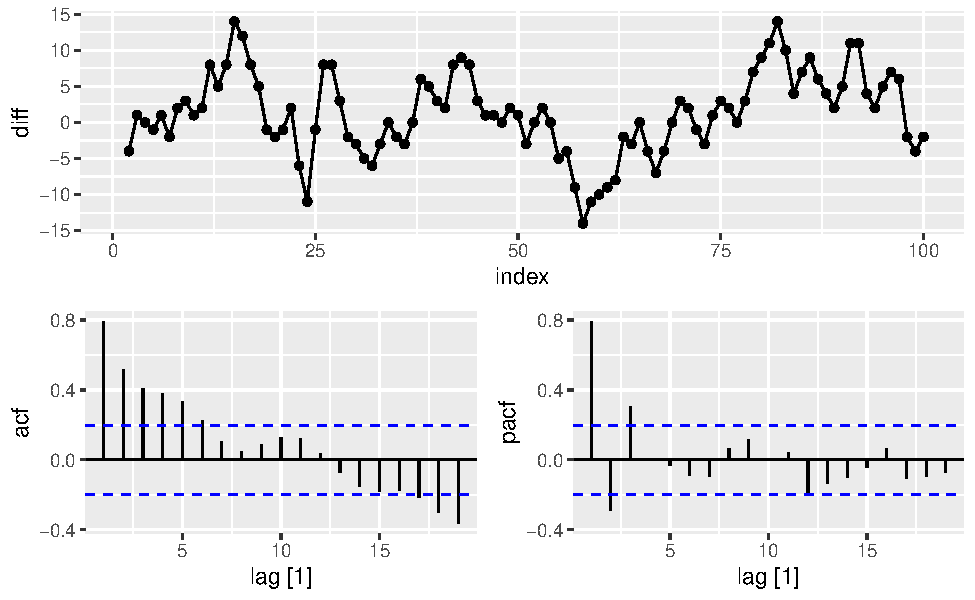
\includegraphics{bookdown-demo_files/figure-latex/unnamed-chunk-19-1.pdf}

\begin{Shaded}
\begin{Highlighting}[]
\NormalTok{web_usage }\OperatorTok\StringTok{ }\KeywordTok{mutate}\NormalTok{(}\DataTypeTok{diff =} \KeywordTok{difference}\NormalTok{(value)) }\OperatorTok
\StringTok{  }\KeywordTok{gg_tsdisplay}\NormalTok{(diff, }\DataTypeTok{plot_type =} \StringTok{'partial'}\NormalTok{)}
\end{Highlighting}
\end{Shaded}

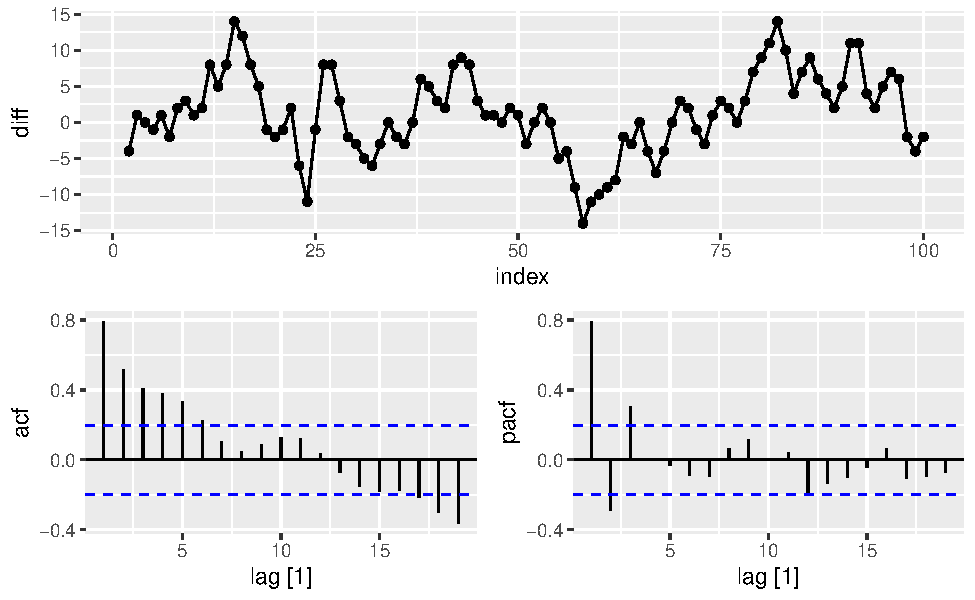
\includegraphics{bookdown-demo_files/figure-latex/unnamed-chunk-20-1.pdf}

\begin{Shaded}
\begin{Highlighting}[]
\NormalTok{fit <-}\StringTok{ }\NormalTok{web_usage }\OperatorTok
\StringTok{  }\KeywordTok{model}\NormalTok{(}\DataTypeTok{arima =} \KeywordTok{ARIMA}\NormalTok{(value }\OperatorTok{~}\StringTok{ }\KeywordTok{pdq}\NormalTok{(}\DecValTok{3}\NormalTok{, }\DecValTok{1}\NormalTok{, }\DecValTok{0}\NormalTok{)))}
\KeywordTok{report}\NormalTok{(fit)}
\end{Highlighting}
\end{Shaded}

\begin{verbatim}
## Series: value 
## Model: ARIMA(3,1,0) 
## 
## Coefficients:
##         ar1      ar2     ar3
##       1.151  -0.6612  0.3407
## s.e.  0.095   0.1353  0.0941
## 
## sigma^2 estimated as 9.656:  log likelihood=-252
## AIC=512   AICc=512.4   BIC=522.4
\end{verbatim}

\begin{Shaded}
\begin{Highlighting}[]
\NormalTok{web_usage }\OperatorTok
\StringTok{  }\KeywordTok{model}\NormalTok{(}\KeywordTok{ARIMA}\NormalTok{(value }\OperatorTok{~}\StringTok{ }\KeywordTok{pdq}\NormalTok{(}\DataTypeTok{d=}\DecValTok{1}\NormalTok{))) }\OperatorTok
\KeywordTok{report}\NormalTok{()}
\end{Highlighting}
\end{Shaded}

\begin{verbatim}
## Series: value 
## Model: ARIMA(1,1,1) 
## 
## Coefficients:
##          ar1     ma1
##       0.6504  0.5256
## s.e.  0.0842  0.0896
## 
## sigma^2 estimated as 9.995:  log likelihood=-254.2
## AIC=514.3   AICc=514.5   BIC=522.1
\end{verbatim}

\begin{Shaded}
\begin{Highlighting}[]
\NormalTok{web_usage }\OperatorTok
\StringTok{  }\KeywordTok{model}\NormalTok{(}\KeywordTok{ARIMA}\NormalTok{(value }\OperatorTok{~}\StringTok{ }\KeywordTok{pdq}\NormalTok{(}\DataTypeTok{d=}\DecValTok{1}\NormalTok{),}
    \DataTypeTok{stepwise =} \OtherTok{FALSE}\NormalTok{, }\DataTypeTok{approximation =} \OtherTok{FALSE}\NormalTok{)) }\OperatorTok
\StringTok{  }\KeywordTok{report}\NormalTok{()}
\end{Highlighting}
\end{Shaded}

\begin{verbatim}
## Series: value 
## Model: ARIMA(3,1,0) 
## 
## Coefficients:
##         ar1      ar2     ar3
##       1.151  -0.6612  0.3407
## s.e.  0.095   0.1353  0.0941
## 
## sigma^2 estimated as 9.656:  log likelihood=-252
## AIC=512   AICc=512.4   BIC=522.4
\end{verbatim}

\begin{Shaded}
\begin{Highlighting}[]
\KeywordTok{gg_tsresiduals}\NormalTok{(fit)}
\end{Highlighting}
\end{Shaded}

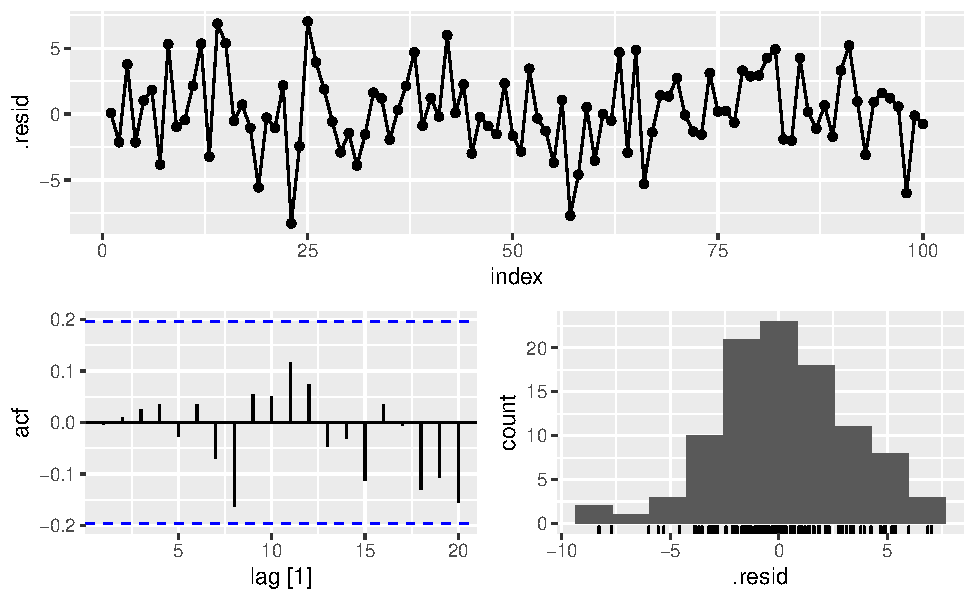
\includegraphics{bookdown-demo_files/figure-latex/unnamed-chunk-23-1.pdf}

\begin{Shaded}
\begin{Highlighting}[]
\KeywordTok{augment}\NormalTok{(fit) }\OperatorTok
\StringTok{  }\KeywordTok{features}\NormalTok{(.resid, ljung_box, }\DataTypeTok{lag =} \DecValTok{10}\NormalTok{, }\DataTypeTok{dof =} \DecValTok{3}\NormalTok{)}
\end{Highlighting}
\end{Shaded}

\begin{verbatim}
## # A tibble: 1 x 3
##   .model lb_stat lb_pvalue
##   <chr>    <dbl>     <dbl>
## 1 arima     4.49     0.722
\end{verbatim}

\begin{Shaded}
\begin{Highlighting}[]
\NormalTok{fit }\OperatorTok\StringTok{ }\KeywordTok{forecast}\NormalTok{(}\DataTypeTok{h =} \DecValTok{10}\NormalTok{) }\OperatorTok
\StringTok{  }\KeywordTok{autoplot}\NormalTok{(web_usage)}
\end{Highlighting}
\end{Shaded}

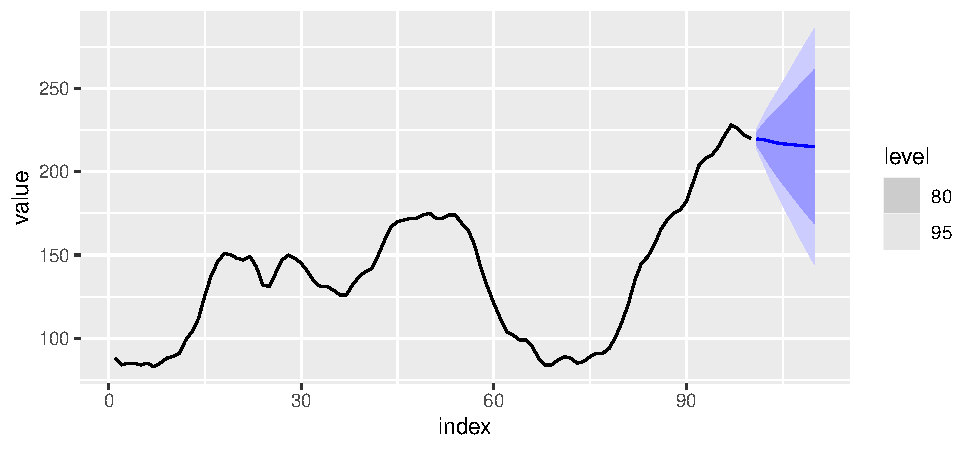
\includegraphics{bookdown-demo_files/figure-latex/unnamed-chunk-25-1.pdf}

\newpage

\hypertarget{modelling-procedure-with-arima}{%
\subsection{\texorpdfstring{Modelling procedure with \texttt{ARIMA()}}{Modelling procedure with ARIMA()}}\label{modelling-procedure-with-arima}}

\begin{enumerate}
\def\labelenumi{\arabic{enumi}.}
\tightlist
\item
  Plot the data. Identify any unusual observations.
\item
  If necessary, transform the data (using a Box-Cox transformation) to stabilize the variance.
\item
  If the data are non-stationary: take first differences of the data until the data are stationary.
\item
  Examine the ACF/PACF: Is an AR(\(p\)) or MA(\(q\)) model appropriate?
\item
  Try your chosen model(s), and use the \(AICc\) to search for a better model.
\item
  Check the residuals from your chosen model by plotting the ACF of the residuals, and doing a portmanteau test of the residuals. If they do not look like white noise, try a modified model.
\item
  Once the residuals look like white noise, calculate forecasts.
\end{enumerate}

\hypertarget{automatic-modelling-procedure-with-arima}{%
\subsection{\texorpdfstring{Automatic modelling procedure with \texttt{ARIMA()}}{Automatic modelling procedure with ARIMA()}}\label{automatic-modelling-procedure-with-arima}}

\begin{enumerate}
\def\labelenumi{\arabic{enumi}.}
\tightlist
\item
  Plot the data. Identify any unusual observations.
\item
  If necessary, transform the data (using a Box-Cox transformation) to stabilize the variance.
\end{enumerate}

\vspace*{0.15cm}

\begin{enumerate}
\def\labelenumi{\arabic{enumi}.}
\setcounter{enumi}{2}
\tightlist
\item
  Use \texttt{ARIMA} to automatically select a model.
\end{enumerate}

\vspace*{0.15cm}

\begin{enumerate}
\def\labelenumi{\arabic{enumi}.}
\setcounter{enumi}{5}
\tightlist
\item
  Check the residuals from your chosen model by plotting the ACF of the residuals, and doing a portmanteau test of the residuals. If they do not look like white noise, try a modified model.
\item
  Once the residuals look like white noise, calculate forecasts.
\end{enumerate}

\hypertarget{example-in-r}{%
\subsection{Example in R}\label{example-in-r}}

\textbf{Seasonally adjusted electrical equipment}

\begin{Shaded}
\begin{Highlighting}[]
\NormalTok{elecequip <-}\StringTok{ }\KeywordTok{as_tsibble}\NormalTok{(fpp2}\OperatorTok{::}\NormalTok{elecequip)}
\NormalTok{dcmp <-}\StringTok{ }\NormalTok{elecequip }\OperatorTok
\StringTok{  }\KeywordTok{model}\NormalTok{(}\KeywordTok{STL}\NormalTok{(value }\OperatorTok{~}\StringTok{ }\KeywordTok{season}\NormalTok{(}\DataTypeTok{window =} \StringTok{"periodic"}\NormalTok{))) }\OperatorTok
\StringTok{  }\KeywordTok{components}\NormalTok{() }\OperatorTok\StringTok{ }\KeywordTok{select}\NormalTok{(}\OperatorTok{-}\NormalTok{.model)}
\NormalTok{dcmp }\OperatorTok\StringTok{ }\NormalTok{as_tsibble }\OperatorTok
\StringTok{  }\KeywordTok{autoplot}\NormalTok{(season_adjust) }\OperatorTok{+}\StringTok{ }\KeywordTok{xlab}\NormalTok{(}\StringTok{"Year"}\NormalTok{) }\OperatorTok{+}
\StringTok{  }\KeywordTok{ylab}\NormalTok{(}\StringTok{"Seasonally adjusted new orders index"}\NormalTok{)}
\end{Highlighting}
\end{Shaded}

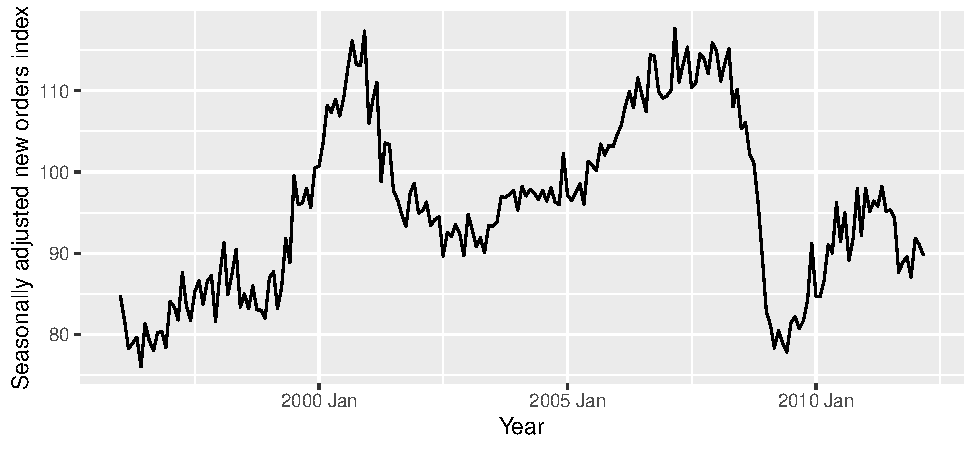
\includegraphics{bookdown-demo_files/figure-latex/ee1-1.pdf}

\begin{Shaded}
\begin{Highlighting}[]
\NormalTok{dcmp }\OperatorTok\StringTok{ }\KeywordTok{mutate}\NormalTok{(}\DataTypeTok{diff =} \KeywordTok{difference}\NormalTok{(season_adjust)) }\OperatorTok
\StringTok{  }\KeywordTok{gg_tsdisplay}\NormalTok{(diff, }\DataTypeTok{plot_type =} \StringTok{'partial'}\NormalTok{)}
\end{Highlighting}
\end{Shaded}

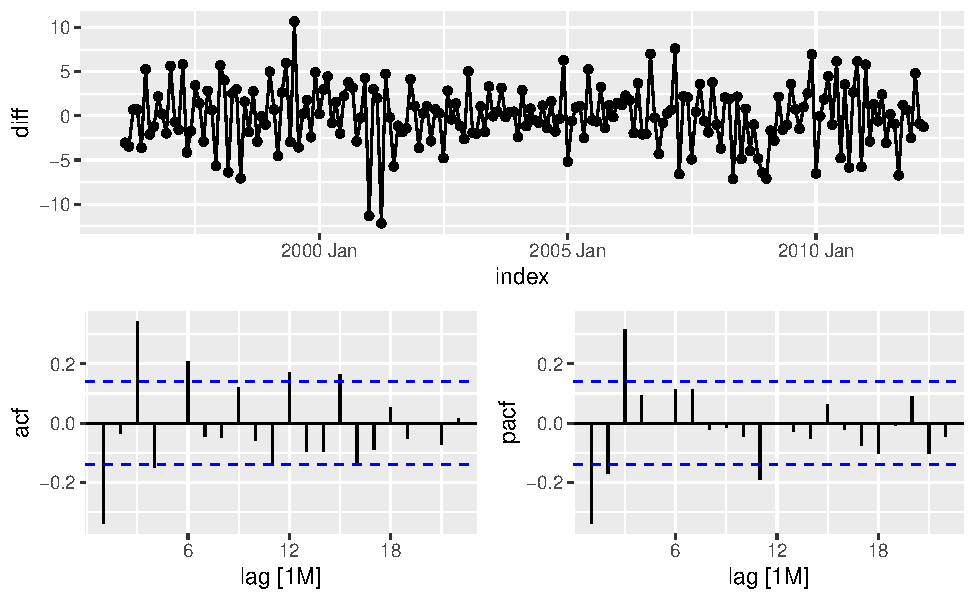
\includegraphics{bookdown-demo_files/figure-latex/ee2-1.pdf}

\begin{Shaded}
\begin{Highlighting}[]
\NormalTok{fit <-}\StringTok{ }\NormalTok{dcmp }\OperatorTok
\StringTok{  }\KeywordTok{model}\NormalTok{(}\DataTypeTok{arima =} \KeywordTok{ARIMA}\NormalTok{(season_adjust))}
\KeywordTok{report}\NormalTok{(fit)}
\end{Highlighting}
\end{Shaded}

\begin{verbatim}
## Series: season_adjust 
## Model: ARIMA(3,1,0) 
## 
## Coefficients:
##           ar1      ar2     ar3
##       -0.3418  -0.0426  0.3185
## s.e.   0.0681   0.0725  0.0682
## 
## sigma^2 estimated as 9.639:  log likelihood=-493.8
## AIC=995.6   AICc=995.8   BIC=1009
\end{verbatim}

\begin{Shaded}
\begin{Highlighting}[]
\NormalTok{fit <-}\StringTok{ }\NormalTok{dcmp }\OperatorTok
\StringTok{  }\KeywordTok{model}\NormalTok{(}\DataTypeTok{arima =} \KeywordTok{ARIMA}\NormalTok{(season_adjust, }\DataTypeTok{approximation=}\OtherTok{FALSE}\NormalTok{))}
\KeywordTok{report}\NormalTok{(fit)}
\end{Highlighting}
\end{Shaded}

\begin{verbatim}
## Series: season_adjust 
## Model: ARIMA(3,1,1) 
## 
## Coefficients:
##          ar1     ar2     ar3      ma1
##       0.0044  0.0916  0.3698  -0.3921
## s.e.  0.2201  0.0984  0.0669   0.2426
## 
## sigma^2 estimated as 9.577:  log likelihood=-492.7
## AIC=995.4   AICc=995.7   BIC=1012
\end{verbatim}

\begin{Shaded}
\begin{Highlighting}[]
\KeywordTok{gg_tsresiduals}\NormalTok{(fit)}
\end{Highlighting}
\end{Shaded}

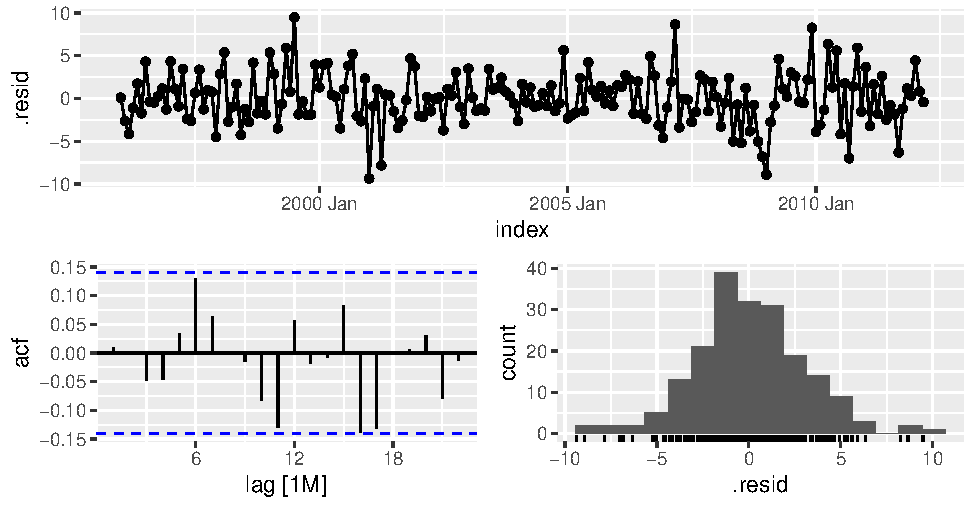
\includegraphics{bookdown-demo_files/figure-latex/unnamed-chunk-28-1.pdf}

\begin{Shaded}
\begin{Highlighting}[]
\KeywordTok{augment}\NormalTok{(fit) }\OperatorTok
\StringTok{  }\KeywordTok{features}\NormalTok{(.resid, ljung_box, }\DataTypeTok{lag =} \DecValTok{24}\NormalTok{, }\DataTypeTok{dof =} \DecValTok{4}\NormalTok{)}
\end{Highlighting}
\end{Shaded}

\begin{verbatim}
## # A tibble: 1 x 3
##   .model lb_stat lb_pvalue
##   <chr>    <dbl>     <dbl>
## 1 arima     24.0     0.241
\end{verbatim}

\begin{Shaded}
\begin{Highlighting}[]
\NormalTok{fit }\OperatorTok\StringTok{ }\NormalTok{forecast }\OperatorTok\StringTok{ }\KeywordTok{autoplot}\NormalTok{(dcmp)}
\end{Highlighting}
\end{Shaded}

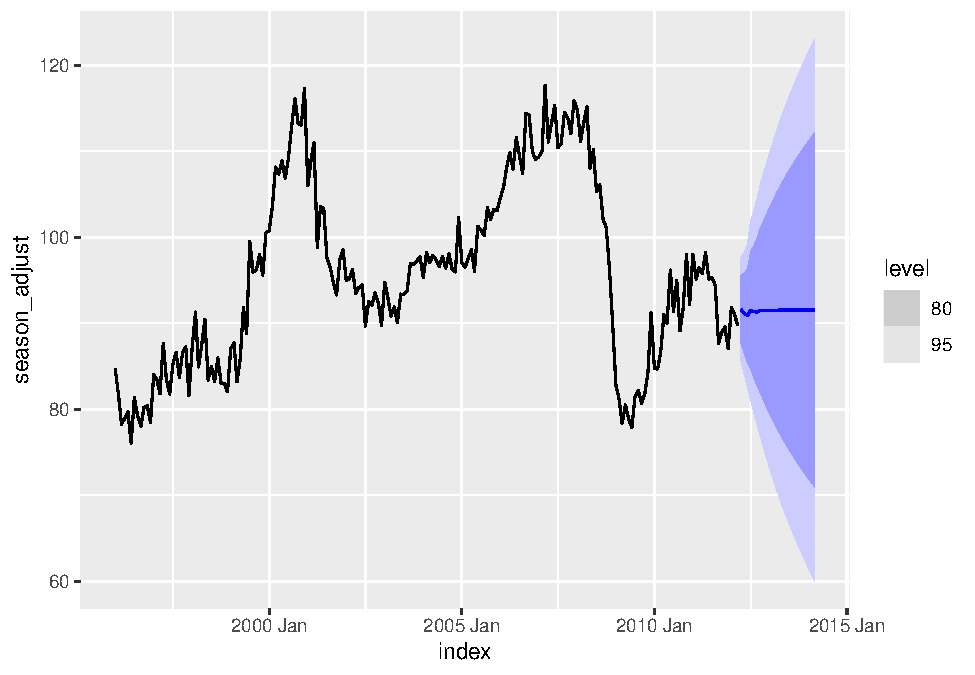
\includegraphics{bookdown-demo_files/figure-latex/unnamed-chunk-30-1.pdf}

\hypertarget{forecasting}{%
\section{Forecasting}\label{forecasting}}

\hypertarget{point-forecasts}{%
\subsection{Point forecasts}\label{point-forecasts}}

\begin{enumerate}
\def\labelenumi{\arabic{enumi}.}
\tightlist
\item
  Rearrange ARIMA equation so \(y_t\) is on LHS.
\item
  Rewrite equation by replacing \(t\) by \(T+h\).
\item
  On RHS, replace future observations by their forecasts, future errors by zero, and past errors by corresponding residuals.
\end{enumerate}

Start with \(h=1\). Repeat for \(h=2,3,\dots\).

\textbf{Example:}

\textbf{ARIMA(3,1,1) forecasts: Step 1}

\[(1-\phi_1B -\phi_2B^2-\phi_3B^3)(1-B) y_t = (1+\theta_1B)\varepsilon_{t},\]

\[[1-(1+\phi_1)B +(\phi_1-\phi_2)B^2 + (\phi_2-\phi_3)B^3 +\phi_3B^4] y_t = (1+\theta_1B)\varepsilon_{t}\]

\[y_t - (1+\phi_1)y_{t-1} +(\phi_1-\phi_2)y_{t-2} + (\phi_2-\phi_3)y_{t-3} \mbox{}+\phi_3y_{t-4} = \varepsilon_t+\theta_1\varepsilon_{t-1}.\]

\[y_t = (1+\phi_1)y_{t-1} -(\phi_1-\phi_2)y_{t-2} - (\phi_2-\phi_3)y_{t-3}\\\mbox{} -\phi_3y_{t-4} + \varepsilon_t+\theta_1\varepsilon_{t-1}.\]

\hypertarget{point-forecasts-h1}{%
\subsubsection{Point forecasts (h=1)}\label{point-forecasts-h1}}

\[y_t = (1+\phi_1)y_{t-1} -(\phi_1-\phi_2)y_{t-2} - (\phi_2-\phi_3)y_{t-3}\\\mbox{} -\phi_3y_{t-4} + \varepsilon_t+\theta_1\varepsilon_{t-1}.\]

\textbf{ARIMA(3,1,1) forecasts: Step 2}

\[y_{T+1} = (1+\phi_1)y_{T} -(\phi_1-\phi_2)y_{T-1} - (\phi_2-\phi_3)y_{T-2}\\\mbox{} -\phi_3y_{T-3} + \varepsilon_{T+1}+\theta_1\varepsilon_{T}.\]

\textbf{ARIMA(3,1,1) forecasts: Step 3}

\[\hat{y}_{T+1|T} = (1+\phi_1)y_{T} -(\phi_1-\phi_2)y_{T-1} - (\phi_2-\phi_3)y_{T-2}\\\mbox{} -\phi_3y_{T-3} + \theta_1 e_{T}.\]

\hypertarget{point-forecasts-h2}{%
\subsubsection{Point forecasts (h=2)}\label{point-forecasts-h2}}

\[y_t = (1+\phi_1)y_{t-1} -(\phi_1-\phi_2)y_{t-2} - (\phi_2-\phi_3)y_{t-3}\\\mbox{} -\phi_3y_{t-4} + \varepsilon_t+\theta_1\varepsilon_{t-1}.\]

\textbf{ARIMA(3,1,1) forecasts: Step 2}

\[y_{T+2} = (1+\phi_1)y_{T+1} -(\phi_1-\phi_2)y_{T} - (\phi_2-\phi_3)y_{T-1}\\\mbox{} -\phi_3y_{T-2} + \varepsilon_{T+2}+\theta_1\varepsilon_{T+1}.\]

\textbf{ARIMA(3,1,1) forecasts: Step 3}

\[\hat{y}_{T+2|T} = (1+\phi_1)\hat{y}_{T+1|T} -(\phi_1-\phi_2)y_{T} - (\phi_2-\phi_3)y_{T-1}\\\mbox{} -\phi_3y_{T-2}.\]

\hypertarget{prediction-intervals}{%
\subsection{Prediction intervals}\label{prediction-intervals}}

\textbf{95\% prediction interval}
\[\hat{y}_{T+h|T} \pm 1.96\sqrt{v_{T+h|T}}\]

where \(v_{T+h|T}\) is estimated forecast variance.

\begin{itemize}
\tightlist
\item
  \(v_{T+1|T}=\hat{\sigma}^2\) for all ARIMA models regardless of parameters and orders.
\item
  Multi-step prediction intervals for \(ARIMA(0,0,q)\)):
\end{itemize}

\[y_t = \varepsilon_t + \sum_{i=1}^q \theta_i \varepsilon_{t-i}.\]

\[\hat{\sigma}_h = \hat{\sigma}^2 \left[ 1 + \sum_{i=1}^{h-1} \theta_i^2\right], \qquad\text{for~} h=2,3,\dots.\]

\begin{itemize}
\tightlist
\item
  AR(1): Rewrite as MA(\(\infty\)) and use above result.
\item
  Other models beyond scope of this subject.
\item
  Prediction intervals \textbf{increase in size with forecast horizon}.
\item
  Prediction intervals can be difficult to calculate by hand
\item
  Calculations assume residuals are \textbf{uncorrelated} and \textbf{normally distributed}.
\item
  Prediction intervals tend to be too narrow.

  \begin{itemize}
  \tightlist
  \item
    the uncertainty in the parameter estimates has not been accounted for.
  \item
    the ARIMA model assumes historical patterns will not change during the forecast period.
  \item
    the ARIMA model assumes uncorrelated future errors.
  \end{itemize}
\end{itemize}

\hypertarget{references}{%
\section{References:}\label{references}}

\begin{itemize}
\item
  Brockwell, P. J., Brockwell, P. J., Davis, R. A., \& Davis, R. A. (2016). Introduction to time series and forecasting. springer.
\item
  Hyndman, R. J., \& Athanasopoulos, G. (2018). Forecasting: principles and practice. OTexts.
\item
  Zivot, E., \& Wang, J. (2006). Unit root tests. Modeling Financial Time Series with S-PLUS®, 111-139.
\end{itemize}

\hypertarget{exponential-smoothing}{%
\chapter{Exponential Smoothing}\label{exponential-smoothing}}

\pagenumbering{arabic}

\hypertarget{introduction}{%
\section{Introduction}\label{introduction}}

\hypertarget{historical-perspective}{%
\subsection{Historical perspective}\label{historical-perspective}}

\begin{itemize}
\tightlist
\item
  Developed in the 1950s and 1960s as methods (algorithms) to produce point forecasts.
\item
  Combine a ``level'', ``trend'' (slope) and ``seasonal'' component to describe a time series.
\item
  The rate of change of the components are controlled by ``smoothing parameters'': \(\alpha\), \(\beta\) and \(\gamma\) respectively.
\item
  Need to choose best values for the smoothing parameters (and initial states).
\item
  Equivalent ETS state space models developed in the 1990s and 2000s.
\end{itemize}

\hypertarget{big-idea-control-the-rate-of-change}{%
\subsection{Big idea: control the rate of change}\label{big-idea-control-the-rate-of-change}}

\(\alpha\) controls the flexibility of the \textbf{level}

\begin{itemize}
\tightlist
\item
  If \(\alpha = 0\), the level never updates (mean)
\item
  If \(\alpha = 1\), the level updates completely (naive)
\end{itemize}

\(\beta\) controls the flexibility of the \textbf{trend}

\begin{itemize}
\tightlist
\item
  If \(\beta = 0\), the trend is linear (regression trend)
\item
  If \(\beta = 1\), the trend updates every observation
\end{itemize}

\(\gamma\) controls the flexibility of the \textbf{seasonality}

\begin{itemize}
\tightlist
\item
  If \(\gamma = 0\), the seasonality is fixed (seasonal means)
\item
  If \(\gamma = 1\), the seasonality updates completely (seasonal naive)
\end{itemize}

\hypertarget{a-model-for-levels-trends-and-seasonalities}{%
\subsection{A model for levels, trends, and seasonalities}\label{a-model-for-levels-trends-and-seasonalities}}

We want a model that captures the level (\(\ell_t\)), trend (\(b_t\)) and seasonality (\(s_t\)).

\textbf{How do we combine these elements?}

\begin{itemize}
\tightlist
\item
  Additively?
\end{itemize}

\[y_t = \ell_{t-1} + b_{t-1} + s_{t-m} + \varepsilon_t\]

\begin{itemize}
\tightlist
\item
  Multiplicatively?
\end{itemize}

\[y_t = \ell_{t-1}b_{t-1}s_{t-m}(1 + \varepsilon_t)\]

\begin{itemize}
\tightlist
\item
  Perhaps a mix of both?
\end{itemize}

\[y_t = (\ell_{t-1} + b_{t-1}) s_{t-m} + \varepsilon_t\]

\textbf{How do the level, trend and seasonal components evolve over time?}

General notation:

\[\text{ETS: } \textbf{E}\text{xponen}\textbf{T}\text{ial}\textbf{ S}\text{moothing}\]

\textbf{E}rror: Additive (\texttt{"A"}) or multiplicative (\texttt{"M"})

\textbf{T}rend: None (\texttt{"N"}), additive (\texttt{"A"}), multiplicative (\texttt{"M"}), or damped (\texttt{"Ad"} or \texttt{"Md"}).

\textbf{S}easonality: None (\texttt{"N"}), additive (\texttt{"A"}) or multiplicative (\texttt{"M"})

\hypertarget{simple-exponential-smoothing}{%
\section{Simple exponential smoothing}\label{simple-exponential-smoothing}}

Time series \(y_1,y_2,\dots,y_T\).

\textbf{Random walk forecasts}
\[\hat{y}_{T+h|T} = y_T\]

\textbf{Average forecasts}

\[\hat{y}_{T+h|T} = \frac1T\sum_{t=1}^T y_t\]

\begin{itemize}
\tightlist
\item
  Want something in between these methods.
\item
  Most recent data should have more weight.
\end{itemize}

\textbf{Forecast equation}

\[\hat{y}_{T+1|T} = \alpha y_T + \alpha(1-\alpha) y_{T-1} + \alpha(1-\alpha)^2 y_{T-2}+ \cdots\]

where \(0 \le \alpha \le1\)

\small

\begin{tabular}{lllll}
\toprule
& \multicolumn{4}{l}{Weights assigned to observations for:}\\
Observation  &   $\alpha = 0.2$   &   $\alpha = 0.4$  &   $\alpha = 0.6$  & $\alpha = 0.8$ \\
\midrule
$y_{T}$      & 0.2         & 0.4          & 0.6         & 0.8\\
$y_{T-1}$    & 0.16        & 0.24         & 0.24        & 0.16\\
$y_{T-2}$    & 0.128       & 0.144        & 0.096       & 0.032\\
$y_{T-3}$    & 0.1024      & 0.0864       & 0.0384      & 0.0064\\
$y_{T-4}$    & $(0.2)(0.8)^4$  & $(0.4)(0.6)^4$   & $(0.6)(0.4)^4$  & $(0.8)(0.2)^4$\\
$y_{T-5}$    & $(0.2)(0.8)^5$  & $(0.4)(0.6)^5$   & $(0.6)(0.4)^5$  & $(0.8)(0.2)^5$\\
\bottomrule
\end{tabular}

\textbf{Component form}

\begin{itemize}
\item
  Forecast equation \(\hat{y}_{t+h|t} = \ell_{t}\)
\item
  Smoothing equation \(\ell_{t} = \alpha y_{t} + (1 - \alpha)\ell_{t-1}\)
\item
  \(\ell_t\) is the level (or the smoothed value) of the series at time t.
\item
  \(\hat{y}_{t+1|t} = \alpha y_t + (1-\alpha) \hat{y}_{t|t-1}\)\newline
  Iterate to get exponentially weighted moving average form.
\end{itemize}

\textbf{Weighted average form}

\[\hat{y}_{T+1|T}=\sum_{j=0}^{T-1} \alpha(1-\alpha)^j y_{T-j}+(1-\alpha)^T \ell_{0}\]

\hypertarget{optimising-smoothing-parameters}{%
\subsection{Optimising smoothing parameters}\label{optimising-smoothing-parameters}}

\begin{itemize}
\tightlist
\item
  Need to choose best values for \(\alpha\) and \(\ell_0\).

  \begin{itemize}
  \tightlist
  \item
    Similarly to regression, choose optimal parameters by minimising SSE:
  \end{itemize}
\end{itemize}

\[\text{SSE}=\sum_{t=1}^T(y_t-\hat{y}_{t|t-1})^2.\]

\begin{itemize}
\item
  Unlike regression there is no closed form solution --- use numerical optimization.
\item
  For Algerian Exports example:

  \begin{itemize}
  \tightlist
  \item
    \(\hat\alpha = 0.8400\)
  \item
    \(\hat\ell_0 = 39.54\)
  \end{itemize}

  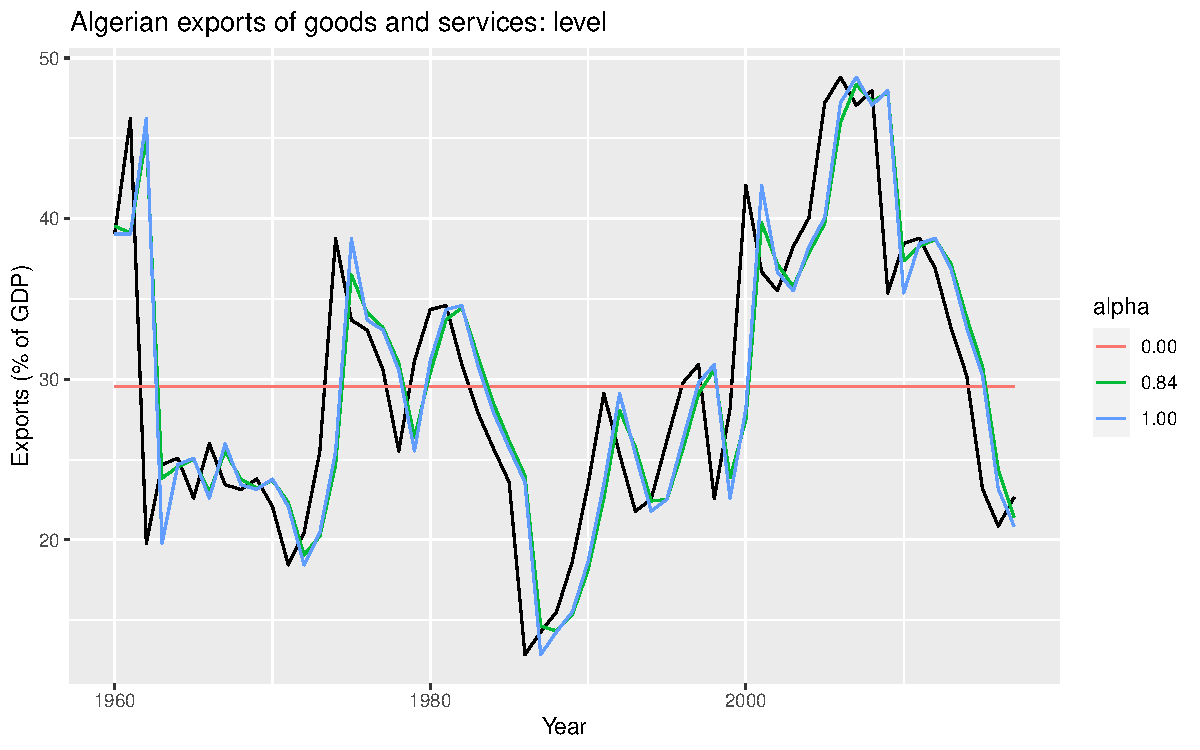
\includegraphics{bookdown-demo_files/figure-latex/alpha-static-1.pdf}
\end{itemize}

\hypertarget{models-and-methods}{%
\subsection{Models and methods}\label{models-and-methods}}

\hypertarget{methods}{%
\subsubsection{Methods}\label{methods}}

\begin{itemize}
\tightlist
\item
  Algorithms that return point forecasts.
\end{itemize}

\hypertarget{models}{%
\subsubsection{Models}\label{models}}

\begin{itemize}
\tightlist
\item
  Generate same point forecasts but can also generate forecast distributions.
\item
  A stochastic (or random) data generating process that can generate an entire forecast distribution.
\item
  Allow for ``proper'' model selection.
\end{itemize}

\hypertarget{etsann-a-model-for-ses}{%
\subsection{ETS(A,N,N): A model for SES}\label{etsann-a-model-for-ses}}

\textbf{Component form}

\begin{itemize}
\item
  Forecast equation: \(\hat{y}_{t+h|t} = \ell_{t}\)
\item
  Smoothing equation: \(\ell_{t} = \alpha y_{t} + (1 - \alpha)\ell_{t-1}\)
\end{itemize}

Forecast error: \(e_t = y_t - \hat{y}_{t|t-1} = y_t - \ell_{t-1}\)

\textbf{Error correction form}

\[y_t = \ell_{t-1} + e_t\]
\[\ell_{t}= \ell_{t-1}+\alpha( y_{t}-\ell_{t-1})\]

\(\ell_{t}=\ell_{t-1}+\alpha e_{t}\)

Specify probability distribution for \(e_t\), we assume \(e_t = \varepsilon_t\sim\text{NID}(0,\sigma^2)\).

\hypertarget{etsann}{%
\subsection{ETS(A,N,N)}\label{etsann}}

\begin{itemize}
\item
  Measurement equation: \(y_t = \ell_{t-1} + \varepsilon_t\)
\item
  State equation: \(\ell_t=\ell_{t-1}+\alpha \varepsilon_t\)
\end{itemize}

where \(\varepsilon_t\sim\text{NID}(0,\sigma^2)\).

\begin{itemize}
\tightlist
\item
  ``innovations'' or ``single source of error'' because equations have the same error process, \(\varepsilon_t\).

  \begin{itemize}
  \tightlist
  \item
    Measurement equation: relationship between observations and states.
  \item
    State equation(s): evolution of the state(s) through time.
  \end{itemize}
\end{itemize}

\hypertarget{etsmnn}{%
\subsection{ETS(M,N,N)}\label{etsmnn}}

SES with multiplicative errors.

\begin{itemize}
\item
  Specify relative errors \(\varepsilon_t=\frac{y_t-\hat{y}_{t|t-1}}{\hat{y}_{t|t-1}}\sim \text{NID}(0,\sigma^2)\)

  \begin{itemize}
  \tightlist
  \item
    Substituting \(\hat{y}_{t|t-1}=\ell_{t-1}\) gives:

    \begin{itemize}
    \tightlist
    \item
      \(y_t = \ell_{t-1}+\ell_{t-1}\varepsilon_t\)
    \item
      \(e_t = y_t - \hat{y}_{t|t-1} = \ell_{t-1}\varepsilon_t\)
    \end{itemize}
  \end{itemize}
\item
  Measurement equation: \(y_t = \ell_{t-1}(1 + \varepsilon_t)\)
\item
  State equation: \(\ell_t=\ell_{t-1}(1+\alpha \varepsilon_t)\)
\item
  Models with additive and multiplicative errors with the same parameters generate the same point forecasts but different prediction intervals.
\end{itemize}

\hypertarget{etsann-specifying-the-model}{%
\subsection{ETS(A,N,N): Specifying the model}\label{etsann-specifying-the-model}}

\begin{Shaded}
\begin{Highlighting}[]
\KeywordTok{ETS}\NormalTok{(y }\OperatorTok{~}\StringTok{ }\KeywordTok{error}\NormalTok{(}\StringTok{"A"}\NormalTok{) }\OperatorTok{+}\StringTok{ }\KeywordTok{trend}\NormalTok{(}\StringTok{"N"}\NormalTok{) }\OperatorTok{+}\StringTok{ }\KeywordTok{season}\NormalTok{(}\StringTok{"N"}\NormalTok{))}
\end{Highlighting}
\end{Shaded}

By default, an optimal value for \(\alpha\) and \(\ell_0\) is used.

\(\alpha\) can be chosen manually in \texttt{trend()}.

\begin{Shaded}
\begin{Highlighting}[]
\KeywordTok{trend}\NormalTok{(}\StringTok{"N"}\NormalTok{, }\DataTypeTok{alpha =} \FloatTok{0.5}\NormalTok{)}
\KeywordTok{trend}\NormalTok{(}\StringTok{"N"}\NormalTok{, }\DataTypeTok{alpha_range =} \KeywordTok{c}\NormalTok{(}\FloatTok{0.2}\NormalTok{, }\FloatTok{0.8}\NormalTok{))}
\end{Highlighting}
\end{Shaded}

\hypertarget{example-algerian-exports}{%
\subsection{Example: Algerian Exports}\label{example-algerian-exports}}

\begin{Shaded}
\begin{Highlighting}[]
\NormalTok{algeria_economy <-}\StringTok{ }\NormalTok{global_economy }\OperatorTok
\StringTok{  }\KeywordTok{filter}\NormalTok{(Country }\OperatorTok{==}\StringTok{ "Algeria"}\NormalTok{)}
\NormalTok{fit <-}\StringTok{ }\NormalTok{algeria_economy }\OperatorTok
\StringTok{  }\KeywordTok{model}\NormalTok{(}\DataTypeTok{ANN =} \KeywordTok{ETS}\NormalTok{(Exports }\OperatorTok{~}\StringTok{ }\KeywordTok{error}\NormalTok{(}\StringTok{"A"}\NormalTok{) }\OperatorTok{+}\StringTok{ }\KeywordTok{trend}\NormalTok{(}\StringTok{"N"}\NormalTok{) }\OperatorTok{+}\StringTok{ }\KeywordTok{season}\NormalTok{(}\StringTok{"N"}\NormalTok{)))}
\KeywordTok{report}\NormalTok{(fit)}
\end{Highlighting}
\end{Shaded}

\begin{verbatim}
## Series: Exports 
## Model: ETS(A,N,N) 
##   Smoothing parameters:
##     alpha = 0.84 
## 
##   Initial states:
##      l
##  39.54
## 
##   sigma^2:  35.63
## 
##   AIC  AICc   BIC 
## 446.7 447.2 452.9
\end{verbatim}

\begin{Shaded}
\begin{Highlighting}[]
\KeywordTok{components}\NormalTok{(fit) }\OperatorTok\StringTok{ }\KeywordTok{autoplot}\NormalTok{()}
\end{Highlighting}
\end{Shaded}

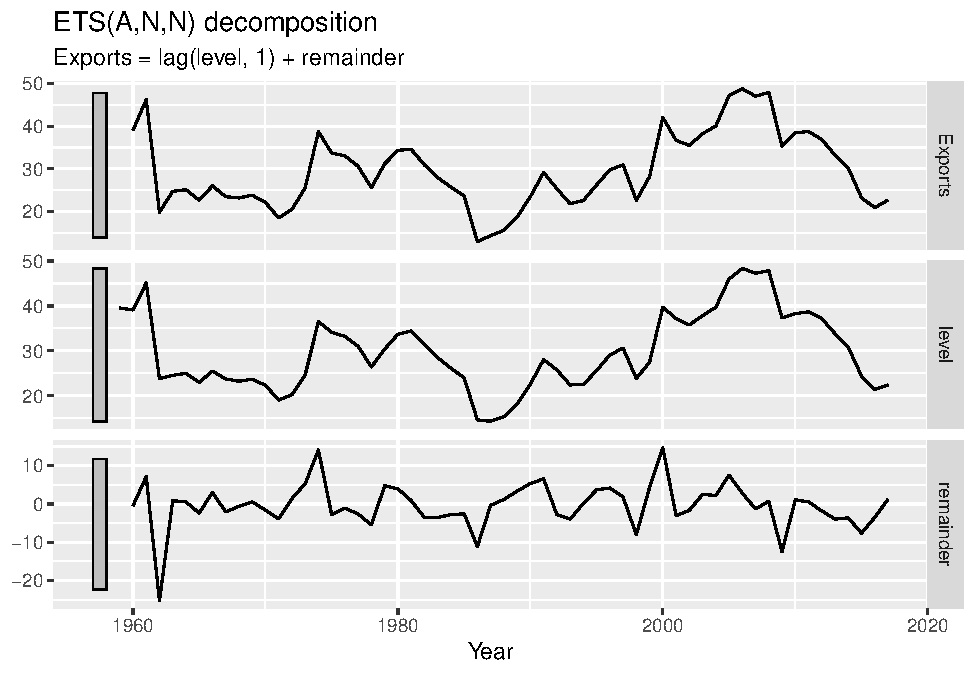
\includegraphics{bookdown-demo_files/figure-latex/ses-cmp0-1.pdf}

\begin{Shaded}
\begin{Highlighting}[]
\KeywordTok{components}\NormalTok{(fit) }\OperatorTok
\StringTok{  }\KeywordTok{left_join}\NormalTok{(}\KeywordTok{fitted}\NormalTok{(fit), }\DataTypeTok{by =} \KeywordTok{c}\NormalTok{(}\StringTok{"Country"}\NormalTok{, }\StringTok{".model"}\NormalTok{, }\StringTok{"Year"}\NormalTok{))}
\end{Highlighting}
\end{Shaded}

\begin{verbatim}
## # A dable:                  59 x 7 [1Y]
## # Key:                      Country, .model [1]
## # ETS(A,N,N) Decomposition: Exports = lag(level, 1) +
## #   remainder
##    Country .model  Year Exports level remainder .fitted
##    <fct>   <chr>  <dbl>   <dbl> <dbl>     <dbl>   <dbl>
##  1 Algeria ANN     1959    NA    39.5    NA        NA  
##  2 Algeria ANN     1960    39.0  39.1    -0.496    39.5
##  3 Algeria ANN     1961    46.2  45.1     7.12     39.1
##  4 Algeria ANN     1962    19.8  23.8   -25.3      45.1
##  5 Algeria ANN     1963    24.7  24.6     0.841    23.8
##  6 Algeria ANN     1964    25.1  25.0     0.534    24.6
##  7 Algeria ANN     1965    22.6  23.0    -2.39     25.0
##  8 Algeria ANN     1966    26.0  25.5     3.00     23.0
##  9 Algeria ANN     1967    23.4  23.8    -2.07     25.5
## 10 Algeria ANN     1968    23.1  23.2    -0.630    23.8
## # ... with 49 more rows
\end{verbatim}

\begin{Shaded}
\begin{Highlighting}[]
\NormalTok{fit }\OperatorTok
\StringTok{  }\KeywordTok{forecast}\NormalTok{(}\DataTypeTok{h =} \DecValTok{5}\NormalTok{) }\OperatorTok
\StringTok{  }\KeywordTok{autoplot}\NormalTok{(algeria_economy) }\OperatorTok{+}
\StringTok{  }\KeywordTok{ylab}\NormalTok{(}\StringTok{"Exports (% of GDP)"}\NormalTok{) }\OperatorTok{+}\StringTok{ }\KeywordTok{xlab}\NormalTok{(}\StringTok{"Year"}\NormalTok{)}
\end{Highlighting}
\end{Shaded}

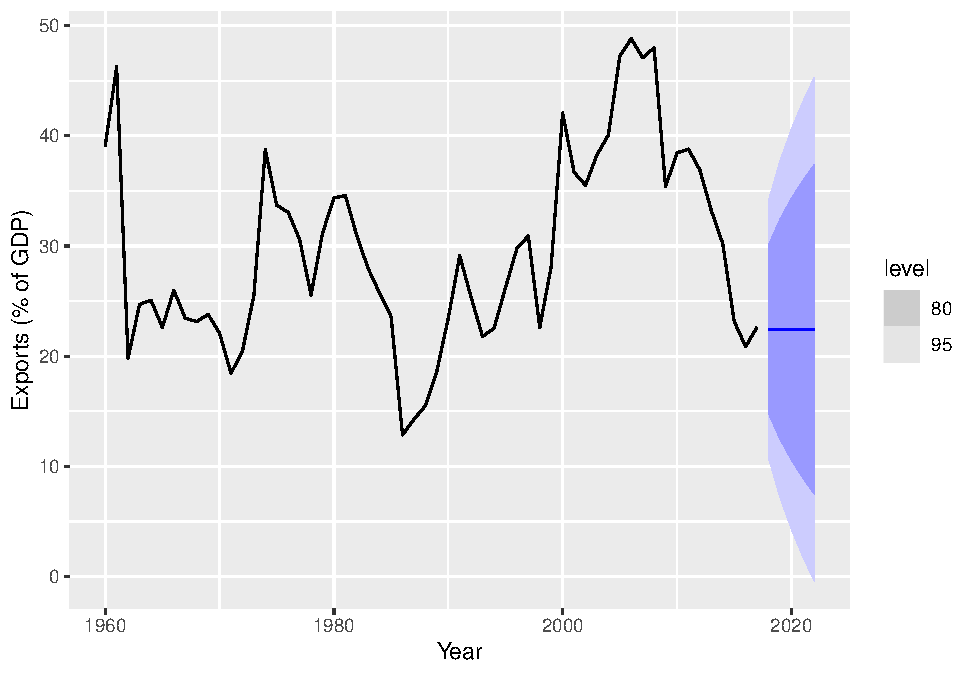
\includegraphics{bookdown-demo_files/figure-latex/ses-fc-1.pdf}

\hypertarget{models-with-trend}{%
\section{Models with trend}\label{models-with-trend}}

\hypertarget{holts-linear-trend}{%
\subsection{Holt's linear trend}\label{holts-linear-trend}}

\textbf{Component form}

\begin{itemize}
\item
  Forecast \(\hat{y}_{t+h|t} = \ell_{t} + hb_{t}\)
\item
  Level \(\ell_{t} = \alpha y_{t} + (1 - \alpha)(\ell_{t-1} + b_{t-1})\)
\item
  Trend \(b_{t} = \beta^*(\ell_{t} - \ell_{t-1}) + (1 -\beta^*)b_{t-1}\)
\item
  Two smoothing parameters \(\alpha\) and \(\beta^*\) (\(0\le\alpha,\beta^*\le1\)).
\item
  \(\ell_t\) level: weighted average between \(y_t\) and one-step ahead forecast for time \(t\), \((\ell_{t-1} + b_{t-1}=\hat{y}_{t|t-1})\)
\item
  \(b_t\) slope: weighted average of \((\ell_{t} - \ell_{t-1})\) and \(b_{t-1}\), current and previous estimate of slope.
\item
  Choose \(\alpha, \beta^*, \ell_0, b_0\) to minimise SSE.
\end{itemize}

\hypertarget{etsaan}{%
\subsection{ETS(A,A,N)}\label{etsaan}}

Holt's linear method with additive errors.

\begin{itemize}
\item
  Assume \(\varepsilon_t=y_t-\ell_{t-1}-b_{t-1} \sim\text{NID}(0,\sigma^2)\).
\item
  Substituting into the error correction equations for Holt's linear method

  \[y_t=\ell_{t-1}+b_{t-1}+\varepsilon_t\]
  \[\ell_t=\ell_{t-1}+b_{t-1}+\alpha \varepsilon_t\]
  \[b_t=b_{t-1}+\alpha\beta^* \varepsilon_t\]
\item
  For simplicity, set \(\beta=\alpha \beta^*\).
\end{itemize}

\hypertarget{exponential-smoothing-trendslope}{%
\subsection{Exponential smoothing: trend/slope}\label{exponential-smoothing-trendslope}}

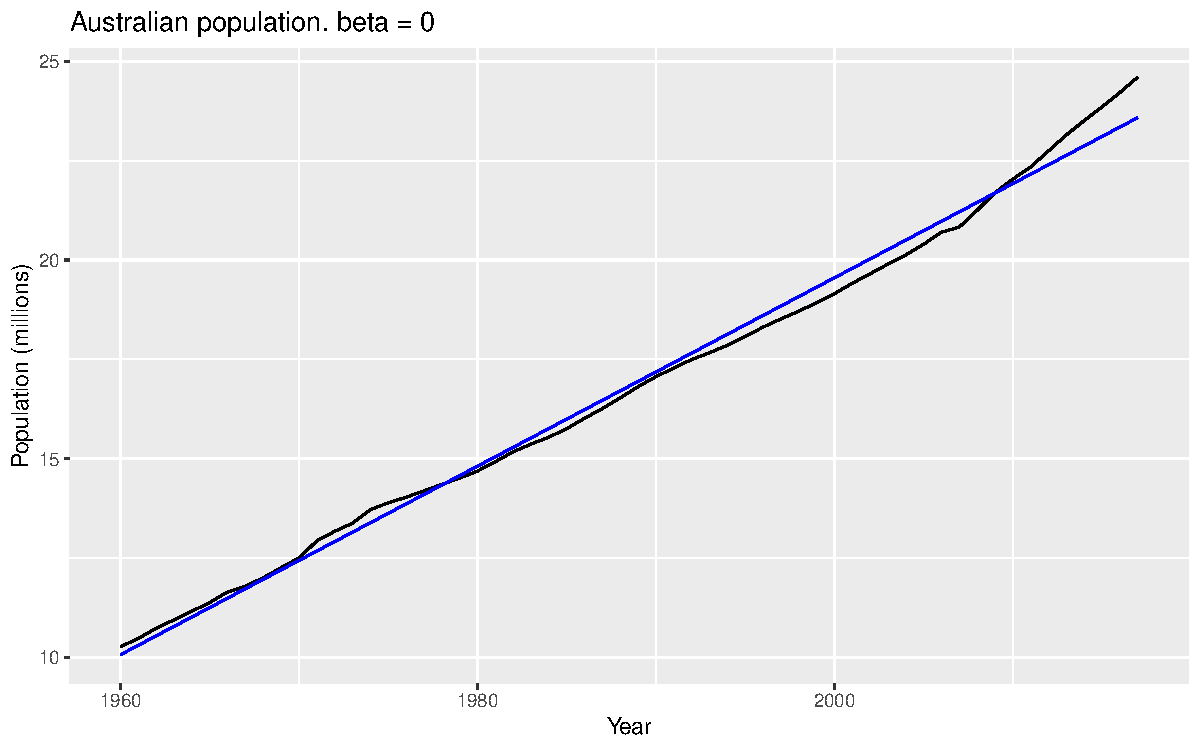
\includegraphics{bookdown-demo_files/figure-latex/beta-static1-1.pdf}

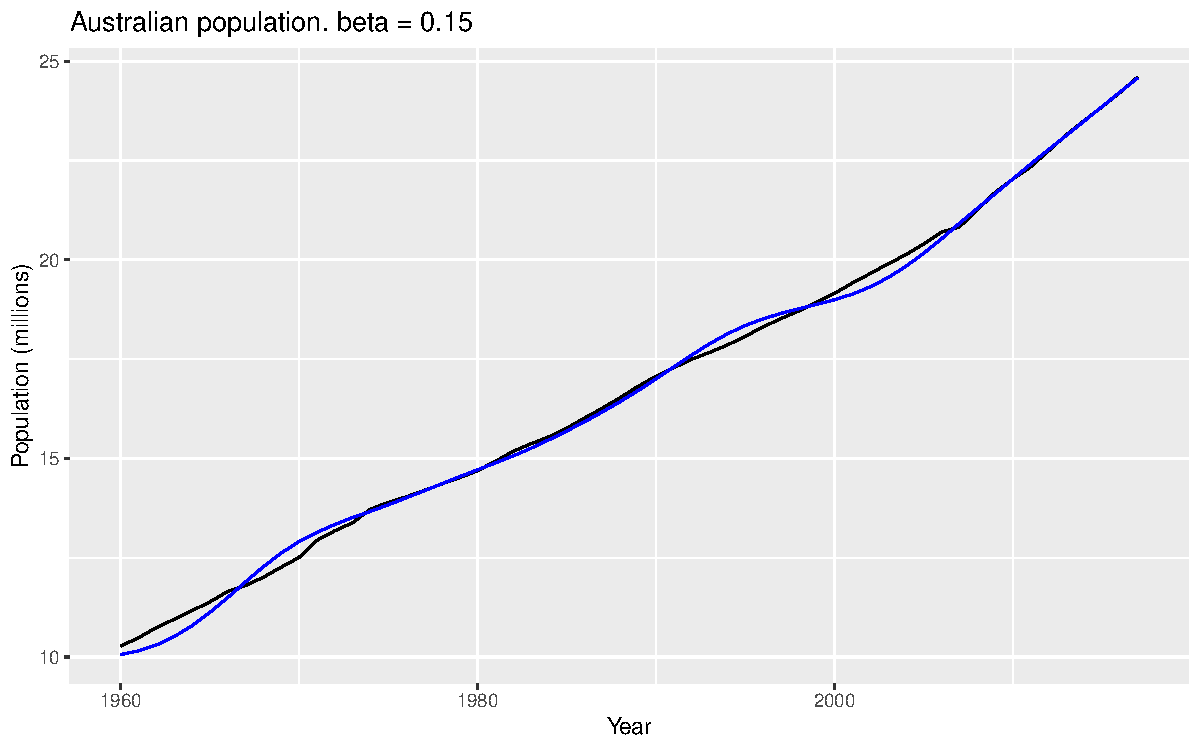
\includegraphics{bookdown-demo_files/figure-latex/beta-static2-1.pdf}

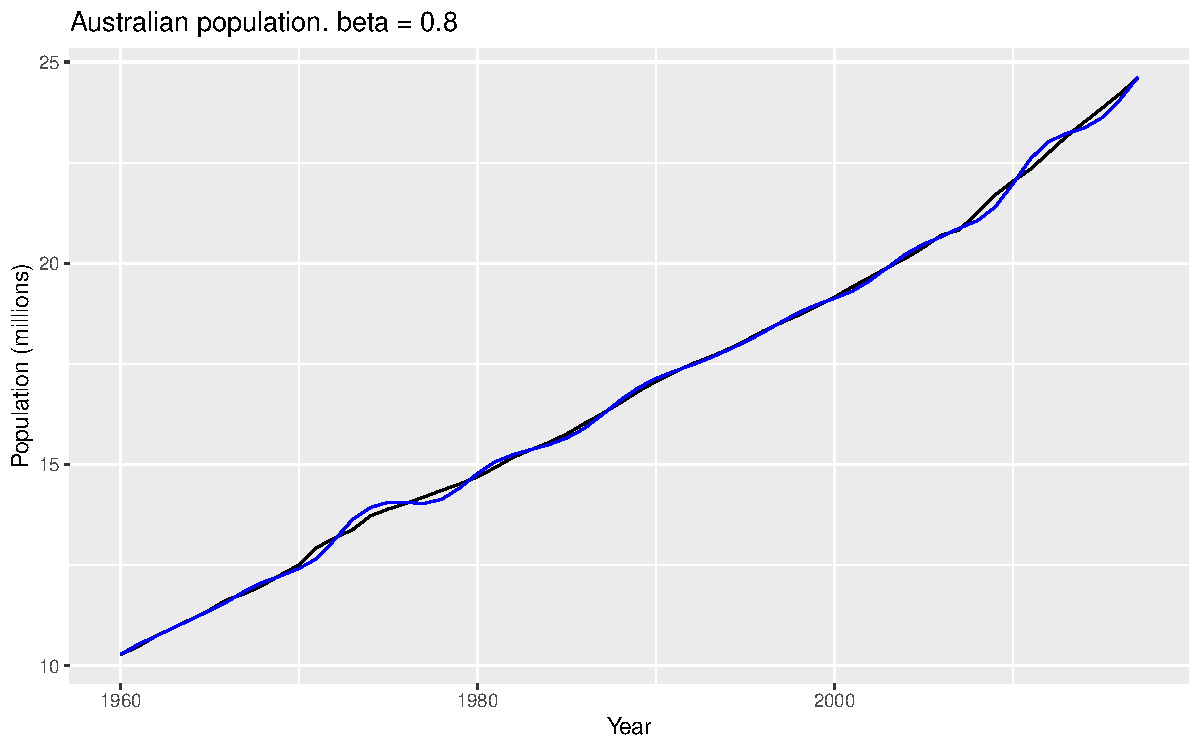
\includegraphics{bookdown-demo_files/figure-latex/beta-static3-1.pdf}

\hypertarget{etsman}{%
\subsection{ETS(M,A,N)}\label{etsman}}

Holt's linear method with multiplicative errors.

\begin{itemize}
\item
  Assume \(\varepsilon_t=\frac{y_t-(\ell_{t-1}+b_{t-1})}{(\ell_{t-1}+b_{t-1})}\)
\item
  Following a similar approach as above, the innovations state space model underlying Holt's linear method with multiplicative errors is specified as

  \[y_t=(\ell_{t-1}+b_{t-1})(1+\varepsilon_t)\]
  \[\ell_t=(\ell_{t-1}+b_{t-1})(1+\alpha \varepsilon_t)\]
  \[b_t=b_{t-1}+\beta(\ell_{t-1}+b_{t-1}) \varepsilon_t\]
\end{itemize}

where again \(\beta=\alpha \beta^*\) and \(\varepsilon_t \sim \text{NID}(0,\sigma^2)\).

\hypertarget{etsaan-specifying-the-model}{%
\subsection{ETS(A,A,N): Specifying the model}\label{etsaan-specifying-the-model}}

\begin{Shaded}
\begin{Highlighting}[]
\KeywordTok{ETS}\NormalTok{(y }\OperatorTok{~}\StringTok{ }\KeywordTok{error}\NormalTok{(}\StringTok{"A"}\NormalTok{) }\OperatorTok{+}\StringTok{ }\KeywordTok{trend}\NormalTok{(}\StringTok{"A"}\NormalTok{) }\OperatorTok{+}\StringTok{ }\KeywordTok{season}\NormalTok{(}\StringTok{"N"}\NormalTok{))}
\end{Highlighting}
\end{Shaded}

By default, optimal values for \(\beta\) and \(b_0\) are used.

\(\beta\) can be chosen manually in \texttt{trend()}.

\begin{Shaded}
\begin{Highlighting}[]
\KeywordTok{trend}\NormalTok{(}\StringTok{"A"}\NormalTok{, }\DataTypeTok{beta =} \FloatTok{0.004}\NormalTok{)}
\KeywordTok{trend}\NormalTok{(}\StringTok{"A"}\NormalTok{, }\DataTypeTok{beta_range =} \KeywordTok{c}\NormalTok{(}\DecValTok{0}\NormalTok{, }\FloatTok{0.1}\NormalTok{))}
\end{Highlighting}
\end{Shaded}

\hypertarget{example-australian-population}{%
\subsection{Example: Australian population}\label{example-australian-population}}

\begin{Shaded}
\begin{Highlighting}[]
\NormalTok{aus_economy <-}\StringTok{ }\NormalTok{global_economy }\OperatorTok\StringTok{ }\KeywordTok{filter}\NormalTok{(Code }\OperatorTok{==}\StringTok{ "AUS"}\NormalTok{) }\OperatorTok
\StringTok{  }\KeywordTok{mutate}\NormalTok{(}\DataTypeTok{Pop =}\NormalTok{ Population}\OperatorTok{/}\FloatTok{1e6}\NormalTok{)}
\NormalTok{fit <-}\StringTok{ }\NormalTok{aus_economy }\OperatorTok
\StringTok{  }\KeywordTok{model}\NormalTok{(}\DataTypeTok{AAN =} \KeywordTok{ETS}\NormalTok{(Pop }\OperatorTok{~}\StringTok{ }\KeywordTok{error}\NormalTok{(}\StringTok{"A"}\NormalTok{) }\OperatorTok{+}\StringTok{ }\KeywordTok{trend}\NormalTok{(}\StringTok{"A"}\NormalTok{) }\OperatorTok{+}\StringTok{ }\KeywordTok{season}\NormalTok{(}\StringTok{"N"}\NormalTok{)))}
\KeywordTok{report}\NormalTok{(fit)}
\end{Highlighting}
\end{Shaded}

\begin{verbatim}
## Series: Pop 
## Model: ETS(A,A,N) 
##   Smoothing parameters:
##     alpha = 0.9999 
##     beta  = 0.3266 
## 
##   Initial states:
##      l      b
##  10.05 0.2225
## 
##   sigma^2:  0.0041
## 
##    AIC   AICc    BIC 
## -76.99 -75.83 -66.68
\end{verbatim}

\begin{Shaded}
\begin{Highlighting}[]
\KeywordTok{components}\NormalTok{(fit) }\OperatorTok\StringTok{ }\KeywordTok{autoplot}\NormalTok{()}
\end{Highlighting}
\end{Shaded}

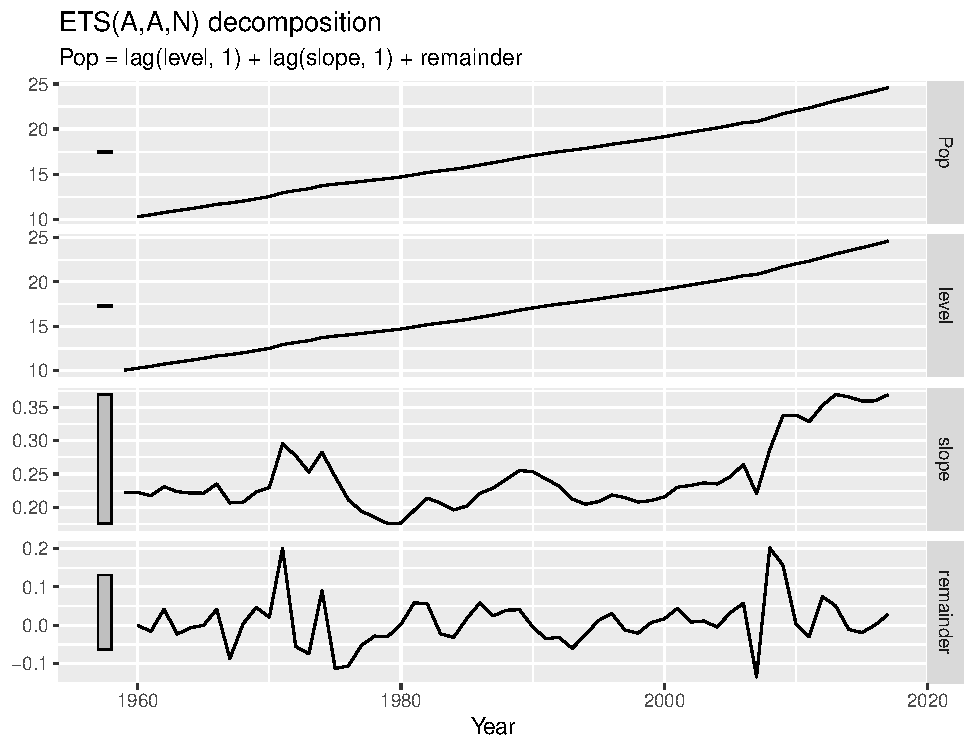
\includegraphics{bookdown-demo_files/figure-latex/holt-cmp-plot-1.pdf}

\begin{Shaded}
\begin{Highlighting}[]
\KeywordTok{components}\NormalTok{(fit) }\OperatorTok
\StringTok{  }\KeywordTok{left_join}\NormalTok{(}\KeywordTok{fitted}\NormalTok{(fit), }\DataTypeTok{by =} \KeywordTok{c}\NormalTok{(}\StringTok{"Country"}\NormalTok{, }\StringTok{".model"}\NormalTok{, }\StringTok{"Year"}\NormalTok{))}
\end{Highlighting}
\end{Shaded}

\begin{verbatim}
## # A dable:                  59 x 8 [1Y]
## # Key:                      Country, .model [1]
## # ETS(A,A,N) Decomposition: Pop = lag(level, 1) +
## #   lag(slope, 1) + remainder
##    Country  .model  Year   Pop level slope remainder .fitted
##    <fct>    <chr>  <dbl> <dbl> <dbl> <dbl>     <dbl>   <dbl>
##  1 Austral~ AAN     1959  NA    10.1 0.222 NA           NA  
##  2 Austral~ AAN     1960  10.3  10.3 0.222 -0.000145    10.3
##  3 Austral~ AAN     1961  10.5  10.5 0.217 -0.0159      10.5
##  4 Austral~ AAN     1962  10.7  10.7 0.231  0.0418      10.7
##  5 Austral~ AAN     1963  11.0  11.0 0.223 -0.0229      11.0
##  6 Austral~ AAN     1964  11.2  11.2 0.221 -0.00641     11.2
##  7 Austral~ AAN     1965  11.4  11.4 0.221 -0.000314    11.4
##  8 Austral~ AAN     1966  11.7  11.7 0.235  0.0418      11.6
##  9 Austral~ AAN     1967  11.8  11.8 0.206 -0.0869      11.9
## 10 Austral~ AAN     1968  12.0  12.0 0.208  0.00350     12.0
## # ... with 49 more rows
\end{verbatim}

\begin{Shaded}
\begin{Highlighting}[]
\NormalTok{fit }\OperatorTok
\StringTok{  }\KeywordTok{forecast}\NormalTok{(}\DataTypeTok{h =} \DecValTok{10}\NormalTok{) }\OperatorTok
\StringTok{  }\KeywordTok{autoplot}\NormalTok{(aus_economy) }\OperatorTok{+}
\StringTok{  }\KeywordTok{ylab}\NormalTok{(}\StringTok{"Population"}\NormalTok{) }\OperatorTok{+}\StringTok{ }\KeywordTok{xlab}\NormalTok{(}\StringTok{"Year"}\NormalTok{)}
\end{Highlighting}
\end{Shaded}

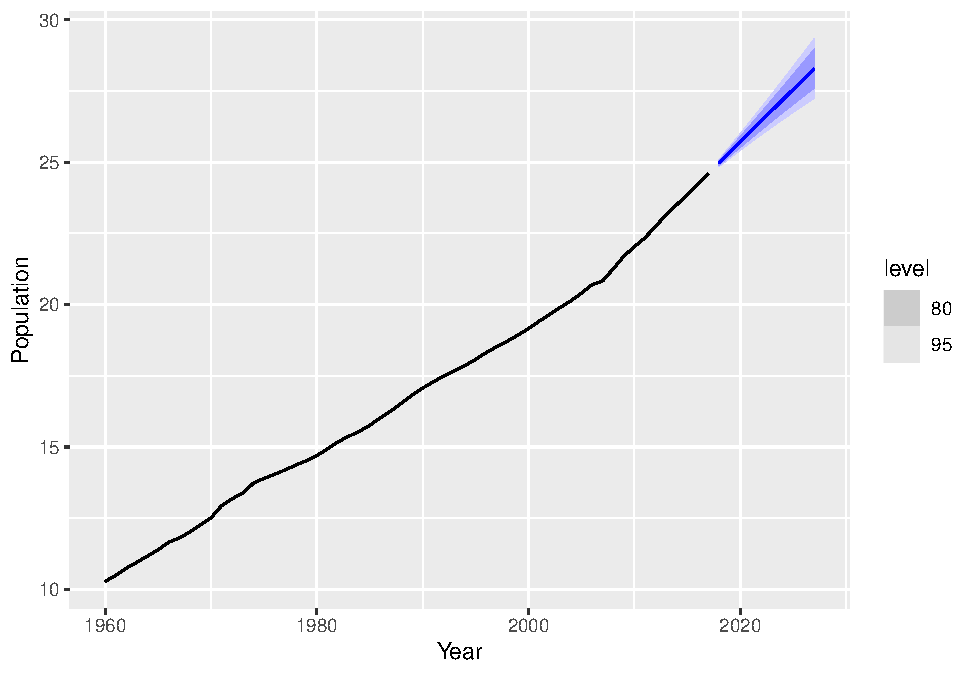
\includegraphics{bookdown-demo_files/figure-latex/holt-fc-1.pdf}

\hypertarget{damped-trend-method}{%
\subsection{Damped trend method}\label{damped-trend-method}}

\textbf{Component form}

\[\hat{y}_{t+h|t} = \ell_{t} + (\phi+\phi^2 + \dots + \phi^{h})b_{t}\]
\[\ell_{t} = \alpha y_{t} + (1 - \alpha)(\ell_{t-1} + \phi b_{t-1})\]
\[b_{t} = \beta^*(\ell_{t} - \ell_{t-1}) + (1 -\beta^*)\phi b_{t-1}.\]

\begin{itemize}
\tightlist
\item
  Damping parameter \(0<\phi<1\).
\item
  If \(\phi=1\), identical to Holt's linear trend.
\item
  As \(h\rightarrow\infty\), \(\hat{y}_{T+h|T}\rightarrow \ell_T+\phi b_T/(1-\phi)\).
\item
  Short-run forecasts trended, long-run forecasts constant.
\end{itemize}

\hypertarget{example-australian-population-1}{%
\subsection{Example: Australian population}\label{example-australian-population-1}}

\begin{itemize}
\tightlist
\item
  Write down the model for ETS(A,\(A_d\),N)
\end{itemize}

\begin{Shaded}
\begin{Highlighting}[]
\NormalTok{aus_economy }\OperatorTok
\StringTok{ }\KeywordTok{model}\NormalTok{(}\DataTypeTok{holt =} \KeywordTok{ETS}\NormalTok{(Pop }\OperatorTok{~}\StringTok{ }\KeywordTok{error}\NormalTok{(}\StringTok{"A"}\NormalTok{) }\OperatorTok{+}\StringTok{ }\KeywordTok{trend}\NormalTok{(}\StringTok{"Ad"}\NormalTok{) }\OperatorTok{+}\StringTok{ }\KeywordTok{season}\NormalTok{(}\StringTok{"N"}\NormalTok{))) }\OperatorTok
\StringTok{ }\KeywordTok{forecast}\NormalTok{(}\DataTypeTok{h =} \DecValTok{20}\NormalTok{) }\OperatorTok
\StringTok{ }\KeywordTok{autoplot}\NormalTok{(aus_economy)}
\end{Highlighting}
\end{Shaded}

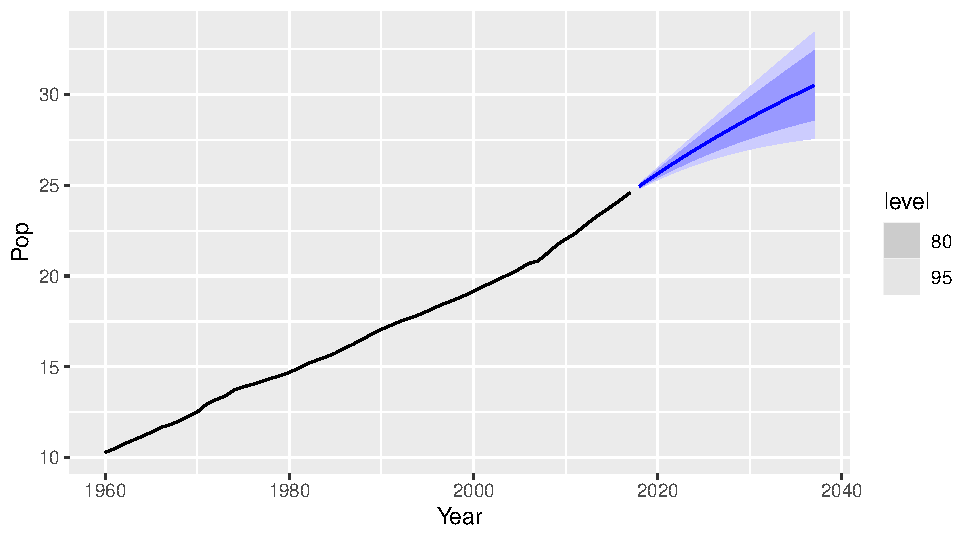
\includegraphics{bookdown-demo_files/figure-latex/unnamed-chunk-31-1.pdf}

\begin{Shaded}
\begin{Highlighting}[]
\NormalTok{fit <-}\StringTok{ }\NormalTok{aus_economy }\OperatorTok
\StringTok{  }\KeywordTok{filter}\NormalTok{(Year }\OperatorTok{<=}\StringTok{ }\DecValTok{2010}\NormalTok{) }\OperatorTok
\StringTok{  }\KeywordTok{model}\NormalTok{(}
    \DataTypeTok{ses =} \KeywordTok{ETS}\NormalTok{(Pop }\OperatorTok{~}\StringTok{ }\KeywordTok{error}\NormalTok{(}\StringTok{"A"}\NormalTok{) }\OperatorTok{+}\StringTok{ }\KeywordTok{trend}\NormalTok{(}\StringTok{"N"}\NormalTok{) }\OperatorTok{+}\StringTok{ }\KeywordTok{season}\NormalTok{(}\StringTok{"N"}\NormalTok{)),}
    \DataTypeTok{holt =} \KeywordTok{ETS}\NormalTok{(Pop }\OperatorTok{~}\StringTok{ }\KeywordTok{error}\NormalTok{(}\StringTok{"A"}\NormalTok{) }\OperatorTok{+}\StringTok{ }\KeywordTok{trend}\NormalTok{(}\StringTok{"A"}\NormalTok{) }\OperatorTok{+}\StringTok{ }\KeywordTok{season}\NormalTok{(}\StringTok{"N"}\NormalTok{)),}
    \DataTypeTok{damped =} \KeywordTok{ETS}\NormalTok{(Pop }\OperatorTok{~}\StringTok{ }\KeywordTok{error}\NormalTok{(}\StringTok{"A"}\NormalTok{) }\OperatorTok{+}\StringTok{ }\KeywordTok{trend}\NormalTok{(}\StringTok{"Ad"}\NormalTok{) }\OperatorTok{+}\StringTok{ }\KeywordTok{season}\NormalTok{(}\StringTok{"N"}\NormalTok{))}
\NormalTok{  )}
\end{Highlighting}
\end{Shaded}

\begin{Shaded}
\begin{Highlighting}[]
\KeywordTok{tidy}\NormalTok{(fit)}
\KeywordTok{accuracy}\NormalTok{(fit)}
\end{Highlighting}
\end{Shaded}

\begin{tabular}{rrrr}
\toprule
term & SES & Linear trend & Damped trend\\
\midrule
alpha & 1.00 & 1.00 & 1.00\\
beta\textasciicircum{}* &  & 0.30 & 0.40\\
phi &  &  & 0.98\\
l\_0 & 10.28 & 10.05 & 10.04\\
b\_0 &  & 0.22 & 0.25\\
\addlinespace
Training RMSE & 0.24 & 0.06 & 0.07\\
Test RMSE & 1.63 & 0.15 & 0.21\\
Test MASE & 6.18 & 0.55 & 0.75\\
Test MAPE & 6.09 & 0.55 & 0.74\\
Test MAE & 1.45 & 0.13 & 0.18\\
\bottomrule
\end{tabular}

\hypertarget{models-with-seasonality}{%
\section{Models with seasonality}\label{models-with-seasonality}}

\hypertarget{holt-winters-additive-method}{%
\subsection{Holt-Winters additive method}\label{holt-winters-additive-method}}

Holt and Winters extended Holt's method to capture seasonality.

\textbf{Component form}

\[\hat{y}_{t+h|t} = \ell_{t} + hb _{t} + s_{t+h-m(k+1)}\]
\[\ell_{t} = \alpha(y_{t} - s_{t-m}) + (1 - \alpha)(\ell_{t-1} + b_{t-1})\]
\[b_{t} = \beta^*(\ell_{t} - \ell_{t-1}) + (1 - \beta^*)b_{t-1}\]
\[s_{t} = \gamma (y_{t}-\ell_{t-1}-b_{t-1}) + (1-\gamma)s_{t-m}\]

\begin{itemize}
\item
  \(k=\) integer part of \((h-1)/m\). Ensures estimates from the final year are used for forecasting.

  \begin{itemize}
  \tightlist
  \item
    Parameters:~ \(0\le \alpha\le 1\),~ \(0\le \beta^*\le 1\),~ \(0\le \gamma\le 1-\alpha\)~ and \(m=\) period of seasonality (e.g.~\(m=4\) for quarterly data).
  \end{itemize}
\item
  Seasonal component is usually expressed as

  \[s_{t} = \gamma^* (y_{t}-\ell_{t})+ (1-\gamma^*)s_{t-m}.\]
\item
  Substitute in for \(\ell_t\):

  \[s_{t} = \gamma^*(1-\alpha) (y_{t}-\ell_{t-1}-b_{t-1})+ [1-\gamma^*(1-\alpha)]s_{t-m}\]
\item
  We set \(\gamma=\gamma^*(1-\alpha)\).
\item
  The usual parameter restriction is \(0\le\gamma^*\le1\), which translates to \(0\le\gamma\le(1-\alpha)\).
\end{itemize}

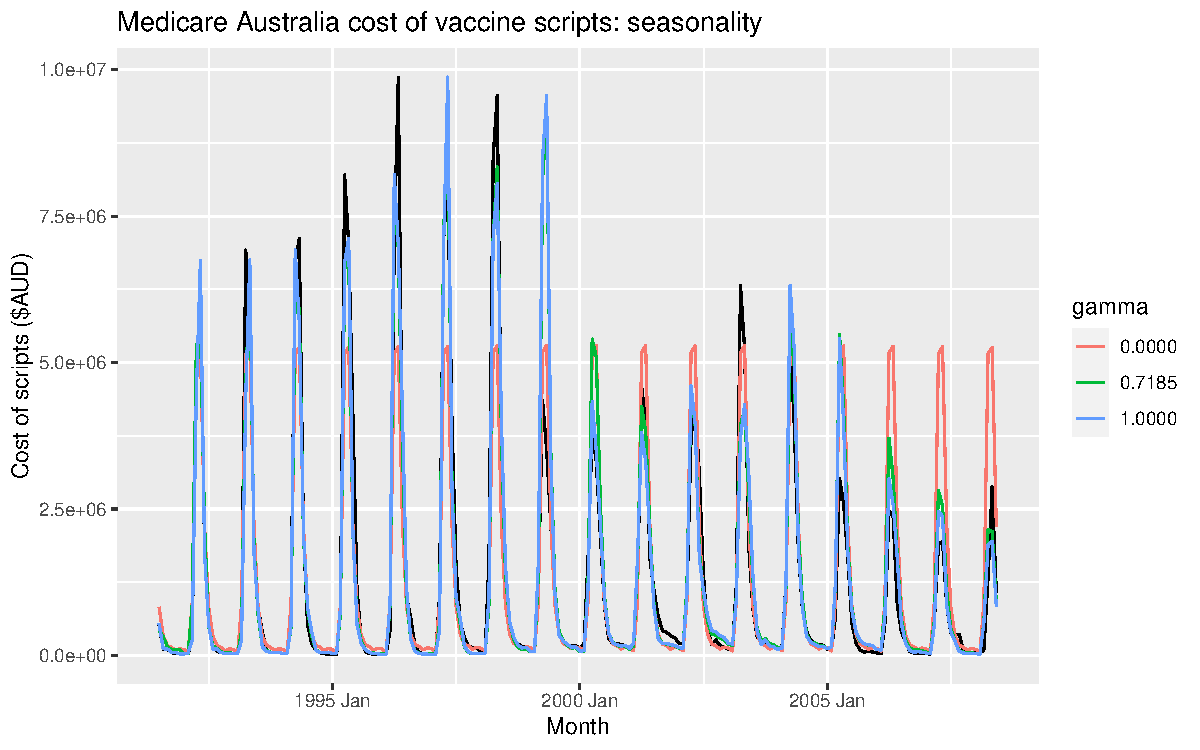
\includegraphics{bookdown-demo_files/figure-latex/gamma-static-1.pdf}

\hypertarget{etsaaa}{%
\subsection{ETS(A,A,A)}\label{etsaaa}}

Holt-Winters additive method with additive errors.

\begin{itemize}
\item
  Forecast equation\} \(\hat{y}_{t+h|t} = \ell_{t} + hb_{t} + s_{t+h-m(k+1)}\)
\item
  Observation equation\} \(y_t=\ell_{t-1}+b_{t-1}+s_{t-m} + \varepsilon_t\)
\item
  State equations\} \[\ell_t=\ell_{t-1}+b_{t-1}+\alpha \varepsilon_t\]
  \[b_t=b_{t-1}+\beta \varepsilon_t\]
  \[s_t = s_{t-m} + \gamma\varepsilon_t\]
\item
  Forecast errors: \(\varepsilon_{t} = y_t - \hat{y}_{t|t-1}\)
\item
  \(k\) is integer part of \((h-1)/m\)
\end{itemize}

\textbf{Activity}

\begin{itemize}
\tightlist
\item
  Write down the model for ETS(A,N,A)
\end{itemize}

\hypertarget{holt-winters-multiplicative-method}{%
\subsection{Holt-Winters multiplicative method}\label{holt-winters-multiplicative-method}}

For when seasonal variations are changing proportional to the level of the series.

\textbf{Component form}

\[\hat{y}{t+h}{t} = (\ell_{t} + hb_{t})s_{t+h-m(k+1)}\]
\[\ell_{t} = \alpha \frac{y_{t}}{s_{t-m}} + (1 - \alpha)(\ell_{t-1} + b_{t-1})\]
b\_\{t\} \&= \[\beta^*(\ell_{t}-\ell_{t-1}) + (1 - \beta^*)b_{t-1}\]
\[s_{t} = \gamma \frac{y_{t}}{(\ell_{t-1} + b_{t-1})} + (1 - \gamma)s_{t-m}\]

\begin{itemize}
\tightlist
\item
  \(k\) is integer part of \((h-1)/m\).
\item
  With additive method \(s_t\) is in absolute terms:\newline within each year \(\sum_i s_i \approx 0\).
\item
  With multiplicative method \(s_t\) is in relative terms:\newline within each year \(\sum_i s_i \approx m\).
\end{itemize}

\hypertarget{etsmam}{%
\subsection{ETS(M,A,M)}\label{etsmam}}

Holt-Winters multiplicative method with multiplicative errors.

\begin{itemize}
\item
  Forecast equation \(\hat{y}_{t+h|t} = (\ell_{t} + hb_{t}) s_{t+h-m(k+1)}\)
\item
  Observation equation \(y_t= (\ell_{t-1}+b_{t-1})s_{t-m}(1 + \varepsilon_t)\)
\item
  State equations \[\ell_t=(\ell_{t-1}+b_{t-1})(1+\alpha \varepsilon_t)\]
  \[b_t=b_{t-1} +\beta(\ell_{t-1}+b_{t-1}) \varepsilon_t\]
  \[s_t = s_{t-m}(1 + \gamma\varepsilon_t)\]
\item
  Forecast errors: \(\varepsilon_{t} = (y_t - \hat{y}_{t|t-1})/\hat{y}_{t|t-1}\)
\item
  \(k\) is integer part of \((h-1)/m\).
\end{itemize}

\hypertarget{example-australian-holiday-tourism}{%
\subsection{Example: Australian holiday tourism}\label{example-australian-holiday-tourism}}

\begin{Shaded}
\begin{Highlighting}[]
\NormalTok{aus_holidays <-}\StringTok{ }\NormalTok{tourism }\OperatorTok
\StringTok{  }\KeywordTok{filter}\NormalTok{(Purpose }\OperatorTok{==}\StringTok{ "Holiday"}\NormalTok{) }\OperatorTok
\StringTok{  }\KeywordTok{summarise}\NormalTok{(}\DataTypeTok{Trips =} \KeywordTok{sum}\NormalTok{(Trips))}
\NormalTok{fit <-}\StringTok{ }\NormalTok{aus_holidays }\OperatorTok
\StringTok{  }\KeywordTok{model}\NormalTok{(}
    \DataTypeTok{additive =} \KeywordTok{ETS}\NormalTok{(Trips }\OperatorTok{~}\StringTok{ }\KeywordTok{error}\NormalTok{(}\StringTok{"A"}\NormalTok{) }\OperatorTok{+}\StringTok{ }\KeywordTok{trend}\NormalTok{(}\StringTok{"A"}\NormalTok{) }\OperatorTok{+}\StringTok{ }\KeywordTok{season}\NormalTok{(}\StringTok{"A"}\NormalTok{)),}
    \DataTypeTok{multiplicative =} \KeywordTok{ETS}\NormalTok{(Trips }\OperatorTok{~}\StringTok{ }\KeywordTok{error}\NormalTok{(}\StringTok{"M"}\NormalTok{) }\OperatorTok{+}\StringTok{ }\KeywordTok{trend}\NormalTok{(}\StringTok{"A"}\NormalTok{) }\OperatorTok{+}\StringTok{ }\KeywordTok{season}\NormalTok{(}\StringTok{"M"}\NormalTok{))}
\NormalTok{  )}
\NormalTok{fc <-}\StringTok{ }\NormalTok{fit }\OperatorTok\StringTok{ }\KeywordTok{forecast}\NormalTok{()}
\end{Highlighting}
\end{Shaded}

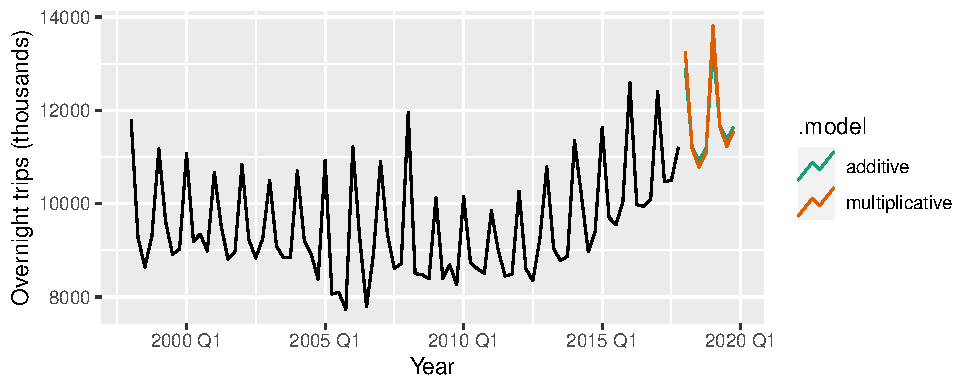
\includegraphics{bookdown-demo_files/figure-latex/unnamed-chunk-35-1.pdf}

\textbf{Estimated components}

\begin{Shaded}
\begin{Highlighting}[]
\KeywordTok{components}\NormalTok{(fit)}
\end{Highlighting}
\end{Shaded}

\begin{verbatim}
## # A dable:                               168 x 7 [1Q]
## # Key:                                   .model [2]
## # ETS(A,A,A) & ETS(M,A,M) Decomposition: Trips = lag(level,
## #   1) + lag(slope, 1) + lag(season, 4) + remainder
##    .model   Quarter  Trips level slope season remainder
##    <chr>      <qtr>  <dbl> <dbl> <dbl>  <dbl>     <dbl>
##  1 additive 1997 Q1    NA    NA   NA    1512.      NA  
##  2 additive 1997 Q2    NA    NA   NA    -290.      NA  
##  3 additive 1997 Q3    NA    NA   NA    -684.      NA  
##  4 additive 1997 Q4    NA  9899. -37.4  -538.      NA  
##  5 additive 1998 Q1 11806. 9964. -24.5  1512.     433. 
##  6 additive 1998 Q2  9276. 9851. -35.6  -290.    -374. 
##  7 additive 1998 Q3  8642. 9700. -50.2  -684.    -489. 
##  8 additive 1998 Q4  9300. 9694. -44.6  -538.     188. 
##  9 additive 1999 Q1 11172. 9652. -44.3  1512.      10.7
## 10 additive 1999 Q2  9608. 9676. -35.6  -290.     290. 
## # ... with 158 more rows
\end{verbatim}

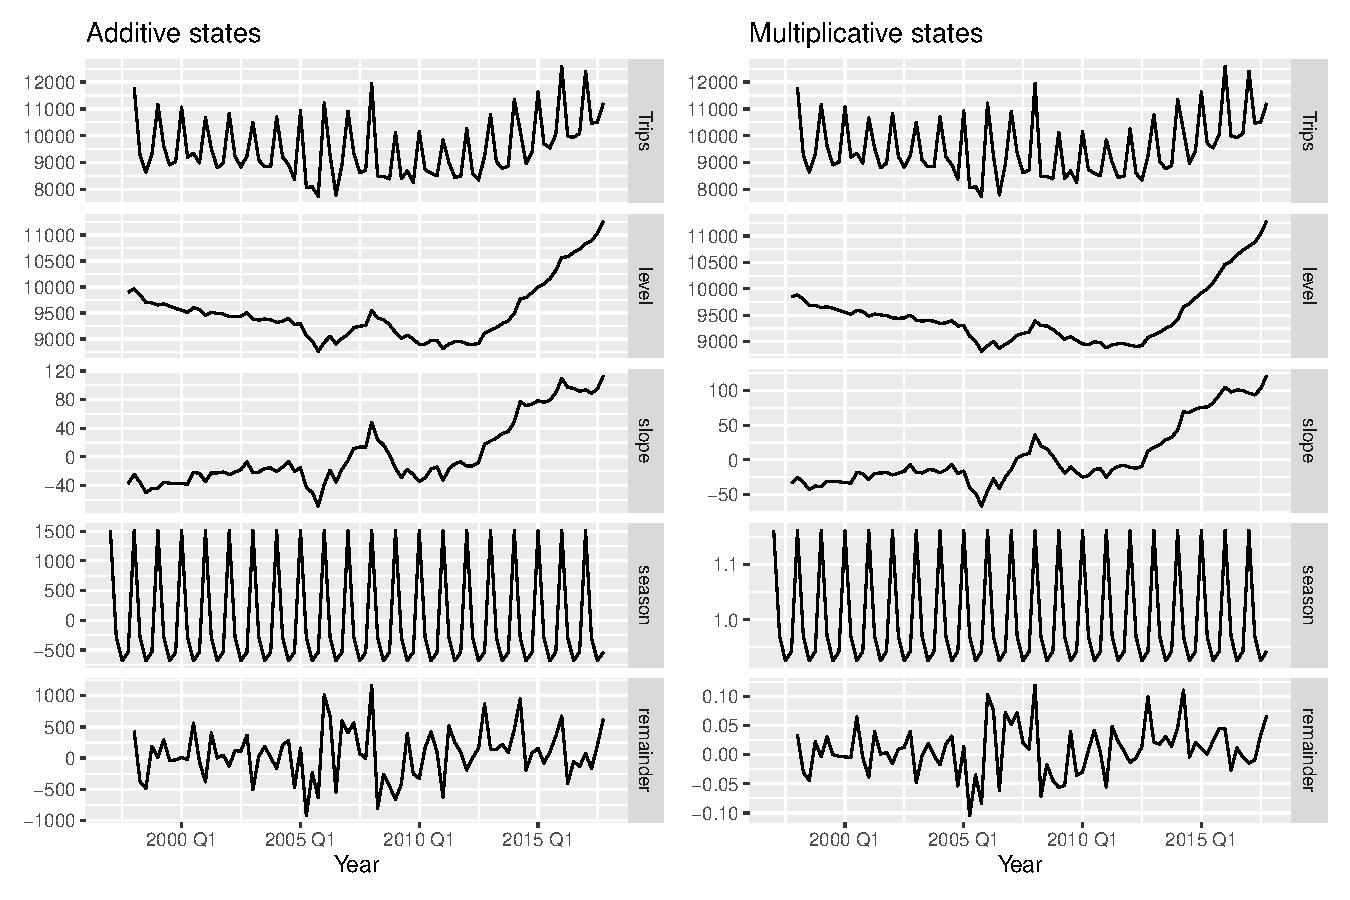
\includegraphics[width=1\linewidth]{bookdown-demo_files/figure-latex/fig-7-LevelTrendSeas-1}

\hypertarget{holt-winters-damped-method}{%
\subsection{Holt-Winters damped method}\label{holt-winters-damped-method}}

Often the single most accurate forecasting method for seasonal data:

\[\hat{y}_{t+h|t} = [\ell_{t} + (\phi+\phi^2 + \dots + \phi^{h})b_{t}]s_{t+h-m(k+1)}\]
\[\ell_{t} = \alpha(y_{t} / s_{t-m}) + (1 - \alpha)(\ell_{t-1} + \phi b_{t-1})\]
\[b_{t} = \beta^*(\ell_{t} - \ell_{t-1}) + (1 - \beta^*)\phi b_{t-1}\]
\[s_{t} = \gamma \frac{y_{t}}{(\ell_{t-1} + \phi b_{t-1})} + (1 - \gamma)s_{t-m}\]

\newpage

\hypertarget{innovations-state-space-models}{%
\section{Innovations state space models}\label{innovations-state-space-models}}

\hypertarget{exponential-smoothing-methods}{%
\subsection{Exponential smoothing methods}\label{exponential-smoothing-methods}}

\begin{table}[H]
\begin{tabular}{lllll}
      &                          & \multicolumn{3}{c}{\textbf{Seasonal Component}} \\
      & \textbf{Trend Component} & N (None)  & A (Additive)  & M (Multiplicative)  \\
N     &    (None)                      &  $(N,N)$          &  $(N,A)$              &       $(N,M)$               \\
A     &     (Additive)                     &  $(A,N)$          &     $(A,A)$          &         $(A,M)$              \\
$A_d$ &  (Additive damped)                         &       $(A_d,N)$    &      $(A_d,A)$          &    $(A_d,M)$                 
\end{tabular}
\end{table}

\begin{itemize}
\tightlist
\item
  \((N,N)\): Simple exponential smoothing
\item
  \((A,N)\): Holt's linear method
\item
  \((A_d,N)\): Additive damped trend method
\item
  \((A,A)\): Additive Holt-Winters' method
\item
  \((A,M)\): Multiplicative Holt-Winters' method
\item
  \((A_d,M)\): Damped multiplicative Holt-Winters' method
\end{itemize}

There are also multiplicative trend methods (not recommended).

\hypertarget{ets-models}{%
\subsection{ETS models}\label{ets-models}}

\textbf{Additive Error}

\begin{table}[h]
\begin{tabular}{lllll}
 &                         & \multicolumn{3}{c}{\textbf{Seasonal Component}} \\
      & \textbf{Trend Component} & N (None)  & A (Additive)  & M (Multiplicative)  \\
N     &    (None)                      &  $(A,N,N)$          &  $(A,N,A)$              &       $(A,N,M)$               \\
A     &     (Additive)                     &  $(A,A,N)$          &     $(A,A,A)$          &         $(A,A,M)$              \\
$A_d$ &  (Additive damped)                         &       $(A,A_d,N)$    &      $(A,A_d,A)$          &    $(A,A_d,M)$                 
\end{tabular}
\end{table}

\textbf{Multiplicative Error}

\begin{table}[h]
\begin{tabular}{lllll}
  &                       & \multicolumn{3}{c}{\textbf{Seasonal Component}} \\
      & \textbf{Trend Component} & N (None)  & A (Additive)  & M (Multiplicative)  \\
N     &    (None)                      &  $(M,N,N)$          &  $(M,N,A)$              &       $(M,N,M)$               \\
A     &     (Additive)                     &  $(M,A,N)$          &     $(M,A,A)$          &         $(M,A,M)$              \\
$A_d$ &  (Additive damped)                         &       $(M,A_d,N)$    &      $(M,A_d,A)$          &    $(M,A_d,M)$                 
\end{tabular}
\end{table}

\hypertarget{additive-error-models}{%
\subsection{Additive error models}\label{additive-error-models}}

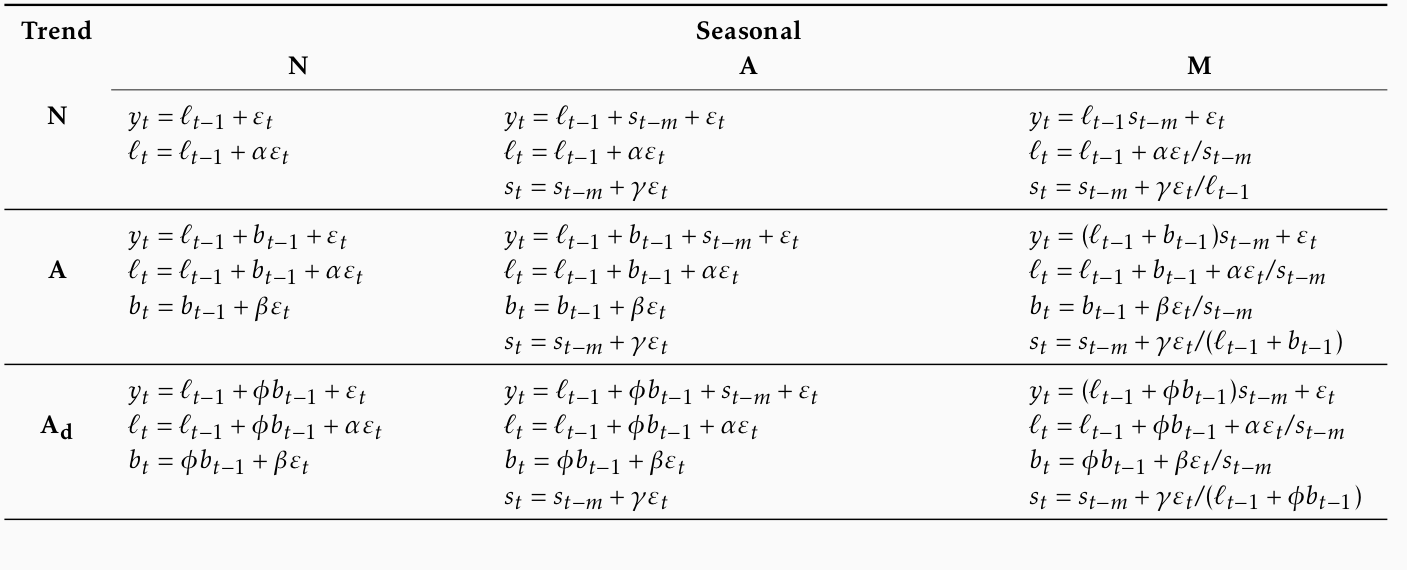
\includegraphics[width=1\textwidth,height=1\textheight]{fig/fig_7_ets_add.png}

\hypertarget{multiplicative-error-models}{%
\subsection{Multiplicative error models}\label{multiplicative-error-models}}

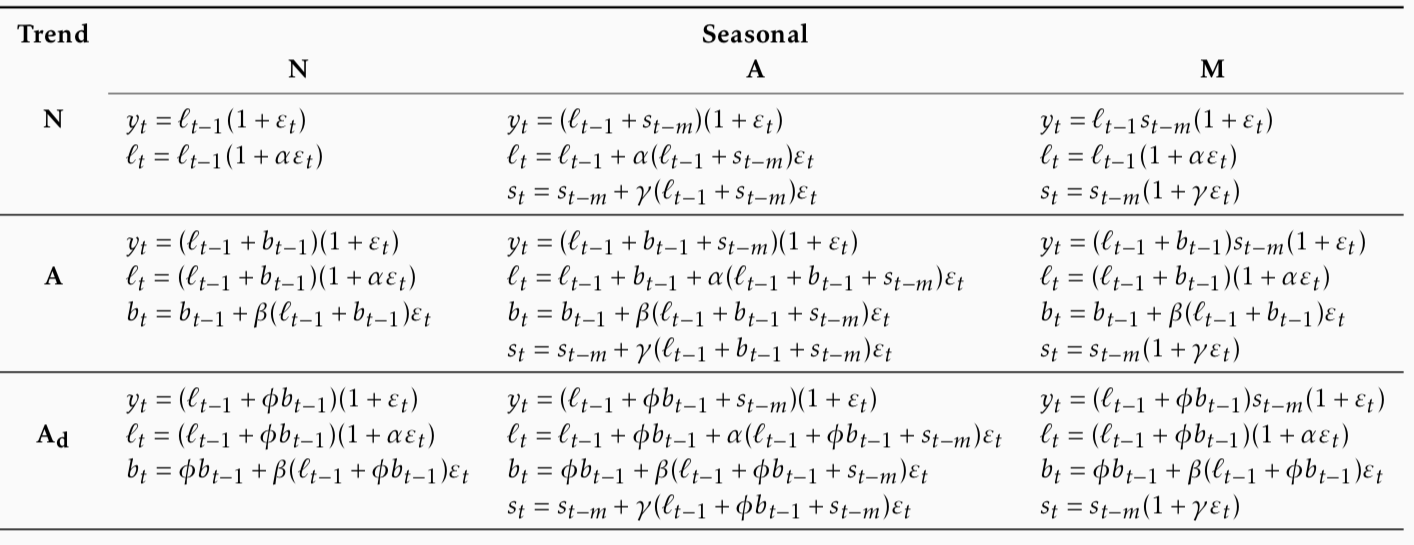
\includegraphics[width=1\textwidth,height=1\textheight]{fig/fig_7_ets_multi.png}

\hypertarget{estimating-ets-models}{%
\subsection{Estimating ETS models}\label{estimating-ets-models}}

\begin{itemize}
\tightlist
\item
  Smoothing parameters \(\alpha\), \(\beta\), \(\gamma\) and \(\phi\), and the initial states \(\ell_0\), \(b_0\), \(s_0,s_{-1},\dots,s_{-m+1}\) are estimated by maximising the ``likelihood'' = the probability of the data arising from the specified model.
\item
  For models with additive errors equivalent to minimising SSE.
\item
  For models with multiplicative errors, \textbf{not} equivalent to minimising SSE.
\end{itemize}

\hypertarget{innovations-state-space-models-1}{%
\subsection{Innovations state space models}\label{innovations-state-space-models-1}}

Let \(\mathbf{x}_t = (\ell_t, b_t, s_t, s_{t-1}, \dots, s_{t-m+1})\) and \(\varepsilon_t\stackrel{\mbox{\scriptsize iid}}{\sim} \mbox{N}(0,\sigma^2)\).

\begin{table}[H]
\begin{tabular}{lcl}
$y_t$ &=& $\underbrace{h(\mathbf{x}_{t-1})} +
\underbrace{k(\mathbf{x}_{t-1})\varepsilon_t}$\\
&& \hspace*{0.5cm}$\mu_t$ \hspace*{1.45cm} $e_t$ \\[0.2cm]
$\mathbf{x}_t$ &=& $f(\mathbf{x}_{t-1}) +
g(\mathbf{x}_{t-1})\varepsilon_t$\\
\end{tabular}
\end{table}

\textbf{Additive errors}

\[k(x)=1. \qquad y_t = \mu_{t} + \varepsilon_t.\]

\textbf{Multiplicative errors}

\[k(\mathbf{x}_{t-1}) = \mu_{t}.\qquad y_t = \mu_{t}(1 + \varepsilon_t).\]
\[\varepsilon_t = (y_t - \mu_t)/\mu_t \text{  is  relative error}.\]

\hypertarget{innovations-state-space-models-2}{%
\subsection{Innovations state space models}\label{innovations-state-space-models-2}}

\textbf{Estimation}

\[L^*(\mathbf\theta,\mathbf{x}_0) = T\log\!\bigg(\sum_{t=1}^T \varepsilon^2_t\!\bigg) + 2\sum_{t=1}^T \log|k(\mathbf{x}_{t-1})|\]
\[= -2\log(\text{Likelihood}) + \mbox{constant}\]

\begin{itemize}
\tightlist
\item
  Estimate parameters \(\mathbf\theta = (\alpha,\beta,\gamma,\phi)\) and
  initial states \(\mathbf{x}_0 = (\ell_0,b_0,s_0,s_{-1},\dots,s_{-m+1})\) by
  minimizing \(L^*\).
\end{itemize}

\hypertarget{parameter-restrictions}{%
\subsection{Parameter restrictions}\label{parameter-restrictions}}

\hypertarget{usual-region}{%
\subsubsection{\texorpdfstring{\emph{Usual} region}{Usual region}}\label{usual-region}}

\begin{itemize}
\tightlist
\item
  Traditional restrictions in the methods \(0< \alpha,\beta^*,\gamma^*,\phi<1\)\newline (equations interpreted as weighted averages).
\item
  In models we set \(\beta=\alpha\beta^*\) and \(\gamma=(1-\alpha)\gamma^*\).
\item
  Therefore \(0< \alpha <1\), ~~ \(0 < \beta < \alpha\) ~~ and \(0< \gamma < 1-\alpha\).
\item
  \(0.8<\phi<0.98\) --- to prevent numerical difficulties.
\end{itemize}

\hypertarget{admissible-region}{%
\subsubsection{\texorpdfstring{\emph{Admissible} region}{Admissible region}}\label{admissible-region}}

\begin{itemize}
\tightlist
\item
  To prevent observations in the distant past having a continuing effect on current forecasts.
\item
  Usually (but not always) less restrictive than the\emph{traditional} region.
\item
  For example for ETS(A,N,N): \newline \textit{traditional} \(0< \alpha <1\) --- \textit{admissible} is \(0< \alpha <2\).
\end{itemize}

\hypertarget{model-selection}{%
\subsection{Model selection}\label{model-selection}}

\textbf{Akaike's Information Criterion}

\[\text{AIC} = -2\log(\text{L}) + 2k\]

where \(L\) is the likelihood and \(k\) is the number of parameters initial states estimated in the model.

\textbf{Corrected AIC}

\[\text{AIC}_{\text{c}} = \text{AIC} + \frac{2(k+1)(k+2)}{T-k}\]
which is the AIC corrected (for small sample bias).

\textbf{Bayesian Information Criterion}

\[\text{BIC} = \text{AIC} + k(\log(T)-2).\]

\hypertarget{aic-and-cross-validation}{%
\subsection{AIC and cross-validation}\label{aic-and-cross-validation}}

Minimizing the AIC assuming Gaussian residuals is asymptotically equivalent to minimizing one-step time series cross validation MSE.

\hypertarget{automatic-forecasting}{%
\subsection{Automatic forecasting}\label{automatic-forecasting}}

\textbf{From Hyndman et al.~(IJF, 2002):}

\begin{itemize}
\tightlist
\item
  Apply each model that is appropriate to the data.
  Optimize parameters and initial values using MLE (or some other
  criterion).
\item
  Select best method using AICc:
\item
  Produce forecasts using best method.
\item
  Obtain forecast intervals using underlying state space model.
\end{itemize}

Method performed very well in M3 competition.

\hypertarget{example-national-populations}{%
\subsection{Example: National populations}\label{example-national-populations}}

\begin{Shaded}
\begin{Highlighting}[]
\NormalTok{fit <-}\StringTok{ }\NormalTok{global_economy }\OperatorTok
\StringTok{  }\KeywordTok{mutate}\NormalTok{(}\DataTypeTok{Pop =}\NormalTok{ Population }\OperatorTok{/}\StringTok{ }\FloatTok{1e6}\NormalTok{) }\OperatorTok
\StringTok{  }\KeywordTok{model}\NormalTok{(}\DataTypeTok{ets =} \KeywordTok{ETS}\NormalTok{(Pop))}
\NormalTok{fit}
\end{Highlighting}
\end{Shaded}

\begin{verbatim}
## # A mable: 263 x 2
## # Key:     Country [263]
##    Country                      ets
##    <fct>                    <model>
##  1 Afghanistan         <ETS(A,A,N)>
##  2 Albania             <ETS(M,A,N)>
##  3 Algeria             <ETS(M,A,N)>
##  4 American Samoa      <ETS(M,A,N)>
##  5 Andorra             <ETS(M,A,N)>
##  6 Angola              <ETS(M,A,N)>
##  7 Antigua and Barbuda <ETS(M,A,N)>
##  8 Arab World          <ETS(M,A,N)>
##  9 Argentina           <ETS(A,A,N)>
## 10 Armenia             <ETS(M,A,N)>
## # ... with 253 more rows
\end{verbatim}

\begin{Shaded}
\begin{Highlighting}[]
\NormalTok{fit }\OperatorTok
\StringTok{  }\KeywordTok{forecast}\NormalTok{(}\DataTypeTok{h =} \DecValTok{5}\NormalTok{)}
\end{Highlighting}
\end{Shaded}

\begin{verbatim}
## # A fable: 1,315 x 5 [1Y]
## # Key:     Country, .model [263]
##    Country     .model  Year             Pop .mean
##    <fct>       <chr>  <dbl>          <dist> <dbl>
##  1 Afghanistan ets     2018    N(36, 0.012) 36.4 
##  2 Afghanistan ets     2019    N(37, 0.059) 37.3 
##  3 Afghanistan ets     2020     N(38, 0.16) 38.2 
##  4 Afghanistan ets     2021     N(39, 0.35) 39.0 
##  5 Afghanistan ets     2022     N(40, 0.64) 39.9 
##  6 Albania     ets     2018 N(2.9, 0.00012)  2.87
##  7 Albania     ets     2019   N(2.9, 6e-04)  2.87
##  8 Albania     ets     2020  N(2.9, 0.0017)  2.87
##  9 Albania     ets     2021  N(2.9, 0.0036)  2.86
## 10 Albania     ets     2022  N(2.9, 0.0066)  2.86
## # ... with 1,305 more rows
\end{verbatim}

\hypertarget{example-australian-holiday-tourism-1}{%
\subsection{Example: Australian holiday tourism}\label{example-australian-holiday-tourism-1}}

\begin{Shaded}
\begin{Highlighting}[]
\NormalTok{holidays <-}\StringTok{ }\NormalTok{tourism }\OperatorTok
\StringTok{  }\KeywordTok{filter}\NormalTok{(Purpose }\OperatorTok{==}\StringTok{ "Holiday"}\NormalTok{)}
\NormalTok{fit <-}\StringTok{ }\NormalTok{holidays }\OperatorTok\StringTok{ }\KeywordTok{model}\NormalTok{(}\DataTypeTok{ets =} \KeywordTok{ETS}\NormalTok{(Trips))}
\NormalTok{fit}
\end{Highlighting}
\end{Shaded}

\begin{verbatim}
## # A mable: 76 x 4
## # Key:     Region, State, Purpose [76]
##    Region                State          Purpose          ets
##    <chr>                 <chr>          <chr>        <model>
##  1 Adelaide              South Austral~ Holiday <ETS(A,N,A)>
##  2 Adelaide Hills        South Austral~ Holiday <ETS(A,A,N)>
##  3 Alice Springs         Northern Terr~ Holiday <ETS(M,N,A)>
##  4 Australia's Coral Co~ Western Austr~ Holiday <ETS(M,N,A)>
##  5 Australia's Golden O~ Western Austr~ Holiday <ETS(M,N,M)>
##  6 Australia's North We~ Western Austr~ Holiday <ETS(A,N,A)>
##  7 Australia's South We~ Western Austr~ Holiday <ETS(M,N,M)>
##  8 Ballarat              Victoria       Holiday <ETS(M,N,A)>
##  9 Barkly                Northern Terr~ Holiday <ETS(A,N,A)>
## 10 Barossa               South Austral~ Holiday <ETS(A,N,N)>
## # ... with 66 more rows
\end{verbatim}

\begin{Shaded}
\begin{Highlighting}[]
\NormalTok{fit }\OperatorTok
\StringTok{  }\KeywordTok{filter}\NormalTok{(Region }\OperatorTok{==}\StringTok{ "Snowy Mountains"}\NormalTok{) }\OperatorTok
\StringTok{  }\KeywordTok{report}\NormalTok{()}
\end{Highlighting}
\end{Shaded}

\begin{verbatim}
## Series: Trips 
## Model: ETS(M,N,A) 
##   Smoothing parameters:
##     alpha = 0.1571 
##     gamma = 0.0001001 
## 
##   Initial states:
##      l     s1    s2     s3     s4
##  141.7 -60.96 130.9 -42.24 -27.66
## 
##   sigma^2:  0.0388
## 
##   AIC  AICc   BIC 
## 852.0 853.6 868.7
\end{verbatim}

\begin{Shaded}
\begin{Highlighting}[]
\NormalTok{fit }\OperatorTok
\StringTok{  }\KeywordTok{filter}\NormalTok{(Region }\OperatorTok{==}\StringTok{ "Snowy Mountains"}\NormalTok{) }\OperatorTok
\StringTok{  }\KeywordTok{components}\NormalTok{(fit)}
\end{Highlighting}
\end{Shaded}

\begin{verbatim}
## # A dable:                  84 x 9 [1Q]
## # Key:                      Region, State, Purpose, .model
## #   [1]
## # ETS(M,N,A) Decomposition: Trips = (lag(level, 1) +
## #   lag(season, 4)) * (1 + remainder)
##    Region State Purpose .model Quarter Trips level season
##    <chr>  <chr> <chr>   <chr>    <qtr> <dbl> <dbl>  <dbl>
##  1 Snowy~ New ~ Holiday ets    1997 Q1  NA     NA   -27.7
##  2 Snowy~ New ~ Holiday ets    1997 Q2  NA     NA   -42.2
##  3 Snowy~ New ~ Holiday ets    1997 Q3  NA     NA   131. 
##  4 Snowy~ New ~ Holiday ets    1997 Q4  NA    142.  -61.0
##  5 Snowy~ New ~ Holiday ets    1998 Q1 101.   140.  -27.7
##  6 Snowy~ New ~ Holiday ets    1998 Q2 112.   142.  -42.2
##  7 Snowy~ New ~ Holiday ets    1998 Q3 310.   148.  131. 
##  8 Snowy~ New ~ Holiday ets    1998 Q4  89.8  148.  -61.0
##  9 Snowy~ New ~ Holiday ets    1999 Q1 112.   147.  -27.7
## 10 Snowy~ New ~ Holiday ets    1999 Q2 103.   147.  -42.2
## # ... with 74 more rows, and 1 more variable:
## #   remainder <dbl>
\end{verbatim}

\begin{Shaded}
\begin{Highlighting}[]
\NormalTok{fit }\OperatorTok
\StringTok{  }\KeywordTok{filter}\NormalTok{(Region }\OperatorTok{==}\StringTok{ "Snowy Mountains"}\NormalTok{) }\OperatorTok
\StringTok{  }\KeywordTok{components}\NormalTok{(fit) }\OperatorTok
\StringTok{  }\KeywordTok{autoplot}\NormalTok{()}
\end{Highlighting}
\end{Shaded}

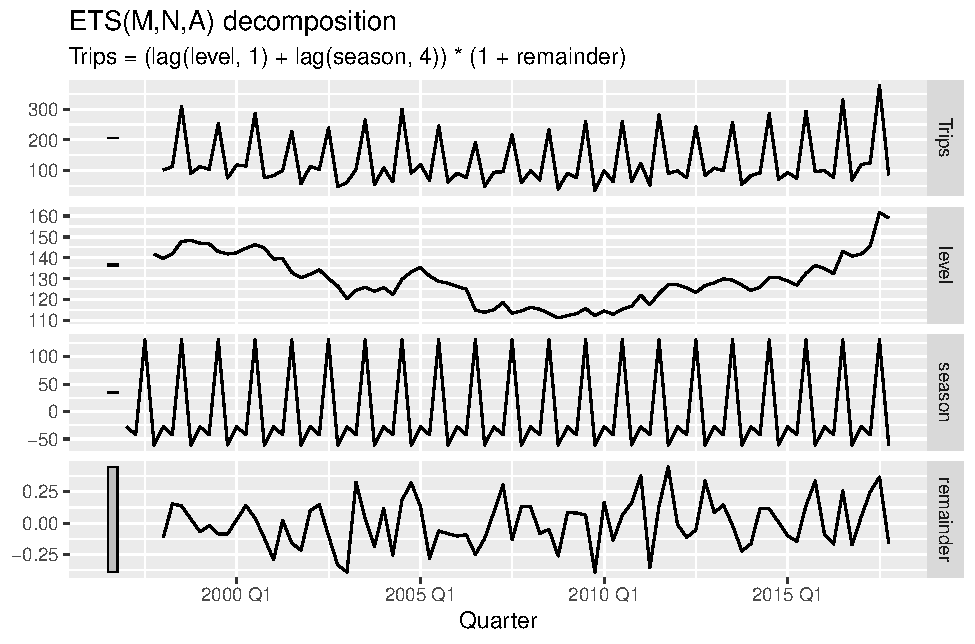
\includegraphics{bookdown-demo_files/figure-latex/ausholidays-components-plot-1.pdf}

\begin{Shaded}
\begin{Highlighting}[]
\NormalTok{fit }\OperatorTok\StringTok{ }\KeywordTok{forecast}\NormalTok{()}
\end{Highlighting}
\end{Shaded}

\begin{verbatim}
## # A fable: 608 x 7 [1Q]
## # Key:     Region, State, Purpose, .model [76]
##    Region   State   Purpose .model Quarter       Trips .mean
##    <chr>    <chr>   <chr>   <chr>    <qtr>      <dist> <dbl>
##  1 Adelaide South ~ Holiday ets    2018 Q1 N(210, 457) 210. 
##  2 Adelaide South ~ Holiday ets    2018 Q2 N(173, 473) 173. 
##  3 Adelaide South ~ Holiday ets    2018 Q3 N(169, 489) 169. 
##  4 Adelaide South ~ Holiday ets    2018 Q4 N(186, 505) 186. 
##  5 Adelaide South ~ Holiday ets    2019 Q1 N(210, 521) 210. 
##  6 Adelaide South ~ Holiday ets    2019 Q2 N(173, 537) 173. 
##  7 Adelaide South ~ Holiday ets    2019 Q3 N(169, 553) 169. 
##  8 Adelaide South ~ Holiday ets    2019 Q4 N(186, 569) 186. 
##  9 Adelaid~ South ~ Holiday ets    2018 Q1   N(19, 36)  19.4
## 10 Adelaid~ South ~ Holiday ets    2018 Q2   N(20, 36)  19.6
## # ... with 598 more rows
\end{verbatim}

\begin{Shaded}
\begin{Highlighting}[]
\NormalTok{fit }\OperatorTok
\StringTok{  }\KeywordTok{forecast}\NormalTok{() }\OperatorTok
\StringTok{  }\KeywordTok{filter}\NormalTok{(Region }\OperatorTok{==}\StringTok{ "Snowy Mountains"}\NormalTok{) }\OperatorTok
\StringTok{  }\KeywordTok{autoplot}\NormalTok{(holidays) }\OperatorTok{+}
\StringTok{  }\KeywordTok{xlab}\NormalTok{(}\StringTok{"Year"}\NormalTok{) }\OperatorTok{+}\StringTok{ }\KeywordTok{ylab}\NormalTok{(}\StringTok{"Overnight trips (thousands)"}\NormalTok{)}
\end{Highlighting}
\end{Shaded}

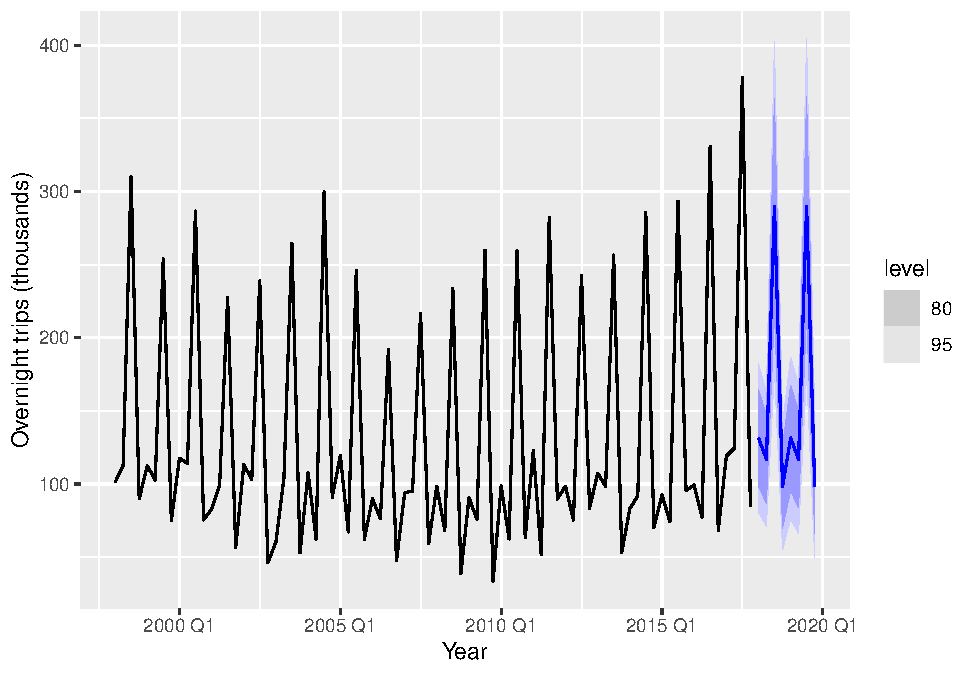
\includegraphics{bookdown-demo_files/figure-latex/ausholidays-forecast-plot-1.pdf}

\hypertarget{some-unstable-models}{%
\subsection{Some unstable models}\label{some-unstable-models}}

\begin{itemize}
\tightlist
\item
  Some of the combinations of (Error, Trend, Seasonal) can lead to numerical difficulties; see equations with division by a state.
\item
  These are: ETS(A,N,M), ETS(A,A,M), ETS(A,\(A_d\),M).
\item
  Models with multiplicative errors are useful for strictly positive data, but are not numerically stable with data containing zeros or negative values. In that case only the six fully additive models will be applied.
\end{itemize}

\hypertarget{exponential-smoothing-models}{%
\subsection{Exponential smoothing models}\label{exponential-smoothing-models}}

\textbf{Additive Error}

\begin{table}[H]
\begin{tabular}{lllll}
 &                         & \multicolumn{3}{c}{\textbf{Seasonal Component}} \\
      & \textbf{Trend Component} & N (None)  & A (Additive)  & M (Multiplicative)  \\
N     &    (None)                      &  $(A,N,N)$          &  $(A,N,A)$              &                 \\
A     &     (Additive)                     &  $(A,A,N)$          &     $(A,A,A)$          &                  \\
$A_d$ &  (Additive damped)                         &       $(A,A_d,N)$    &      $(A,A_d,A)$          &                 
\end{tabular}
\end{table}

\newpage

\textbf{Multiplicative Error}

\begin{table}[H]
\begin{tabular}{lllll}
  &                       & \multicolumn{3}{c}{\textbf{Seasonal Component}} \\
      & \textbf{Trend Component} & N (None)  & A (Additive)  & M (Multiplicative)  \\
N     &    (None)                      &  $(M,N,N)$          &  $(M,N,A)$              &       $(M,N,M)$               \\
A     &     (Additive)                     &  $(M,A,N)$          &     $(M,A,A)$          &         $(M,A,M)$              \\
$A_d$ &  (Additive damped)                         &       $(M,A_d,N)$    &      $(M,A_d,A)$          &    $(M,A_d,M)$                 
\end{tabular}
\end{table}

\hypertarget{residuals}{%
\subsection{Residuals}\label{residuals}}

\textbf{Response residuals}

\[\hat{e}_t = y_t - \hat{y}_{t|t-1}\]

\textbf{Innovation residuals}

Additive error model:
\[\hat\varepsilon_t = y_t - \hat{y}_{t|t-1}\]

Multiplicative error model:
\[\hat\varepsilon_t = \frac{y_t - \hat{y}_{t|t-1}}{\hat{y}_{t|t-1}}\]

\hypertarget{example-australian-holiday-tourism-2}{%
\subsection{Example: Australian holiday tourism}\label{example-australian-holiday-tourism-2}}

\begin{Shaded}
\begin{Highlighting}[]
\NormalTok{aus_holidays <-}\StringTok{ }\NormalTok{tourism }\OperatorTok
\StringTok{  }\KeywordTok{filter}\NormalTok{(Purpose }\OperatorTok{==}\StringTok{ "Holiday"}\NormalTok{) }\OperatorTok
\StringTok{  }\KeywordTok{summarise}\NormalTok{(}\DataTypeTok{Trips =} \KeywordTok{sum}\NormalTok{(Trips))}
\NormalTok{fit <-}\StringTok{ }\NormalTok{aus_holidays }\OperatorTok
\StringTok{  }\KeywordTok{model}\NormalTok{(}\DataTypeTok{ets =} \KeywordTok{ETS}\NormalTok{(Trips)) }\OperatorTok
\StringTok{  }\KeywordTok{report}\NormalTok{()}
\end{Highlighting}
\end{Shaded}

\begin{verbatim}
## Series: Trips 
## Model: ETS(M,N,M) 
##   Smoothing parameters:
##     alpha = 0.3578 
##     gamma = 0.0009686 
## 
##   Initial states:
##     l    s1     s2     s3    s4
##  9667 0.943 0.9268 0.9684 1.162
## 
##   sigma^2:  0.0022
## 
##  AIC AICc  BIC 
## 1331 1333 1348
\end{verbatim}

\begin{Shaded}
\begin{Highlighting}[]
\KeywordTok{residuals}\NormalTok{(fit)}
\KeywordTok{residuals}\NormalTok{(fit, }\DataTypeTok{type =} \StringTok{"response"}\NormalTok{)}
\end{Highlighting}
\end{Shaded}

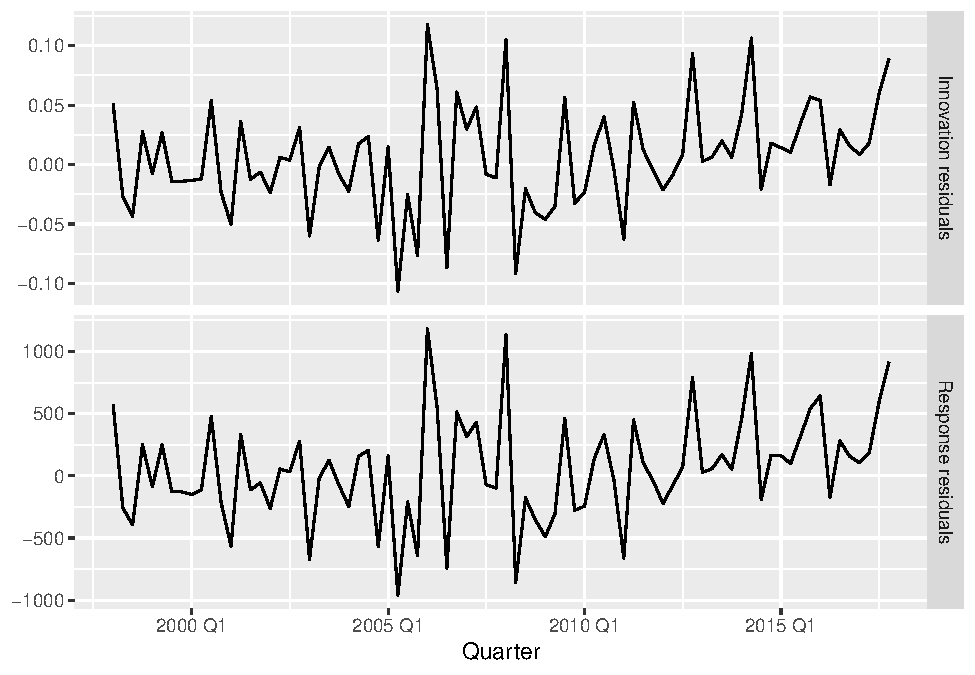
\includegraphics{bookdown-demo_files/figure-latex/unnamed-chunk-39-1.pdf}

\hypertarget{forecasting-with-exponential-smoothing}{%
\section{Forecasting with exponential smoothing}\label{forecasting-with-exponential-smoothing}}

\hypertarget{forecasting-with-ets-models}{%
\subsection{Forecasting with ETS models}\label{forecasting-with-ets-models}}

\textbf{Point forecasts:} iterate the equations for \(t=T+1,T+2,\dots,T+h\) and set all \(\varepsilon_t=0\) for \(t>T\).

\begin{itemize}
\tightlist
\item
  Not the same as \(\text{E}(y_{t+h} | \mathbf{x}_t)\) unless trend and seasonality are both additive.
\item
  Point forecasts for ETS(A,\emph{,}) are identical to ETS(M,\emph{,}) if the parameters are the same.
\end{itemize}

\hypertarget{example-etsaan}{%
\subsection{Example: ETS(A,A,N)}\label{example-etsaan}}

\[y_{T+1} = \ell_T + b_T  + \varepsilon_{T+1}\]
\[\hat{y}_{T+1|T} = \ell_{T}+b_{T}\]
\[y_{T+2}       = \ell_{T+1} + b_{T+1} + \varepsilon_{T+2}\]
\[=
                      (\ell_T + b_T + \alpha\varepsilon_{T+1}) +
                      (b_T + \beta \varepsilon_{T+1}) +
        \varepsilon_{T+2}\]
\[\hat{y}_{T+2|T} = \ell_{T}+2b_{T}\]
etc.

\hypertarget{example-etsman}{%
\subsection{Example: ETS(M,A,N)}\label{example-etsman}}

\[y_{T+1} = (\ell_T + b_T )(1+ \varepsilon_{T+1})\]
\[\hat{y}_{T+1|T} = \ell_{T}+b_{T}.\]
\[y_{T+2}         = (\ell_{T+1} + b_{T+1})(1 + \varepsilon_{T+2})\]
\[= \left\{
                    (\ell_T + b_T) (1+ \alpha\varepsilon_{T+1}) +
                    \left[b_T + \beta (\ell_T + b_T)\varepsilon_{T+1}\right]
                    \right\}
                   (1 + \varepsilon_{T+2})\]
\[\hat{y}_{T+2|T} = \ell_{T}+2b_{T}\]
etc.

\hypertarget{forecasting-with-ets-models-1}{%
\subsection{Forecasting with ETS models}\label{forecasting-with-ets-models-1}}

\textbf{Prediction intervals:} can only generated using the models.

\begin{itemize}
\tightlist
\item
  The prediction intervals will differ between models with additive and multiplicative errors.
\item
  Exact formulae for some models.
\item
  More general to simulate future sample paths, conditional on the last estimate of the states, and to obtain prediction intervals from the percentiles of these simulated future paths.
\end{itemize}

\hypertarget{prediction-intervals-1}{%
\subsection{Prediction intervals}\label{prediction-intervals-1}}

PI for most ETS models: \(\hat{y}_{T+h|T} \pm c \sigma_h\), where \(c\) depends on coverage probability and \(\sigma_h\) is forecast standard deviation.

\begin{tabular}{ll}
\hline
(A,N,N) & $\sigma_h = \sigma^2\big[1 + \alpha^2(h-1)\big]$\\
(A,A,N) & $\sigma_h = \sigma^2\Big[1 + (h-1)\big\{\alpha^2 + \alpha\beta h + \frac16\beta^2h(2h-1)\big\}\Big]$\\
(A,A$_d$,N) & $\sigma_h = \sigma^2\biggl[1 + \alpha^2(h-1) + \frac{\beta\phi h}{(1-\phi)^2} \left\{2\alpha(1-\phi) +\beta\phi\right\}$\\
      & \hspace*{1.5cm}$\mbox{} - \frac{\beta\phi(1-\phi^h)}{(1-\phi)^2(1-\phi^2)} \left\{ 2\alpha(1-\phi^2)+ \beta\phi(1+2\phi-\phi^h)\right\}\biggr]$\\
(A,N,A) &              $\sigma_h = \sigma^2\Big[1 + \alpha^2(h-1) + \gamma k(2\alpha+\gamma)\Big]$\\
(A,A,A) &              $\sigma_h = \sigma^2\Big[1 + (h-1)\big\{\alpha^2 + \alpha\beta h + \frac16\beta^2h(2h-1)\big\} + \gamma k \big\{2\alpha+ \gamma + \beta m (k+1)\big\} \Big]$\\
(A,A$_d$,A) &  $\sigma_h = \sigma^2\biggl[1 + \alpha^2(h-1) +\frac{\beta\phi h}{(1-\phi)^2} \left\{2\alpha(1-\phi)  + \beta\phi \right\}$\\
  & \hspace*{1.5cm}$\mbox{} - \frac{\beta\phi(1-\phi^h)}{(1-\phi)^2(1-\phi^2)} \left\{ 2\alpha(1-\phi^2)+ \beta\phi(1+2\phi-\phi^h)\right\}$ \\
  & \hspace*{1.5cm}$\mbox{} + \gamma k(2\alpha+\gamma)  + \frac{2\beta\gamma\phi}{(1-\phi)(1-\phi^m)}\left\{k(1-\phi^m) - \phi^m(1-\phi^{mk})\right\}\biggr]$
\end{tabular}

\newpage

\hypertarget{example-corticosteroid-drug-sales}{%
\subsection{Example: Corticosteroid drug sales}\label{example-corticosteroid-drug-sales}}

\begin{Shaded}
\begin{Highlighting}[]
\NormalTok{h02 <-}\StringTok{ }\NormalTok{PBS }\OperatorTok
\StringTok{  }\KeywordTok{filter}\NormalTok{(ATC2 }\OperatorTok{==}\StringTok{ "H02"}\NormalTok{) }\OperatorTok
\StringTok{  }\KeywordTok{summarise}\NormalTok{(}\DataTypeTok{Cost =} \KeywordTok{sum}\NormalTok{(Cost))}
\NormalTok{h02 }\OperatorTok
\StringTok{  }\KeywordTok{autoplot}\NormalTok{(Cost)}
\end{Highlighting}
\end{Shaded}

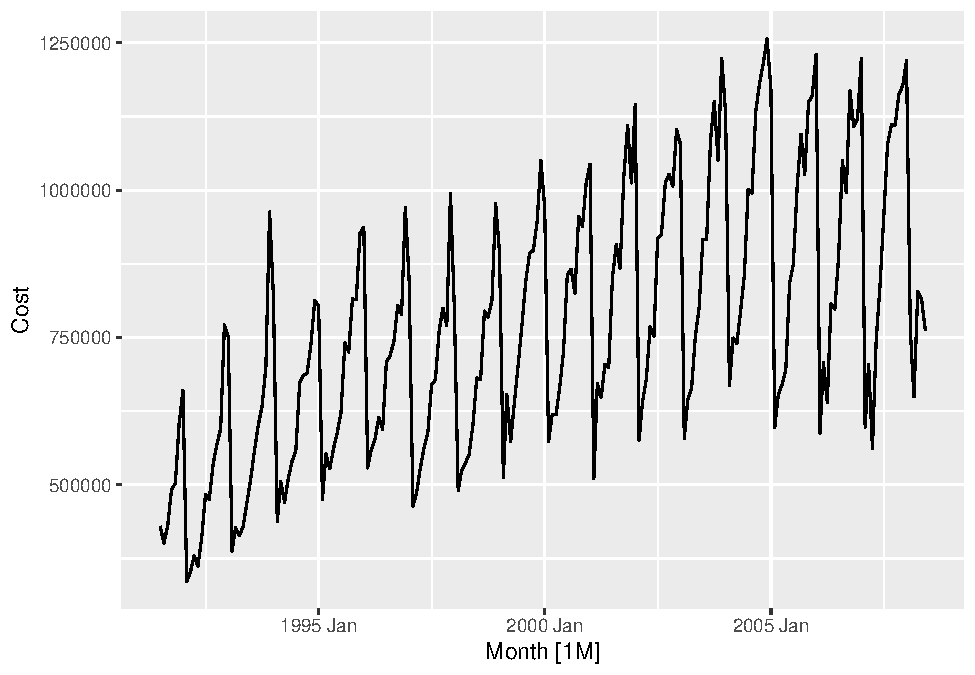
\includegraphics{bookdown-demo_files/figure-latex/h02-plot-1.pdf}

\begin{Shaded}
\begin{Highlighting}[]
\NormalTok{h02 }\OperatorTok
\StringTok{  }\KeywordTok{model}\NormalTok{(}\KeywordTok{ETS}\NormalTok{(Cost)) }\OperatorTok
\StringTok{  }\KeywordTok{report}\NormalTok{()}
\end{Highlighting}
\end{Shaded}

\begin{verbatim}
## Series: Cost 
## Model: ETS(M,Ad,M) 
##   Smoothing parameters:
##     alpha = 0.3071 
##     beta  = 0.0001007 
##     gamma = 0.0001007 
##     phi   = 0.9775 
## 
##   Initial states:
##       l    b     s1    s2     s3     s4     s5    s6    s7
##  417269 8206 0.8717 0.826 0.7563 0.7733 0.6872 1.284 1.325
##    s8    s9   s10   s11    s12
##  1.18 1.164 1.105 1.048 0.9806
## 
##   sigma^2:  0.0046
## 
##  AIC AICc  BIC 
## 5515 5519 5575
\end{verbatim}

\begin{Shaded}
\begin{Highlighting}[]
\NormalTok{h02 }\OperatorTok
\StringTok{  }\KeywordTok{model}\NormalTok{(}\KeywordTok{ETS}\NormalTok{(Cost }\OperatorTok{~}\StringTok{ }\KeywordTok{error}\NormalTok{(}\StringTok{"A"}\NormalTok{) }\OperatorTok{+}\StringTok{ }\KeywordTok{trend}\NormalTok{(}\StringTok{"A"}\NormalTok{) }\OperatorTok{+}\StringTok{ }\KeywordTok{season}\NormalTok{(}\StringTok{"A"}\NormalTok{))) }\OperatorTok
\StringTok{  }\KeywordTok{report}\NormalTok{()}
\end{Highlighting}
\end{Shaded}

\begin{verbatim}
## Series: Cost 
## Model: ETS(A,A,A) 
##   Smoothing parameters:
##     alpha = 0.1702 
##     beta  = 0.006311 
##     gamma = 0.4546 
## 
##   Initial states:
##       l    b     s1      s2      s3      s4      s5     s6
##  409706 9097 -99075 -136602 -191496 -174531 -241437 210644
##      s7     s8     s9   s10   s11    s12
##  244644 145368 130570 84458 39132 -11674
## 
##   sigma^2:  3.499e+09
## 
##  AIC AICc  BIC 
## 5585 5589 5642
\end{verbatim}

\begin{Shaded}
\begin{Highlighting}[]
\NormalTok{h02 }\OperatorTok\StringTok{ }\KeywordTok{model}\NormalTok{(}\KeywordTok{ETS}\NormalTok{(Cost)) }\OperatorTok\StringTok{ }\KeywordTok{forecast}\NormalTok{() }\OperatorTok\StringTok{ }\KeywordTok{autoplot}\NormalTok{(h02)}
\end{Highlighting}
\end{Shaded}

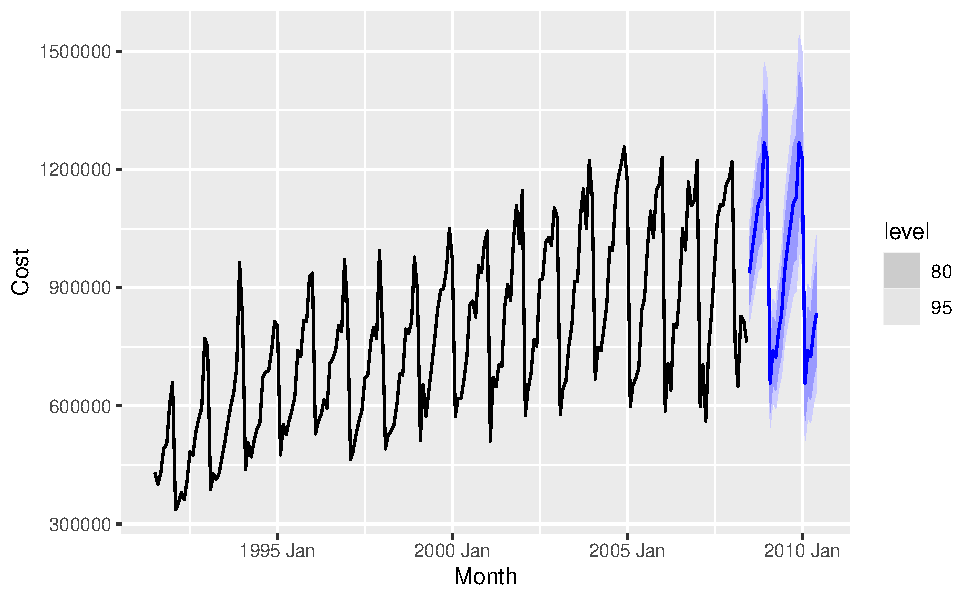
\includegraphics{bookdown-demo_files/figure-latex/unnamed-chunk-42-1.pdf}

\begin{Shaded}
\begin{Highlighting}[]
\NormalTok{h02 }\OperatorTok
\StringTok{  }\KeywordTok{model}\NormalTok{(}
    \DataTypeTok{auto =} \KeywordTok{ETS}\NormalTok{(Cost),}
    \DataTypeTok{AAA =} \KeywordTok{ETS}\NormalTok{(Cost }\OperatorTok{~}\StringTok{ }\KeywordTok{error}\NormalTok{(}\StringTok{"A"}\NormalTok{) }\OperatorTok{+}\StringTok{ }\KeywordTok{trend}\NormalTok{(}\StringTok{"A"}\NormalTok{) }\OperatorTok{+}\StringTok{ }\KeywordTok{season}\NormalTok{(}\StringTok{"A"}\NormalTok{))}
\NormalTok{  ) }\OperatorTok
\StringTok{  }\KeywordTok{accuracy}\NormalTok{()}
\end{Highlighting}
\end{Shaded}

\begin{tabular}{lrrrrr}
\toprule
Model & ME & MAE & RMSE & MAPE & MASE\\
\midrule
auto & 2461 & 38649 & 51102 & 4.989 & 0.6376\\
AAA & -5780 & 43378 & 56784 & 6.048 & 0.7156\\
\bottomrule
\end{tabular}

\hypertarget{arima-vs-ets}{%
\section{ARIMA vs ETS}\label{arima-vs-ets}}

\begin{itemize}
\item
  Myth that ARIMA models are more general than exponential smoothing.
\item
  Linear exponential smoothing models all special cases of ARIMA models.
\item
  Non-linear exponential smoothing models have no equivalent ARIMA counterparts.
\item
  Many ARIMA models have no exponential smoothing counterparts.
\item
  ETS models all non-stationary. Models with seasonality or non-damped trend (or both) have two unit roots; all other models have one unit \rlap{root.}
\end{itemize}

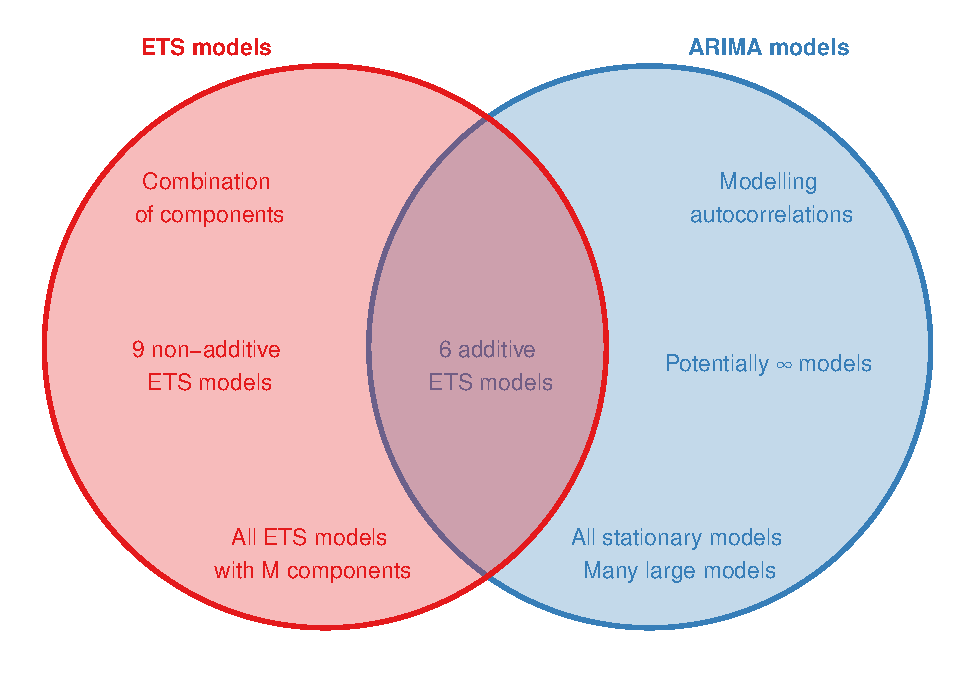
\includegraphics{bookdown-demo_files/figure-latex/venn-1.pdf}

\newpage

\hypertarget{equivalences}{%
\subsection{Equivalences}\label{equivalences}}

\begin{longtable}[]{@{}lll@{}}
\toprule
\textbf{ETS model} & \textbf{ARIMA model} & \textbf{Parameters}\tabularnewline
\midrule
\endhead
ETS(A,N,N) & ARIMA(0,1,1) & \(\theta_1 = \alpha-1\)\tabularnewline
ETS(A,A,N) & ARIMA(0,2,2) & \(\theta_1 = \alpha+\beta-2\)\tabularnewline
& & \(\theta_2 = 1-\alpha\)\tabularnewline
ETS(A,\(A_d\),N) & ARIMA(1,1,2) & \(\phi_1=\phi\)\tabularnewline
& & \(\theta_1 = \alpha+\phi\beta-1-\phi\)\tabularnewline
& & \(\theta_2 = (1-\alpha)\phi\)\tabularnewline
ETS(A,N,A) & ARIMA(0,0,\(m\))(0,1,0)\(_m\) &\tabularnewline
ETS(A,A,A) & ARIMA(0,1,\(m+1\))(0,1,0)\(_m\) &\tabularnewline
ETS(A,\(A_d\),A) & ARIMA(1,0,\(m+1\))(0,1,0)\(_m\) &\tabularnewline
\bottomrule
\end{longtable}

\hypertarget{references-1}{%
\section{References:}\label{references-1}}

\begin{itemize}
\tightlist
\item
  Hyndman, R. J., \& Athanasopoulos, G. (2018). Forecasting: principles and practice. OTexts.
\end{itemize}

\newpage

\hypertarget{volatility-models}{%
\chapter{Volatility Models}\label{volatility-models}}

\pagenumbering{arabic}

\hypertarget{introduction-1}{%
\section{Introduction}\label{introduction-1}}

\begin{itemize}
\tightlist
\item
  Anything that is observed sequentially over time is a time series.
\end{itemize}

\begin{itemize}
\tightlist
\item
  \textbf{Financial time series} analysis focuses on the theory and practice of asset valuation over time.
\end{itemize}

\begin{itemize}
\tightlist
\item
  In finance, the data can be collected much more frequently -- High frequency data.
\end{itemize}

\begin{itemize}
\tightlist
\item
  Many financial time series also exhibit changing variance and this can have important consequences
  in formulating financial decisions.
\end{itemize}

\textbf{Example: Financial time series}

\begin{itemize}
\tightlist
\item
  Typically, when we analyze assets, we look at the percentage change in prices or returns.
\end{itemize}

\begin{Shaded}
\begin{Highlighting}[]
\CommentTok{# Tidy financial analysis }
\KeywordTok{library}\NormalTok{(tidyquant)}

\NormalTok{sp500 <-}\StringTok{ }\KeywordTok{tq_get}\NormalTok{(}\StringTok{"^GSPC"}\NormalTok{, }\DataTypeTok{from =} \StringTok{"1995-01-04"}\NormalTok{, }\DataTypeTok{to =} \StringTok{"2021-02-25"}\NormalTok{ )}
\KeywordTok{print}\NormalTok{(sp500)}
\end{Highlighting}
\end{Shaded}

\begin{verbatim}
## # A tibble: 6,582 x 8
##    symbol date        open  high   low close volume adjusted
##    <chr>  <date>     <dbl> <dbl> <dbl> <dbl>  <dbl>    <dbl>
##  1 ^GSPC  1995-01-04  459.  461.  458.  461. 3.20e8     461.
##  2 ^GSPC  1995-01-05  461.  461.  460.  460. 3.09e8     460.
##  3 ^GSPC  1995-01-06  460.  462.  459.  461. 3.08e8     461.
##  4 ^GSPC  1995-01-09  461.  462.  460.  461. 2.79e8     461.
##  5 ^GSPC  1995-01-10  461.  465.  461.  462. 3.52e8     462.
##  6 ^GSPC  1995-01-11  462.  464.  459.  462. 3.46e8     462.
##  7 ^GSPC  1995-01-12  462.  462.  461.  462. 3.13e8     462.
##  8 ^GSPC  1995-01-13  462.  466.  462.  466. 3.37e8     466.
##  9 ^GSPC  1995-01-16  466.  470.  466.  469. 3.16e8     469.
## 10 ^GSPC  1995-01-17  469.  470.  468.  470. 3.32e8     470.
## # ... with 6,572 more rows
\end{verbatim}

\begin{Shaded}
\begin{Highlighting}[]
\CommentTok{# Convert each assets raw adjusted closing prices to returns}
\NormalTok{sp500_return <-}\StringTok{ }\NormalTok{sp500 }\OperatorTok\StringTok{ }
\StringTok{  }\KeywordTok{tq_transmute}\NormalTok{(}\DataTypeTok{select     =}\NormalTok{ adjusted, }
               \DataTypeTok{mutate_fun =}\NormalTok{ periodReturn, }
               \DataTypeTok{period     =} \StringTok{"daily"}\NormalTok{)}

\NormalTok{sp500_return }\OperatorTok\StringTok{ }
\StringTok{  }\KeywordTok{as_tsibble}\NormalTok{(}\DataTypeTok{index =}\NormalTok{ date) }\OperatorTok
\StringTok{  }\KeywordTok{autoplot}\NormalTok{(daily.returns) }\OperatorTok{+}
\StringTok{  }\KeywordTok{labs}\NormalTok{(}\DataTypeTok{x =} \StringTok{"Day"}\NormalTok{, }\DataTypeTok{y=} \StringTok{"Daily return"}\NormalTok{)}
\end{Highlighting}
\end{Shaded}

\begin{figure}
\centering
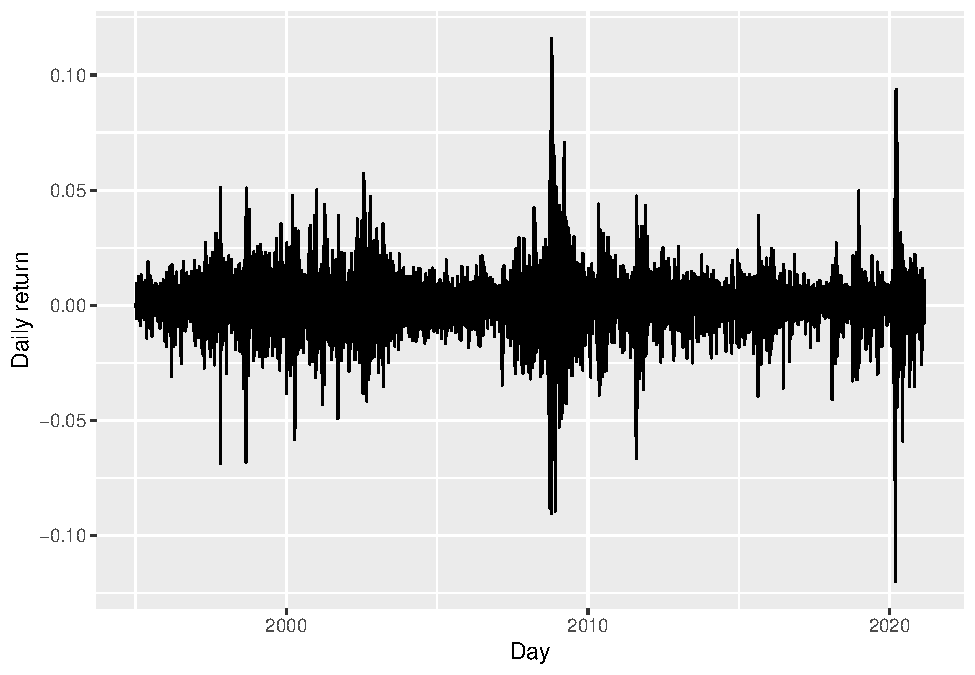
\includegraphics{bookdown-demo_files/figure-latex/sp500-1.pdf}
\caption{\label{fig:sp500}Daily returns of the adjusted closing prices of the S\&P500 index from January 4, 1995 to February 25, 2021}
\end{figure}

\hypertarget{references-2}{%
\section{References:}\label{references-2}}

\begin{itemize}
\tightlist
\item
  Chatfield, C., \& Xing, H. (2019). The analysis of time series: an introduction with R. CRC press.
\end{itemize}

\newpage

\hypertarget{multivariate-time-series-modeliing}{%
\chapter{Multivariate Time Series Modeliing}\label{multivariate-time-series-modeliing}}

\pagenumbering{arabic}

\hypertarget{references-3}{%
\section{References:}\label{references-3}}

\begin{itemize}
\tightlist
\item
  Chatfield, C., \& Xing, H. (2019). The analysis of time series: an introduction with R. CRC press.
\end{itemize}

\bibliography{book.bib,packages.bib}

\end{document}
